\documentclass[lang=en,12pt,newtx]{elegantbook}

\title{XJTLU PGRS Unofficial Guide}
% \subtitle{~~~~~~~~~~~~~~~~~~~~~~~~~~~~~~~~~~~~version v1.1.0}

\author{\KW, \SZ}
% \institute{}
\date{\today}
\version{v1.1.0}
\bioinfo{Repository}{\href{https://github.com/xp-pgrs-unofficial-guide/xp_pgrs_unofficial_guide/releases}{GitHub (latest)} or \space \href{https://xjtlums.sharepoint.com/:u:/s/PGRSUnofficialGuide/ESNKWXoSeJtOpLoqpQXH0UsBWhQnD2SQoFVJx11oR9fV6A?e=x1dAOA}{SharePoint (backup, XJTLU account required)}}

% \bioinfo{customize}{info}

\extrainfo{Standing on the shoulders of giants} 

\setcounter{tocdepth}{3}

% \logo{logo-blue.png} 
\cover{cover3.jpg}

% commands
\usepackage{array}
\usepackage{float}
\usepackage{ulem}
\usepackage{xurl}
\usepackage[export]{adjustbox}
\usepackage{subcaption}
\usepackage{xcolor}
\usepackage{tcolorbox}

\newcommand{\ccr}[1]{\makecell{{\color{#1}\rule{1cm}{1cm}}}}
\newcommand{\emptyline}{\vspace{5mm}}
\newenvironment{newminipage}[1][0.55]
    {   \setlength{\parindent}{0\ccwd}
        \begin{minipage}{#1\textwidth}
            \setlength{\parindent}{2\ccwd}
    }
    {   \end{minipage}
        \setlength{\parindent}{2\ccwd}
    }

% define color in the cover page
\definecolor{customcolor}{RGB}{3,31,115}
\colorlet{coverlinecolor}{customcolor}
\usepackage{cprotect}

\begin{document}

\maketitle
\frontmatter

% Below preface needs to be modified into English
\chapter{Preface}
\thispagestyle{empty}
When I previously communicated with some PhD students, some of them were about to graduate, yet they didn't know they could get office supplies, and some didn't even know where the school gym was, let alone the free fitness room and court resources. Additionally, in the PhD student WeChat group, every year there are people who only find out about the meeting record requirement when it's time for their first APR. Furthermore, even fewer people know about the vast digital resources available under the Liverpool account. Some important things are unknown to oneself, the supervisor, and the office mates, and it might only be discovered upon graduation.

This is the purpose of initiating this guide project. Although every student receives a PGR Student Handbook from the university upon enrollment, unfortunately, it is far from enough. Firstly, it lacks a lot of content, such as the Liverpool meeting record and the benefits of the Liverpool account are hardly introduced; secondly, since it is entirely in English, many students, like me, lose interest in reading it after flipping through a few pages of lose content; thirdly, a large pile of materials is distributed upon enrollment, and although the official handbook is important, it can easily get lost in that pile of materials.

For me personally, I also gained a lot of necessary knowledge with the help of senior students in the office when I enrolled. Therefore, I thought of overcoming the shortcomings of the original handbook and recording these experiences to benefit future students. For me, it is also a small contribution to the XJTLU community. I also hope that students who benefit from this handbook can record their valuable experiences during their studies and pass on the help.

This handbook does not intend to replace the PGR Student Handbook but serves as a supplement and highlights. Therefore, I hope that students who see this book will still pick up the official handbook from the trash can when they have time, as there may be important discoveries.

If you want to express your gratitude to the authors, you can give a star to this project on GitHub (link: \url{https://github.com/xp-pgrs-unofficial-guide/xp_pgrs_unofficial_guide_EN}). At the same time, if you have been helped by this document, you are encouraged to spend a few minutes recording your personal experiences and passing on the help. For how to contribute, please see Chapter \ref{chapter.author-ins} Writing Guide.

Finally, this handbook is entirely powered by love, without any funding or official background. There may be errors and omissions, please forgive and correct them.

\begin{flushright}
Project Initiator \KW \\
August 18, 2022 at MB \\
GPT translation proofread by \Shiyao
\end{flushright}



\tableofcontents
\mainmatter

%======================================================================
% contents
% % \pagestyle{fancy}
% % \setcounter{page}{0}

% Below chapters needs to be modified into English

%# -*- coding: utf-8-unix -*-
%%==================================================
\chapter{Start here: Essential Websites and Applications}
\label{necessary_resources}

\begin{flushright}
    ——It is said that 99\% of PhD students have bookmarked these
\end{flushright}    

\section{Websites}
\begin{itemize}
    \item XJTLU Internal Website Navigation: \url{https://guide.xjtlu.edu.cn}
    \item Personal Information Portal eBridge: \url{https://ebridge.xjtlu.edu.cn}
    \item Liverpool Information Portal Liverpool Life: \url{https://liverpool-life.liverpool.ac.uk}
\end{itemize}

\section{WeChat Public Accounts}

\begin{table}[H]
    \begin{tabular}{ccc}
        \begin{subfigure}{0.25\columnwidth}
            
\includegraphics[width=\linewidth]{author-folder/Kai.Wu/qrcode_XJTLU-China_1.jpg} \caption{University}
        \end{subfigure} \hfill
        \begin{subfigure}{0.25\columnwidth}
            
\includegraphics[width=\linewidth]{author-folder/Kai.Wu/qrcode_XJTLU_library_1.jpg} \caption{Library}
        \end{subfigure} \hfill
        \begin{subfigure}{0.25\columnwidth}
            
\includegraphics[width=\linewidth]{author-folder/Kai.Wu/qrcode_student_service.jpg} \caption{OneStop}
        \end{subfigure} \hfill
        \begin{subfigure}{0.25\columnwidth}
            
\includegraphics[width=\linewidth]{author-folder/Kai.Wu/qrcode_IT.jpg} \caption{IT}
        \end{subfigure} \hfill
    \end{tabular}
\end{table}

Additionally, each school may have its own public account. You can search for "XJTLU + <SchoolName>" or "Xi'an Jiaotong-Liverpool + <SchoolName>" on WeChat.

\section{Mobile Apps}
\url{https://guide.xjtlu.edu.cn/How-to-install-the-XJTLU-APP.html}

\section{Common Resource Locations}
\begin{itemize}
    \item XJTLU PGR Handbook electronic version, school policies, and regulations: log in to eBridge, and find them in the middle section under PGR Policies, Procedures and Forms.
    \item Liverpool PGR Handbook electronic version: \url{https://www.liverpool.ac.uk/student-administration/research-students/pgr-handbook/}
    \item Campus map: see Appendix Chapter \ref{sec.appendix}, or search for "XJTLU Map" mini-program on WeChat.
    \item Academic calendar: after logging into eBridge, find it on the left under Academic Calendar.
    \item Common phone numbers: see Appendix Chapter \ref{sec.appendix}.
\end{itemize}

\begin{flushright}
    Translated by GPT
\end{flushright}
%# -*- coding: utf-8-unix -*-
%%==================================================
\chapter{These Must Be Done, Otherwise You Won't Graduate}
\label{must-do}

\section{必修课程}
学校为博士生提供了一系列的课程,会在learning mall的页面公布(\href{https://core.xjtlu.edu.cn/course/view.php?id=847}{链接在此}),也会以\textit{Updates on Workshops for Postgraduate Research Students}为题的邮件通知大家。绝大部分的课程大家依照自己的水平选择参加,但是,其中有两门是必须要参加的,否则没法毕业。分别是

\begin{itemize}
    \item Supervisor-Supervisee Relationships
    \item Research Integrity (Ethics)
\end{itemize}

这两个workshop,每个\textbf{学期}都有,但在毕业之前务必参加分别一次,以参加时扫码签到情况为准。

\begin{flushright}
(2022年10月07日 by \Wu)
\end{flushright}

\section{Liverpool Life Meeting Records}
\label{sec.meeting_record}
As part of the APR requirements, each student, as a PhD candidate at Liverpool, must record the meeting time and content with their supervisor in a system called Liverpool Life. Below is a demonstration of how to operate it.

\begin{enumerate}
    \item First, go to the Liverpool Life website \url{https://liverpool-life.liverpool.ac.uk/} and log in with your Liverpool student number (not your email, and certainly not your XJTLU student number) and password.
    \item Find "PGR Record of Supervisory Meetings" and click "View all meetings".
    \item Click "Arrange new meeting"; a window will pop up where you enter the date and time, and select your supervisor (after you complete all the following steps, the selected supervisor will receive an email in their Liverpool inbox). Uncheck the first option "create calendar appointment"; otherwise, it will create an appointment in the Liverpool email calendar, which is mostly unused (because XJTLU students generally use the calendar system associated with their XJTLU email and probably never use the Liverpool calendar system). Then, check the option "has been pre-agreed" below.
    \begin{figure}[H]
        \centering
        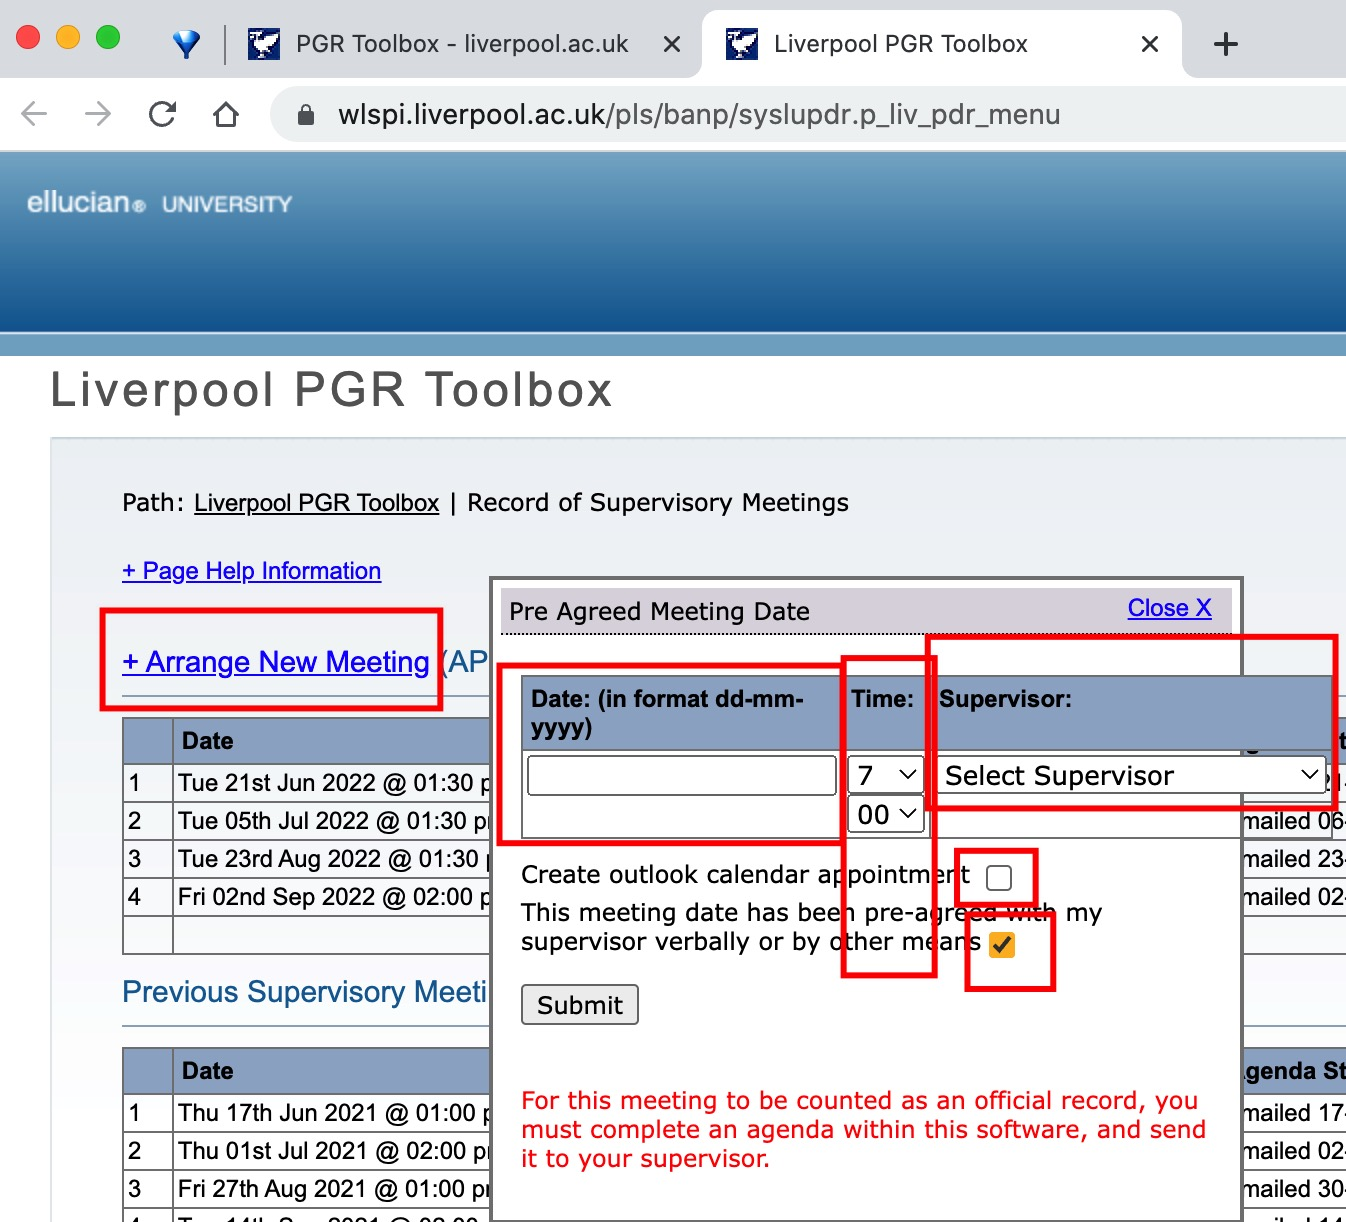
\includegraphics[width=0.5\columnwidth]{author-folder/Kai.Wu/meeting_record_figures/arange_new_meeting.jpg}
    \end{figure}
    \item Then recall what you discussed in your most recent meeting with your supervisor and fill in the progress report (what you have done), targets (what you plan to do before the next meeting), and discussion items.
    \begin{figure}[H]
        \centering
        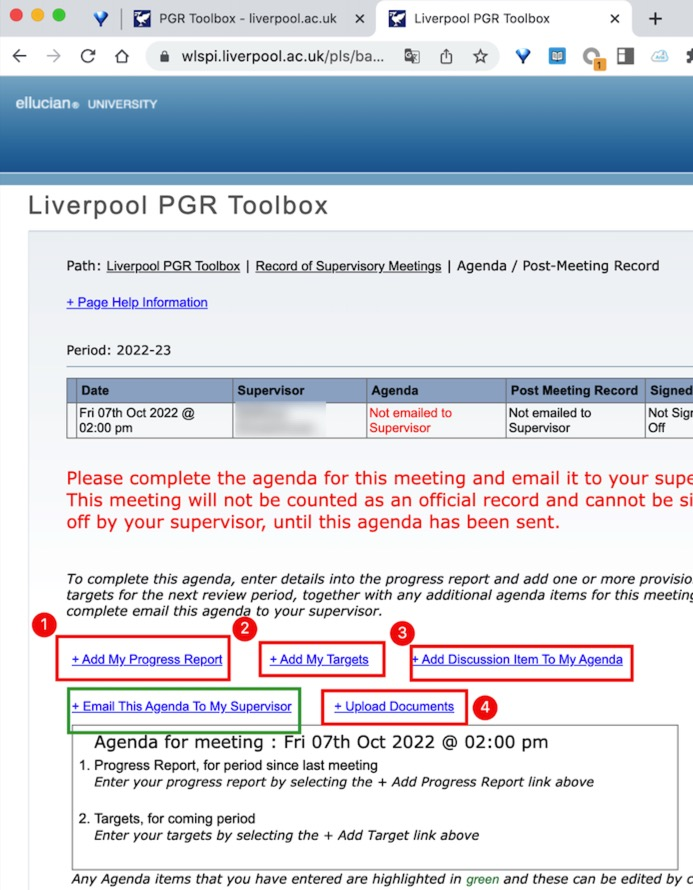
\includegraphics[width=0.5\columnwidth]{author-folder/Kai.Wu/meeting_record_figures/add_items_to_meetings.jpg}
    \end{figure}
    \item The content doesn't need to be extensive, but it shouldn't be too perfunctory either, as Liverpool will check it. After completing it, click "email this agenda", and both you and your supervisor will receive an automatically generated email in your Liverpool inboxes.
    \begin{figure}[H]
        \centering
        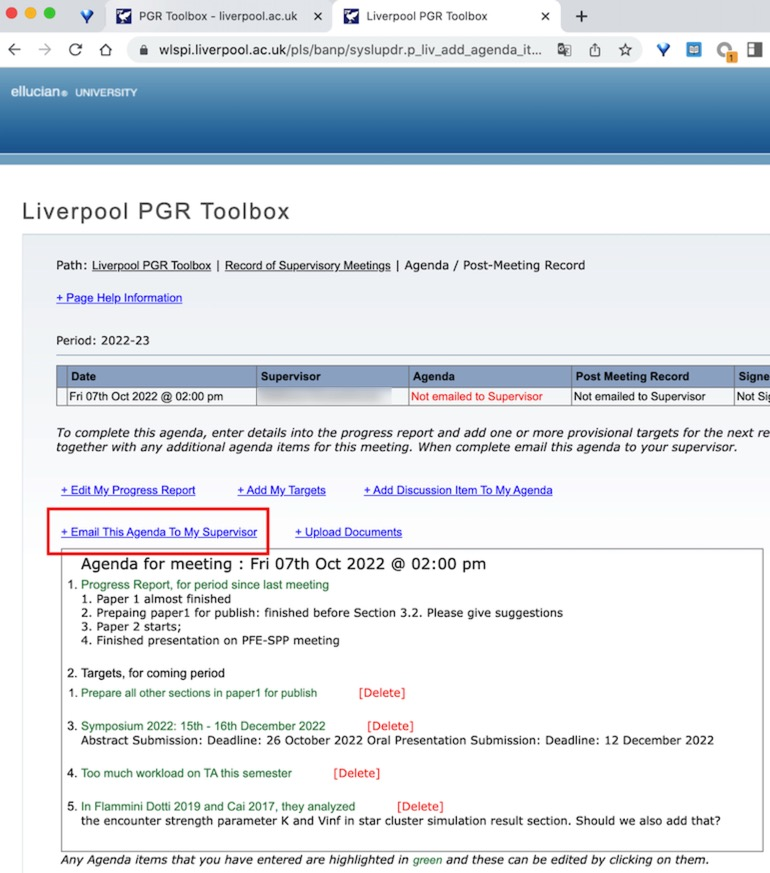
\includegraphics[width=0.5\columnwidth]{author-folder/Kai.Wu/meeting_record_figures/email_to.jpg}
    \end{figure}
    \item Don't be in a hurry to close it yet; you still need to fill in the comments from your meeting. Click "view edit meeting" on the right.
    \begin{figure}[H]
        \centering
        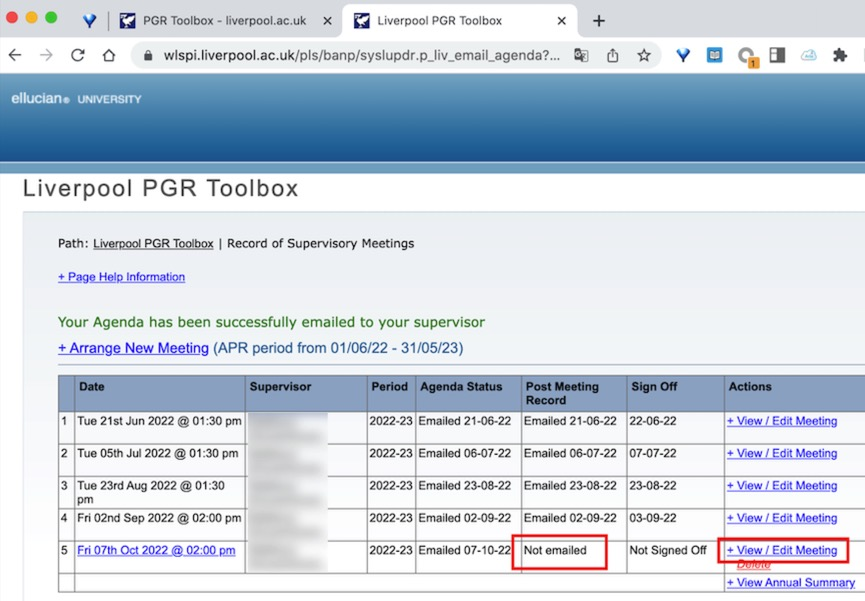
\includegraphics[width=0.5\columnwidth]{author-folder/Kai.Wu/meeting_record_figures/view_edit.jpg}
    \end{figure}
    \item Enter the comments from the meeting. Finally, click "email" at the top left, and you and your supervisor will receive another email in your Liverpool inboxes.
    \begin{figure}[H]
        \centering
        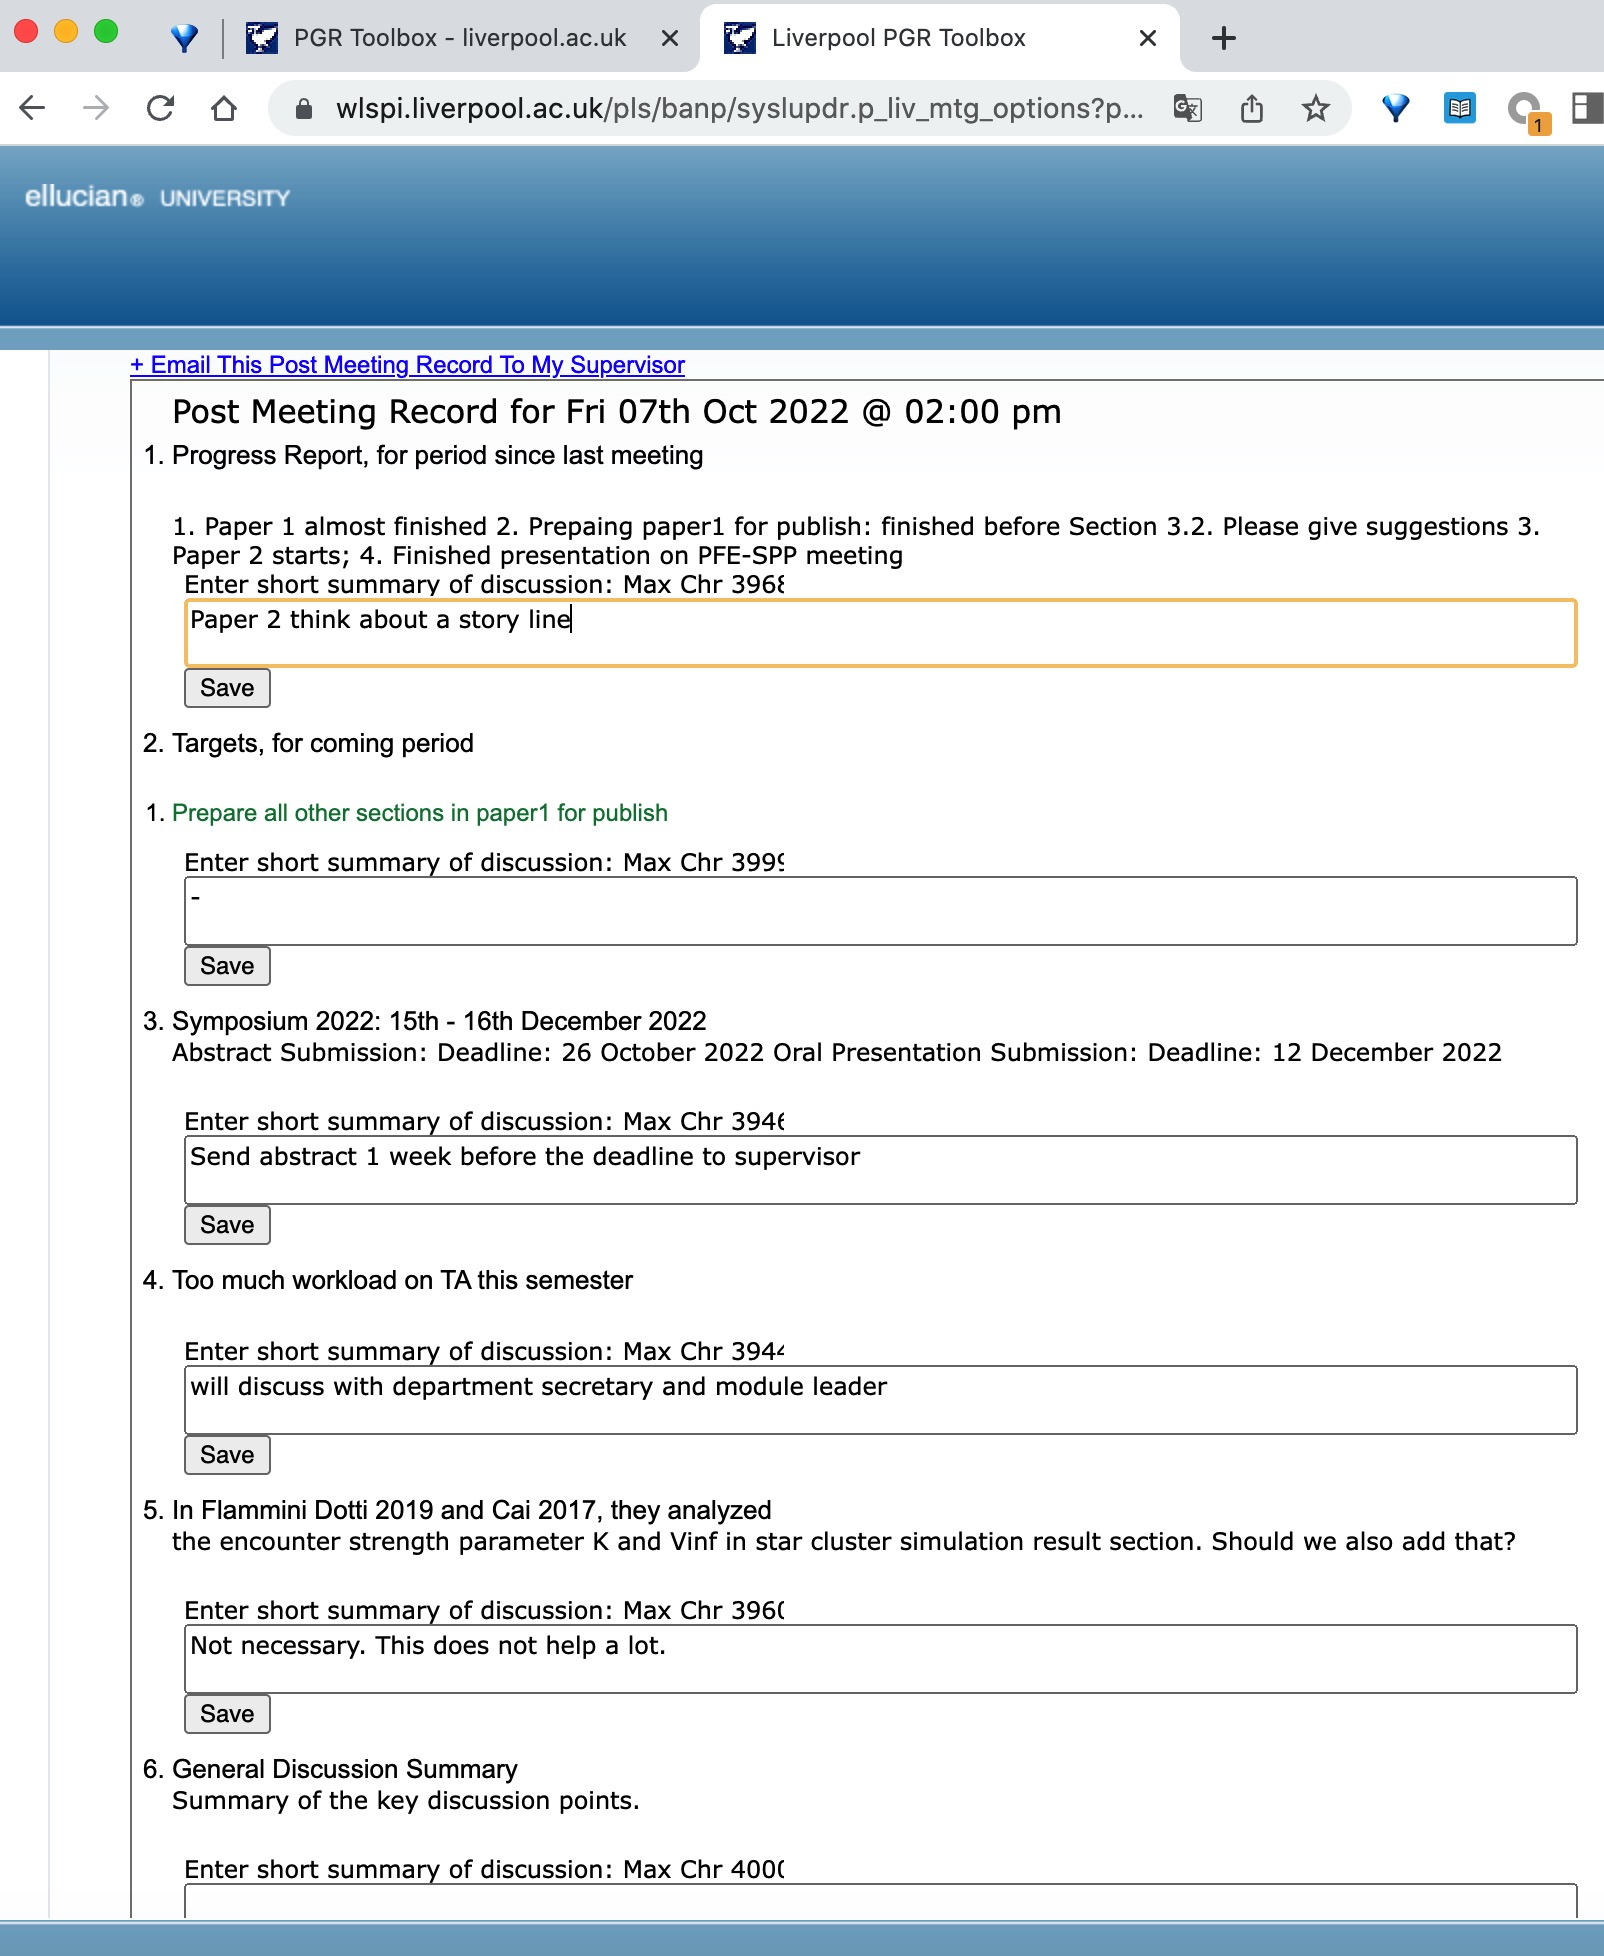
\includegraphics[width=0.5\columnwidth]{author-folder/Kai.Wu/meeting_record_figures/post_meeting.jpg}
    \end{figure}
    % \item 
    %     \begin{minipage}{0.3\textwidth}
    %         Due to the quirks of Liverpool Life, it is recommended to manually log out by clicking the top right corner in the Liverpool Life interface; otherwise, it may be difficult to log in next time.
    %     \end{minipage}
    %     \begin{minipage}{0.7\textwidth}
    %         \begin{figure}[H]
    %             \centering
    %             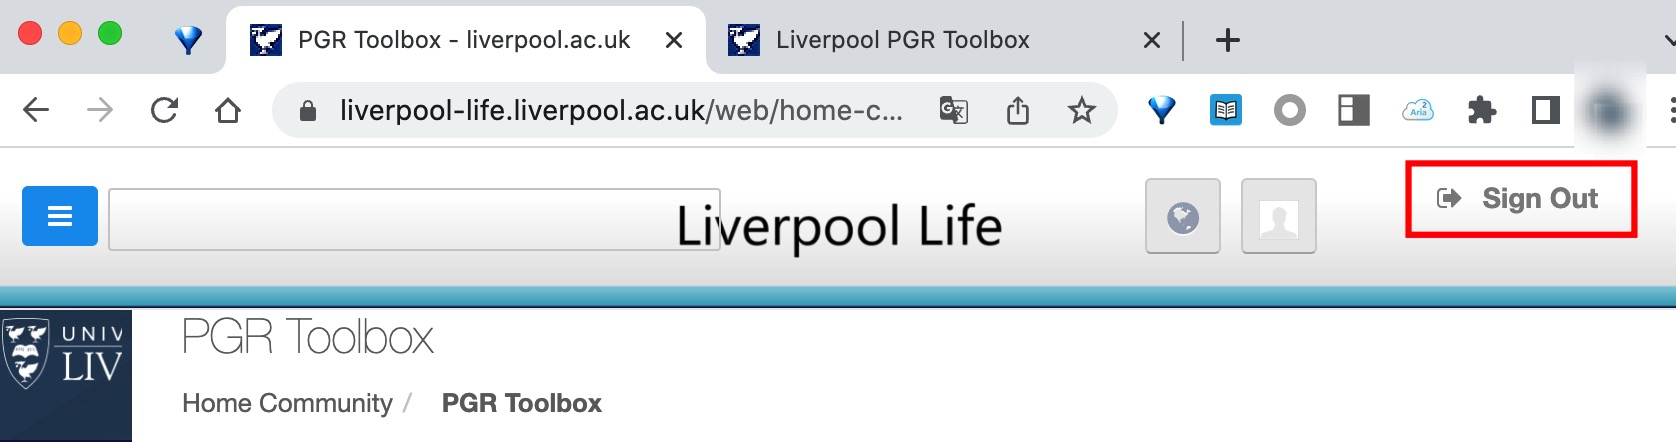
\includegraphics[width=0.9\columnwidth]{author-folder/Kai.Wu/meeting_record_figures/sign_out.jpg}
    %         \end{figure}
    %     \end{minipage}
    % \begin{figure}[H]
    %     \centering
    %     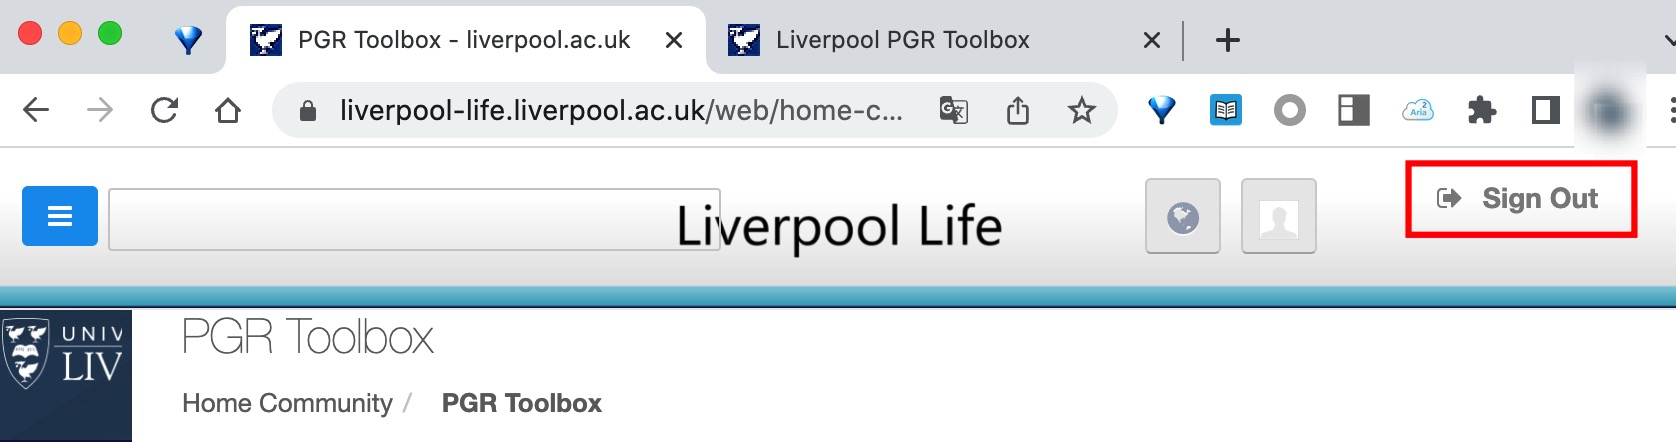
\includegraphics[width=0.5\columnwidth]{author-folder/Kai.Wu/meeting_record_figures/sign_out.jpg}
    % \end{figure}
    \item At this point, you're finished. Your supervisor needs to click "sign off" in the email they received in their Liverpool inbox. Afterwards, your Liverpool inbox will receive an email titled \textit{PGR Supervisor Meeting 5 (Fri 07th Oct 2022 @ 02:00 pm): sign off comments}, and this meeting record is then considered complete. Before each year's APR, all monthly meetings must be signed off at least once a month. If your supervisor hasn't signed off, you need to remind them.
\end{enumerate}

\vspace{5mm}
[Several Notes]
\begin{itemize}
    \item It's best to fill out this record once a month. Although you can make it up later — that is, not filling it out for several months and then filling in half a year's worth at once — is allowed, it's not standard practice. From my personal experience, if you wait until just before the APR to make it up, you'll either forget your progress over the year, or be too busy during the APR period. So, try to fill it out monthly as required.
    \item Liverpool Life and this reporting website often cannot be accessed! Due to various network and system issues, even using Wi-Fi and wired connections on the XJTLU campus, access is hit or miss. According to fellow students' experiences, using a VPN with a global proxy greatly improves connectivity, but such methods are not entirely legal and should not be taught to others, and absolutely should not be discussed on WeChat or QQ; otherwise, accounts may be blocked or groups may be banned. Students who cannot use VPNs should try to fill out the report early; otherwise, not being able to log in before the deadline will cause more anxiety.
\end{itemize}

\begin{flushright}
    October 10, 2022 by \Wu \\
    GPT translation proofread by \Shiyao
    \end{flushright} \clearpage

\section{APR}
\subsection{What is APR}
Firstly, please read the official description. If you haven't read it, please make sure to read every word carefully, because the importance of APR is equivalent to a small defense. If you fail, you may be expelled.

\url{https://www.liverpool.ac.uk/student-administration/research-students/progression/annual-progress/}

In my understanding, the purpose of APR is
\begin{itemize}
    \item Interview: Pursuing a PhD is not easy, so the university and the school need to understand the problems students encounter and help solve them.
    \item Seminar: Exercise presentation skills and get to know other PhD students.
    \item Progress report: Check student progress, further discover and help solve problems students encounter. At the same time, screen out students who are not studying seriously at all.
\end{itemize}

Some students may feel nervous when facing APR for the first time. In fact, as long as you haven't been idling away for the entire year—reading books, reading literature, writing articles, doing surveys, conducting experiments, writing code, etc.—the reviewers will not make things difficult for you and won't fail you. It is said that in 2022, a student in a certain school failed the APR. According to reliable sources, this person almost disappeared from human society, didn't reply to the supervisor at all, and didn't do any work, which is why they failed.

Also, note that another main function of APR is to help everyone solve problems. Therefore, you should boldly expose your problems in the APR and seek help (Chapter \ref{sec.IPAP}).

\subsection{APR Process}
\subsubsection{Preparation Work}
The pre-requisite task for APR is only one, which is to fill in the meeting records at least once a month. For how to fill out the meeting records, refer to Section \ref{sec.meeting_record}.

Then, each year there are two important emails about APR:
\begin{enumerate}
    \item 
        \begin{minipage}{0.3\textwidth}
            The first is an email sent by XJTLU in May, which looks like this, sent to your XJTLU email.
        \end{minipage}
        \begin{minipage}{0.63\textwidth}
            \begin{figure}[H]
                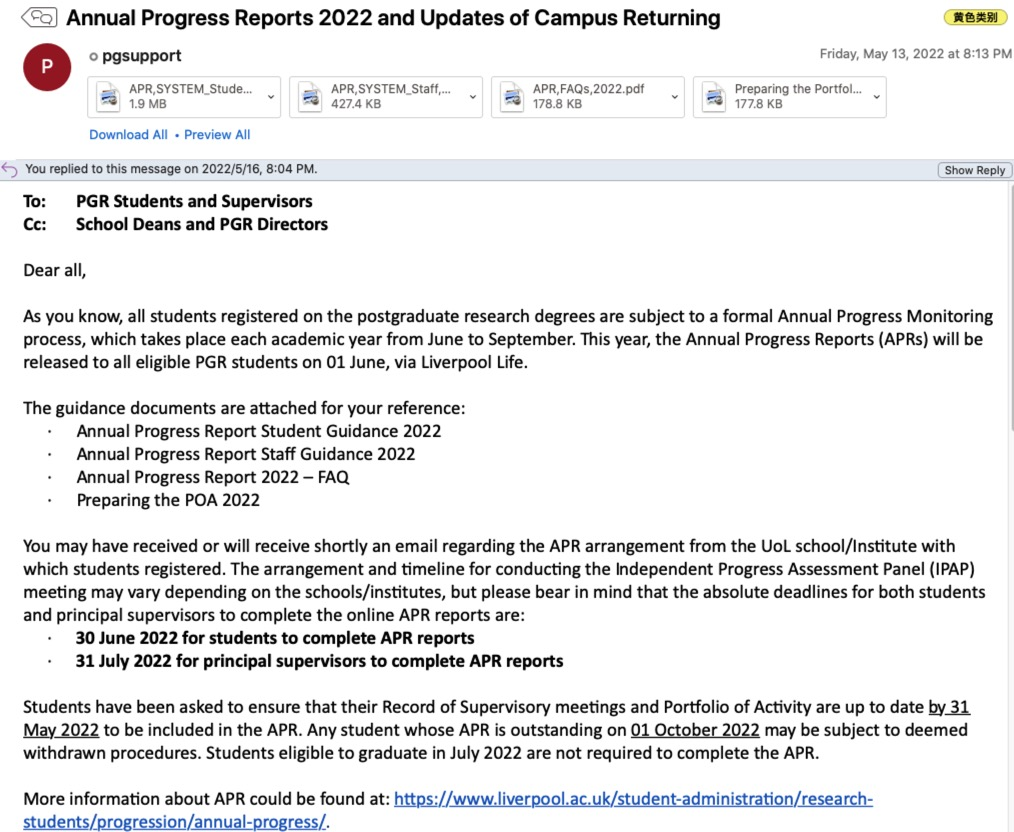
\includegraphics[width=0.95\columnwidth, right]{author-folder/Kai.Wu/APR_email.jpg}
            \end{figure}
        \end{minipage}

    \item 
        \begin{minipage}{0.3\textwidth}
            The second is an email sent by your University of Liverpool school between April and May. For the Mathematics school, it looks like this and is sent to your Liverpool email. Other schools may be different. The time when each school sends the notification also varies greatly, some as early as April, some delayed until the end of May.
        \end{minipage}
        \begin{minipage}{0.63\textwidth}
            \begin{figure}[H]
                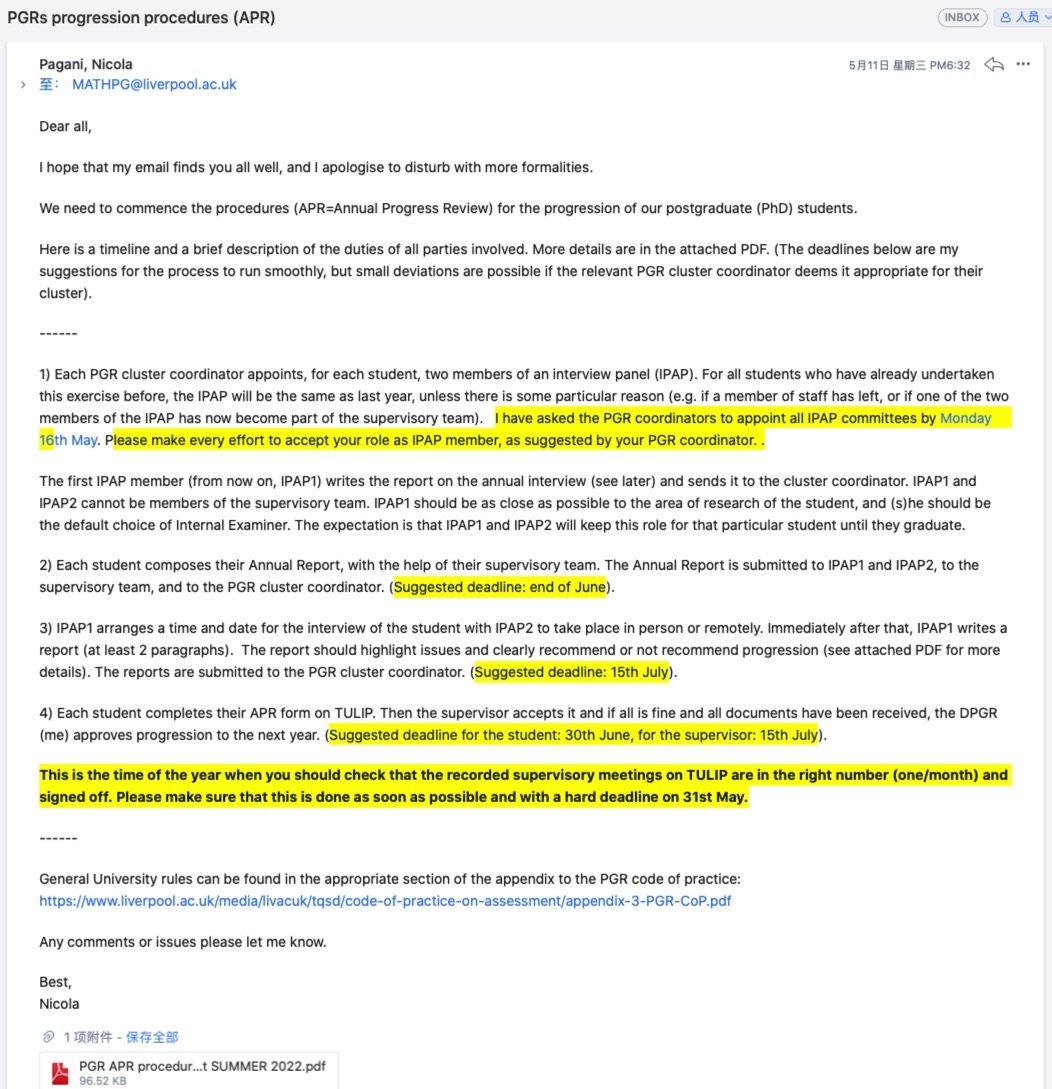
\includegraphics[width=0.95\columnwidth, right]{author-folder/Kai.Wu/APR_liverpool_email.jpg}
            \end{figure}
        \end{minipage}

\end{enumerate}

The APR requirements of each school are slightly different, so around May, please be sure to check your Liverpool email. Read both emails carefully. For students doing APR for the first time, it is recommended to read the two emails and attachments word by word.

The specific content of APR includes the following four parts:

\subsubsection{TULIP Web Form}
What the Liverpool and XJTLU emails refer to as "Your annual progress report has been released" means that you can fill in this green form. The main parts to fill in are:
\begin{enumerate}
    \item SUMMARY OF PROGRESS: Progress report, above 300 words, below 4000 characters (about 600 words).
    \item Seminars and Conference attendance, Library and IT training and all subject-specific training including research methods and experimental techniques. (Recall, the more the better, if you really have none, it's okay.) Seminars, conferences, professional skills training you've attended.
    \item Attendance at careers events and workshops covering Employability and Entrepreneurship and including attendance at any other Professional development workshops. (The more the better.) Career-related activities you have attended.
    \item Training and completion of activities relating to Health and Safety, ethics, grant writing, and similar activities, including Project Management. (The more the better.) Activities not directly related to study but relevant.
    \item Details of your presentations, written publications, teaching and public engagement/impact activities, and related training for these activities. (The more the better.) Presentations, published papers, teaching assistant work you've done.
    \item PERSONAL OR ACADEMIC PROBLEMS: Have there been any problems in the last year which you feel have affected your progress? (Fill in according to the actual situation.) Have you encountered any problems that hindered your studies. You can sincerely raise problems, or appropriately explain, such as "My progress is insufficient because of xxxxx (illness/marriage/poor school network/slow English reading/insufficient ability in certain aspects)."
\end{enumerate}

\begin{figure}[H]
    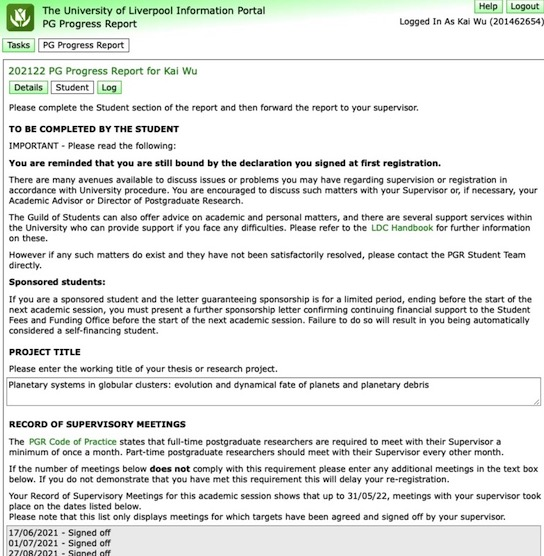
\includegraphics[width=0.7\columnwidth, center]{author-folder/Kai.Wu/TULIP.jpg}
\end{figure}

All students are required to fill in the TULIP form regardless of the school. But the following three parts may have very different requirements for each school, and also partially depend on the University of Liverpool school you belong to. You might want to double-check with your seniors.

\subsubsection{Annual Report (AR)}
In short, write a document about what you've done. There might be word or page requirements. If you really don't know what to write, I personally suggest you can write everything in detail (like a diary), for example, what literature you read and what you gained; what code you wrote or experiments you did. Importantly, what academic activities you've participated in, such as conferences, meetings, and being a teaching assistant, can all be included. In other words, just repeat the content of the TULIP form in the document, basically copy and paste, and if the word count is insufficient, expand the content.

Of course, if there are special requirements, follow them. For example, the Mathematics school requires Year 3 students to submit a Thesis Outline, so you don't need to write a diary.

Please note that this description of the AR part is based on my own experience in the School of Mathematics and Physics. According to other students, many schools have similar requirements, but some schools require much more. According to a chemistry student, they had to write a 30-50 page literature review in the first year, which must be prepared one or two months in advance. New students must consult your seniors or supervisors.

\subsubsection{Annual Seminar}
Generally, all PhD students in a school or department are gathered to do presentations, give each other feedback, and get to know each other. As far as I know, some departments with fewer people skipped this part or merged it into the interview below, turning it into a presentation to two teachers. In any case, you need to prepare a \textbf{PPT} to let others understand your research. You can prepare for a 20-minute presentation plus a 5-minute Q\&A session; some schools may have different requirements, so ask seniors. If you have a lot of research results, you can highlight them; if not, you can present what you've done like a diary to fill the time, making the teachers feel you've done a lot of work.

\subsubsection{IPAP Interview}
\label{sec.IPAP}
The school will find two teachers who are not your supervisors and have no conflict of interest with you to have a face-to-face talk. You may need to prepare a \textbf{PPT} and confidently include your issues in it. All the following problems can be discussed with the IPAP teachers. According to the requirements, the two teachers will do their utmost to help you solve problems:
\begin{itemize}
    \item Equipment problems: School computer malfunctions, such as inconvenient use, lagging, crashes; office environment problems (e.g., air conditioning blowing directly on your head).
    \item Real research problems: You've read too few papers and don't know how to read efficiently; you don't know experimental methods; you have great difficulties in writing; due to non-subjective reasons, you cannot attend many academic meetings (for example, in recent years, every year during APR we complain about various impacts of the pandemic), etc.
    \item Supervisor problems: Your supervisor exploits you, making you work excessively every day, leaving you exhausted; your supervisor makes you do a lot of unrelated work, such as moving house for them, getting takeout, handling reimbursements; your supervisor is very harsh on you, pressuring you, making you highly stressed every day; your supervisor frequently calls, sends messages, or emails outside of work hours and asks you to respond immediately, leaving you no rest; your supervisor takes the first authorship of your paper; your supervisor is often unavailable, not replying to your emails for several days. These problems are serious derelictions of duty by the supervisor. Once encountered, they can cause severe psychological burdens and affect future work efficiency. IPAP is here to address this, so be sure to discuss it clearly with the interviewing teachers.
    \item Emotional and psychological problems: Anxiety, nervousness, insomnia, depressive tendencies (Note: If you feel you are not in a good state, please contact the school's counseling center at \email{counsellingservice@xjtlu.edu.cn} as soon as possible; it's free).
    \item Family pressure: Your family expects you to graduate in 3 years, but you feel too much pressure.
    \item Financial pressure, health problems (serious discomfort that may require you to suspend or take leave to recuperate), any problems that affect your normal PhD work.
\end{itemize}

\vspace{5mm}
Identifying and solving all problems, then starting the next academic year, is the main purpose of APR. If there are any problems that APR cannot conveniently address or solve, please communicate with your supervisor, department head, dean, your DA, or the school's counseling center in time. Also, please refer to Chapter \ref{sec.mental_health} "Pay Attention to Your Negative Emotions and Depressive Tendencies" in this manual.

\begin{flushright}
(October 12, 2022 by \Wu) \\
(Translated by GPT)
\end{flushright} \clearpage

\section{Research Symposium}

\subsection{What is XPGRS}
XJTLU Postgraduate Research Symposium, abbreviated as XPGRS or Symposium, is an event organized by the Graduate School. Every year, commonly December, all PhD students in the university are invited to present their research results or progress through posters or oral presentations. Each year's XPGRS is announced via email around October.

\subsection{Which event do I need to participate in?}

The official requirements are as follows:

\begin{itemize}
    \item Second-year PhD students need to give poster presentations
    \item Third-year PhD students need to give oral presentations
    \item Fourth-year or above PhD students will be invited to serve as session chairs
    \item Master's students in the dissertation stage are also welcome to participate
\end{itemize}

Based on past experiences, this translates to:

\begin{itemize}
    \item First-year students have nothing required, but can consider volunteering (an email will be sent for recruitment) or simply attend to observe and learn about seniors' work
    \item Second-year students must do a poster
    \item Third-year students must give an oral presentation and may consider being a chair
    \item Fourth-year or above students are free to choose
\end{itemize}

To determine which year you are in, use December 1st of the current year as the reference. This is straightforward for those who enrolled between March and September, but many students happen to enroll on December 1st. According to the 2022 information, these students are required to participate, meaning, for example, if you enrolled in December 2021, you need to do a poster in 2022.
% These students can choose whether to participate after one year. For example:
% \begin{itemize}
%     \item Student A enrolled in December 2020. In December 2021, he found he had too little to show and decided not to participate. Therefore, he must do a poster in December 2022, an oral presentation in December 2023, and is free in December 2024.
%     \item Student B enrolled in December 2020. In December 2021, she felt she could present something and wanted to improve her skills early, also as preparation for future academic conferences. So she participated in the poster session in December 2021, then had to give an oral presentation in December 2022, and is free in December 2023.
% \end{itemize}
%
Of course, since December entrants are special cases, policies may change, so it's best to email (or call) the Graduate School each year to inquire.

Theoretically, you can participate in both poster and oral sessions every year if you wish! You can even choose not to participate at all, but you need your supervisor's approval. Generally, unless there's a special reason, supervisors hope you can gain experience. If there is a valid reason, your supervisor can contact the Graduate School, and with their agreement, you can opt out. (I've heard of supervisors who think the symposium is useless and have their students never participate, and some who have students do both poster and oral presentations from the start...)

\begin{figure}[H]
    \caption{Poster session of the 2021 Symposium (CB G13W), before the official start}
    \centering
    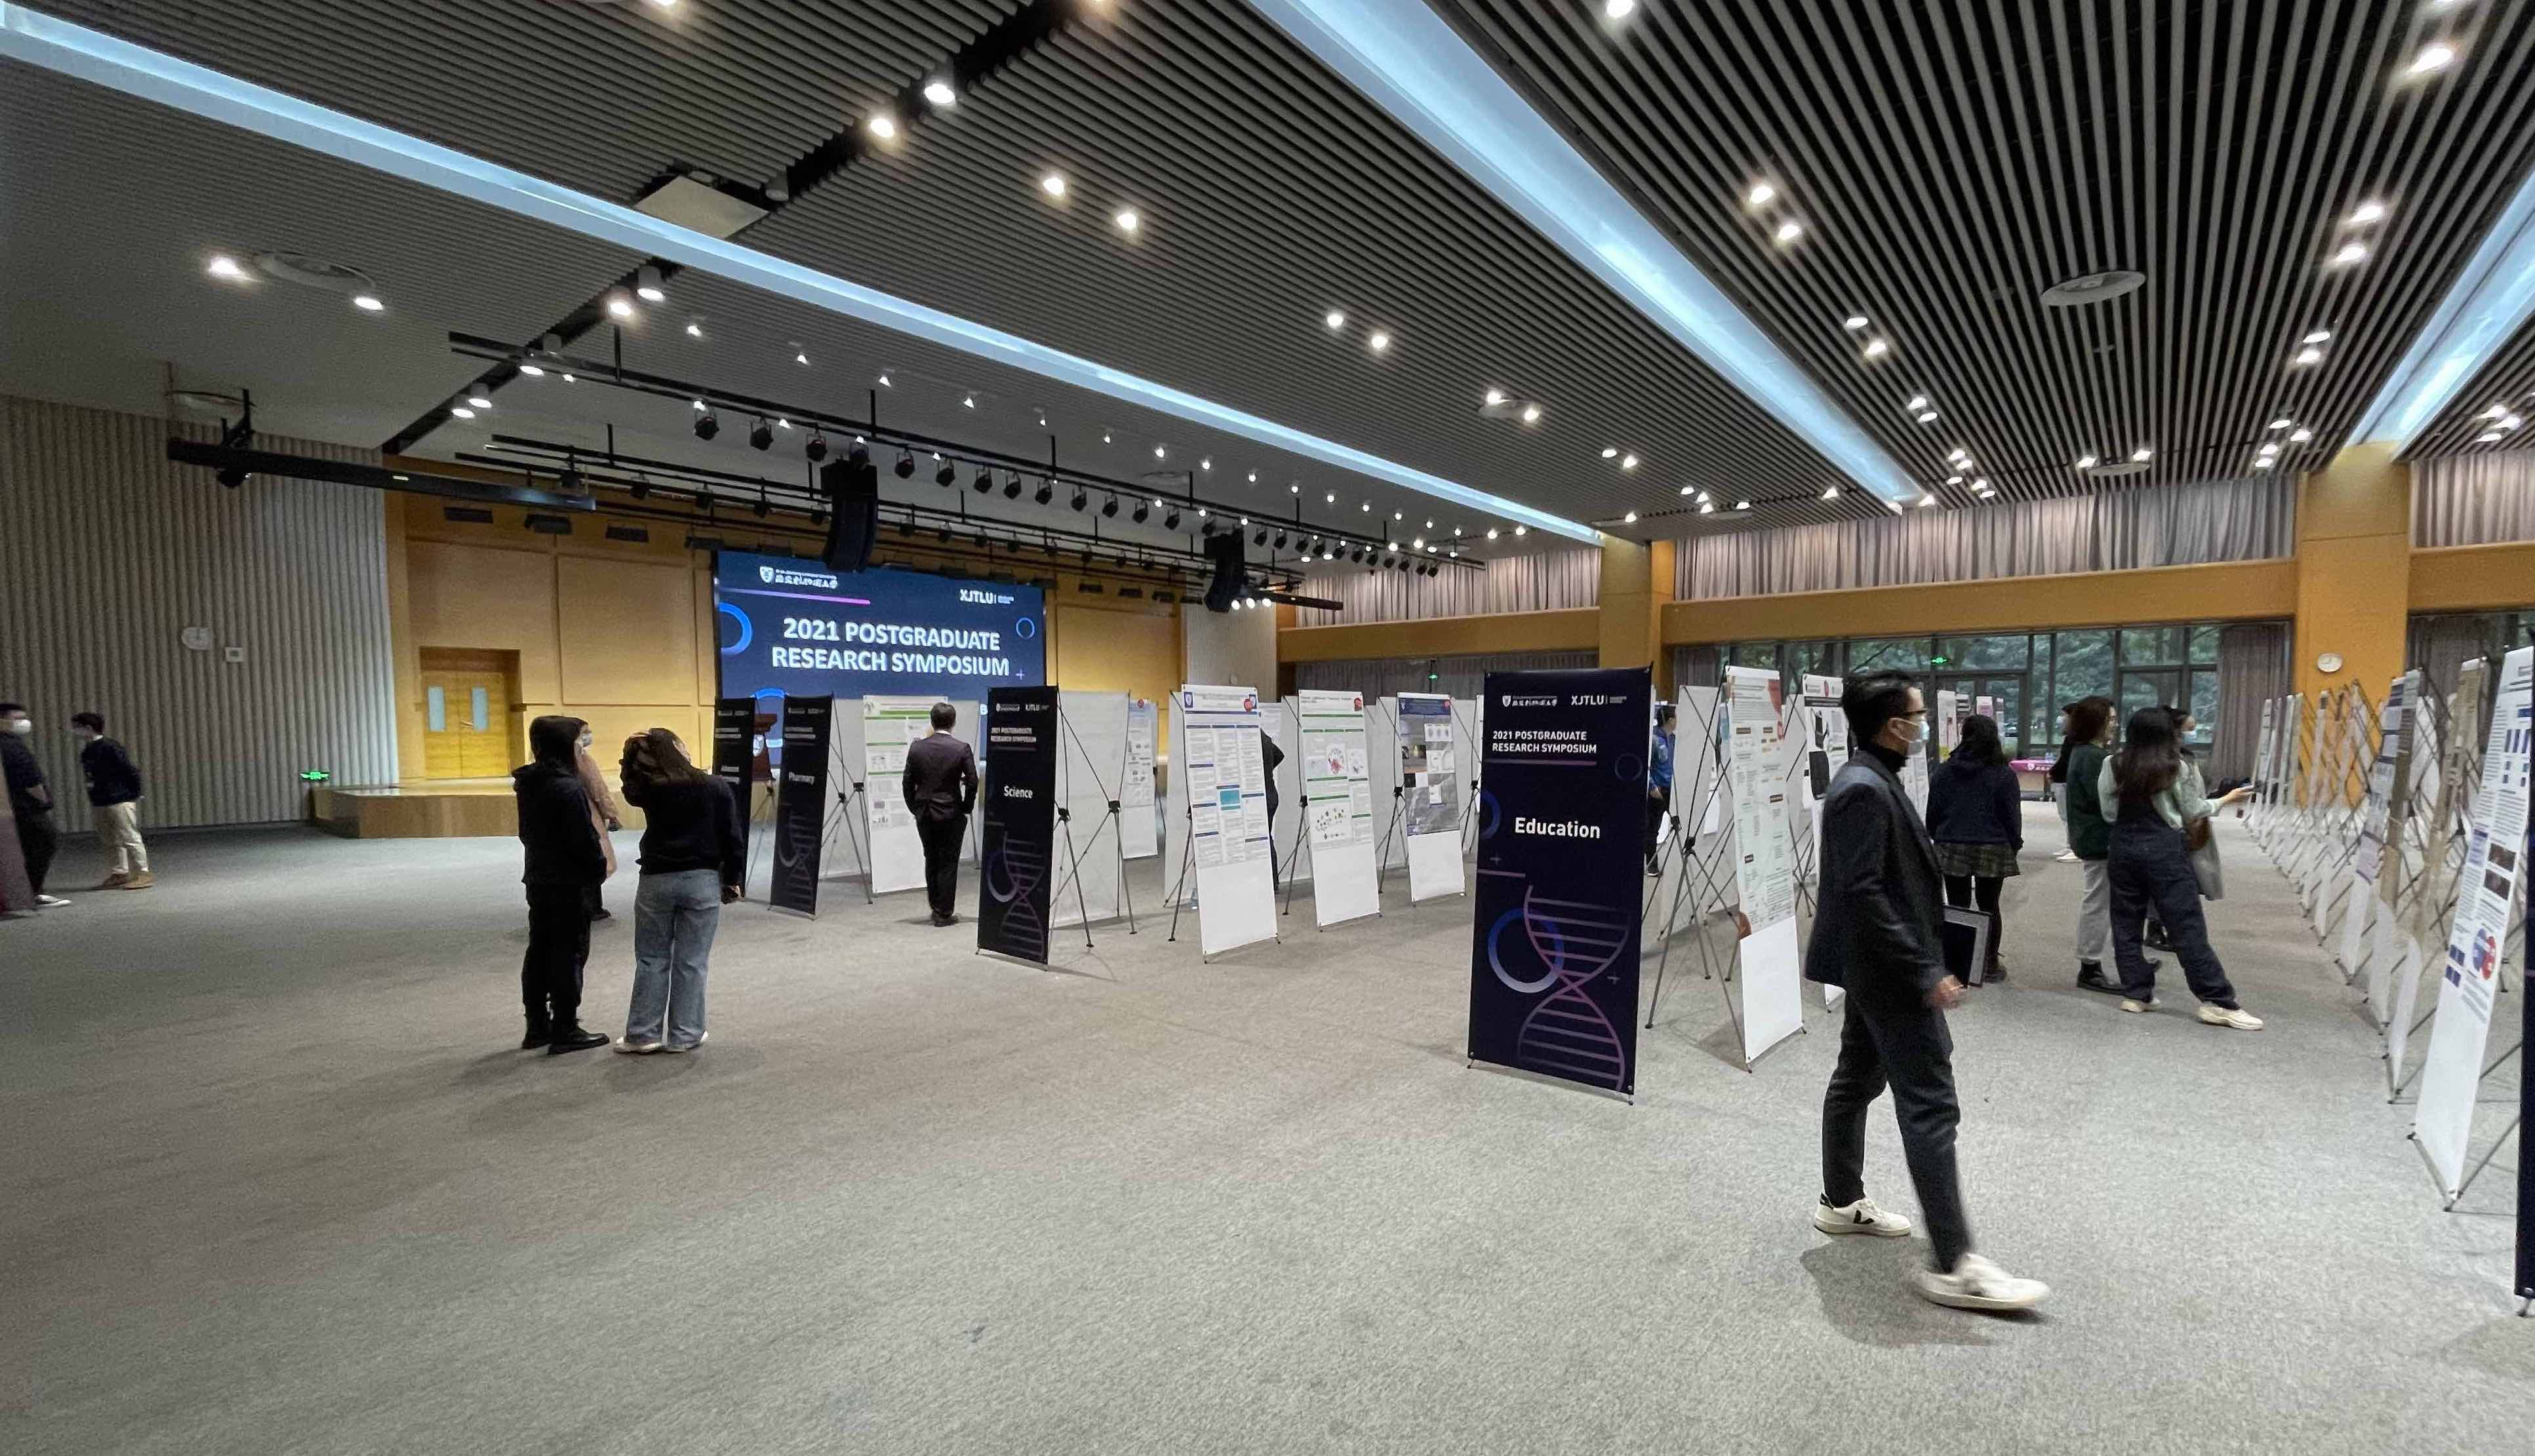
\includegraphics[width=\columnwidth]{author-folder/Kai.Wu/synposium_poster.jpg}
\end{figure}

\subsection{What are the benefits?}

\begin{enumerate}
    \item Improve presentation skills, practice English speaking, and receive guidance from other faculty members
    \item Opportunity to win awards. The university will invite several faculty members to listen to your poster or presentation and score you. Awards include Best Poster Award (10\%), Best Presentation Award (10\%), Excellent Poster Award (20\%), Excellent Presentation Award (20\%), with a certificate and conference funding of 1000 or 500 yuan (for usage of conference funding, see section \ref{sec.fund}). Although it's not a cash reward, it's still useful \sout{(stingy university)}
\end{enumerate}

\begin{figure}[H]
    \centering
    
\includegraphics[width=0.4\columnwidth]{author-folder/Kai.Wu/poster_award.jpg}
\end{figure}

\subsection{“I don't want to go”—Try not to!}

Some students often think: the rewards are minimal, the prestige is low, and even winning the best award isn't useful. Moreover, nothing happens if I don't go. Yes, frankly speaking, with your supervisor's consent, you can legally opt out; even if you simply disappear, there likely won't be consequences, and it's unrelated to graduation.

However, as someone who has participated in posters, oral presentations, chaired three oral sessions, and listened to many presentations, unless you are truly adept at giving presentations, I strongly recommend you participate! I've seen students reading scripts with their heads down the entire time, writing scripts directly on their PPTs and reading them, being overly nervous with trembling hands and voices, having PPTs that fail to distinguish primary and secondary points, or being at a loss when facing questions from faculty. Any of these issues would be fatal in your thesis defense!! Remember, our defense isn't a mere formality like at some universities; it's a real challenge where you must deliver a good presentation and answer every sharp question well. \textbf{Do you want to expose these problems during your defense, or discover them early, practice more, and resolve them sooner?}

Therefore, since in the Symposium you won't fail but only be evaluated, and the judges are friendly and will help you identify important issues, \uline{\textbf{it's a very safe and excellent opportunity for practice}}. You shouldn't wait until your defense or attending top conferences to start practicing!

\subsection{Notes and how to perform excellently}

Below is the oral presentation scoring sheet I saw at the 2022 Symposium (can be enlarged for viewing). The considerations for posters are quite similar (participants in the poster session also need to prepare a talk of about 3 minutes to introduce their work to the judges). Frankly speaking, these items are worth noting in any presentation and can be used to carefully review your poster.

\begin{figure}[H]
    \caption{Scoring sheets from 2022}
    \centering
    \begin{tabular}{rl}
        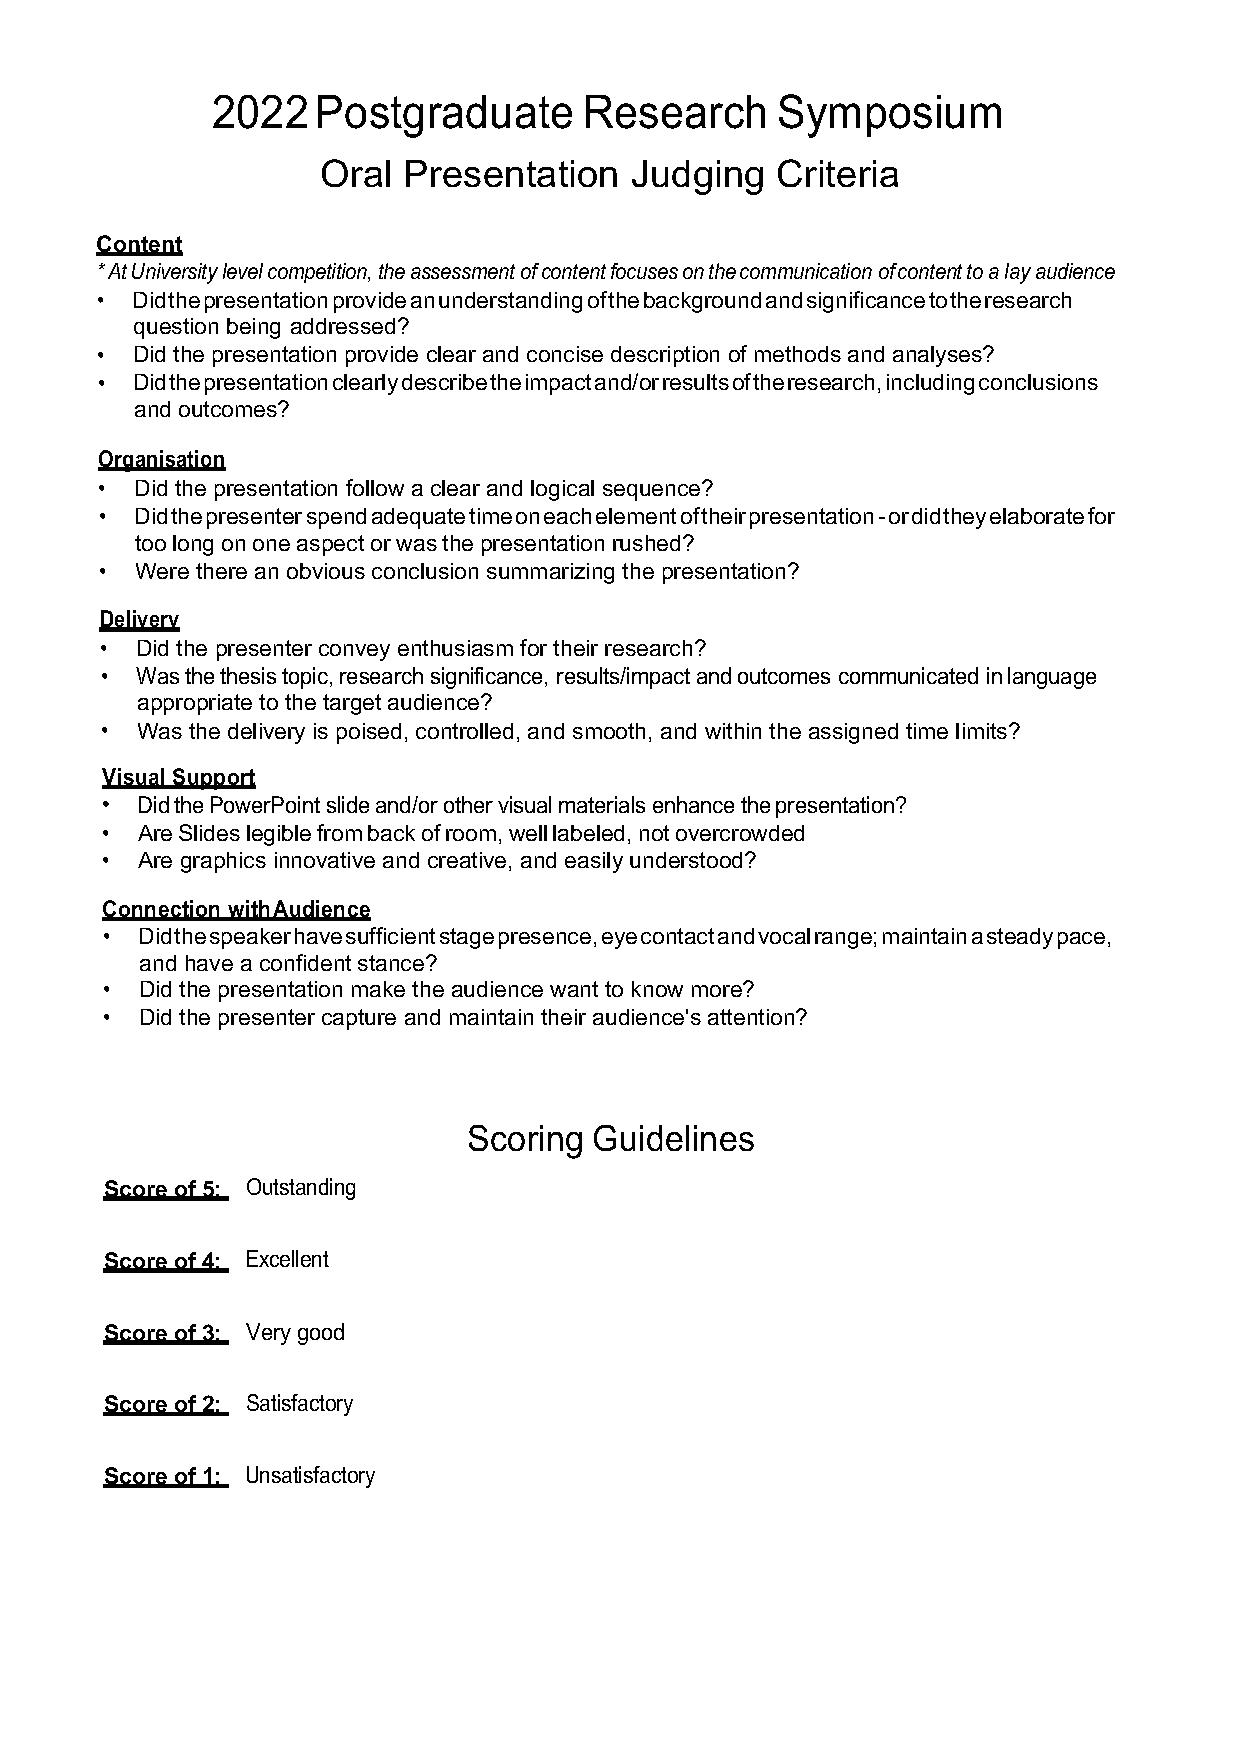
\includegraphics[width=0.5\columnwidth]{author-folder/Kai.Wu/2022_XPGRS_oral_judging_criteria.pdf} & 
        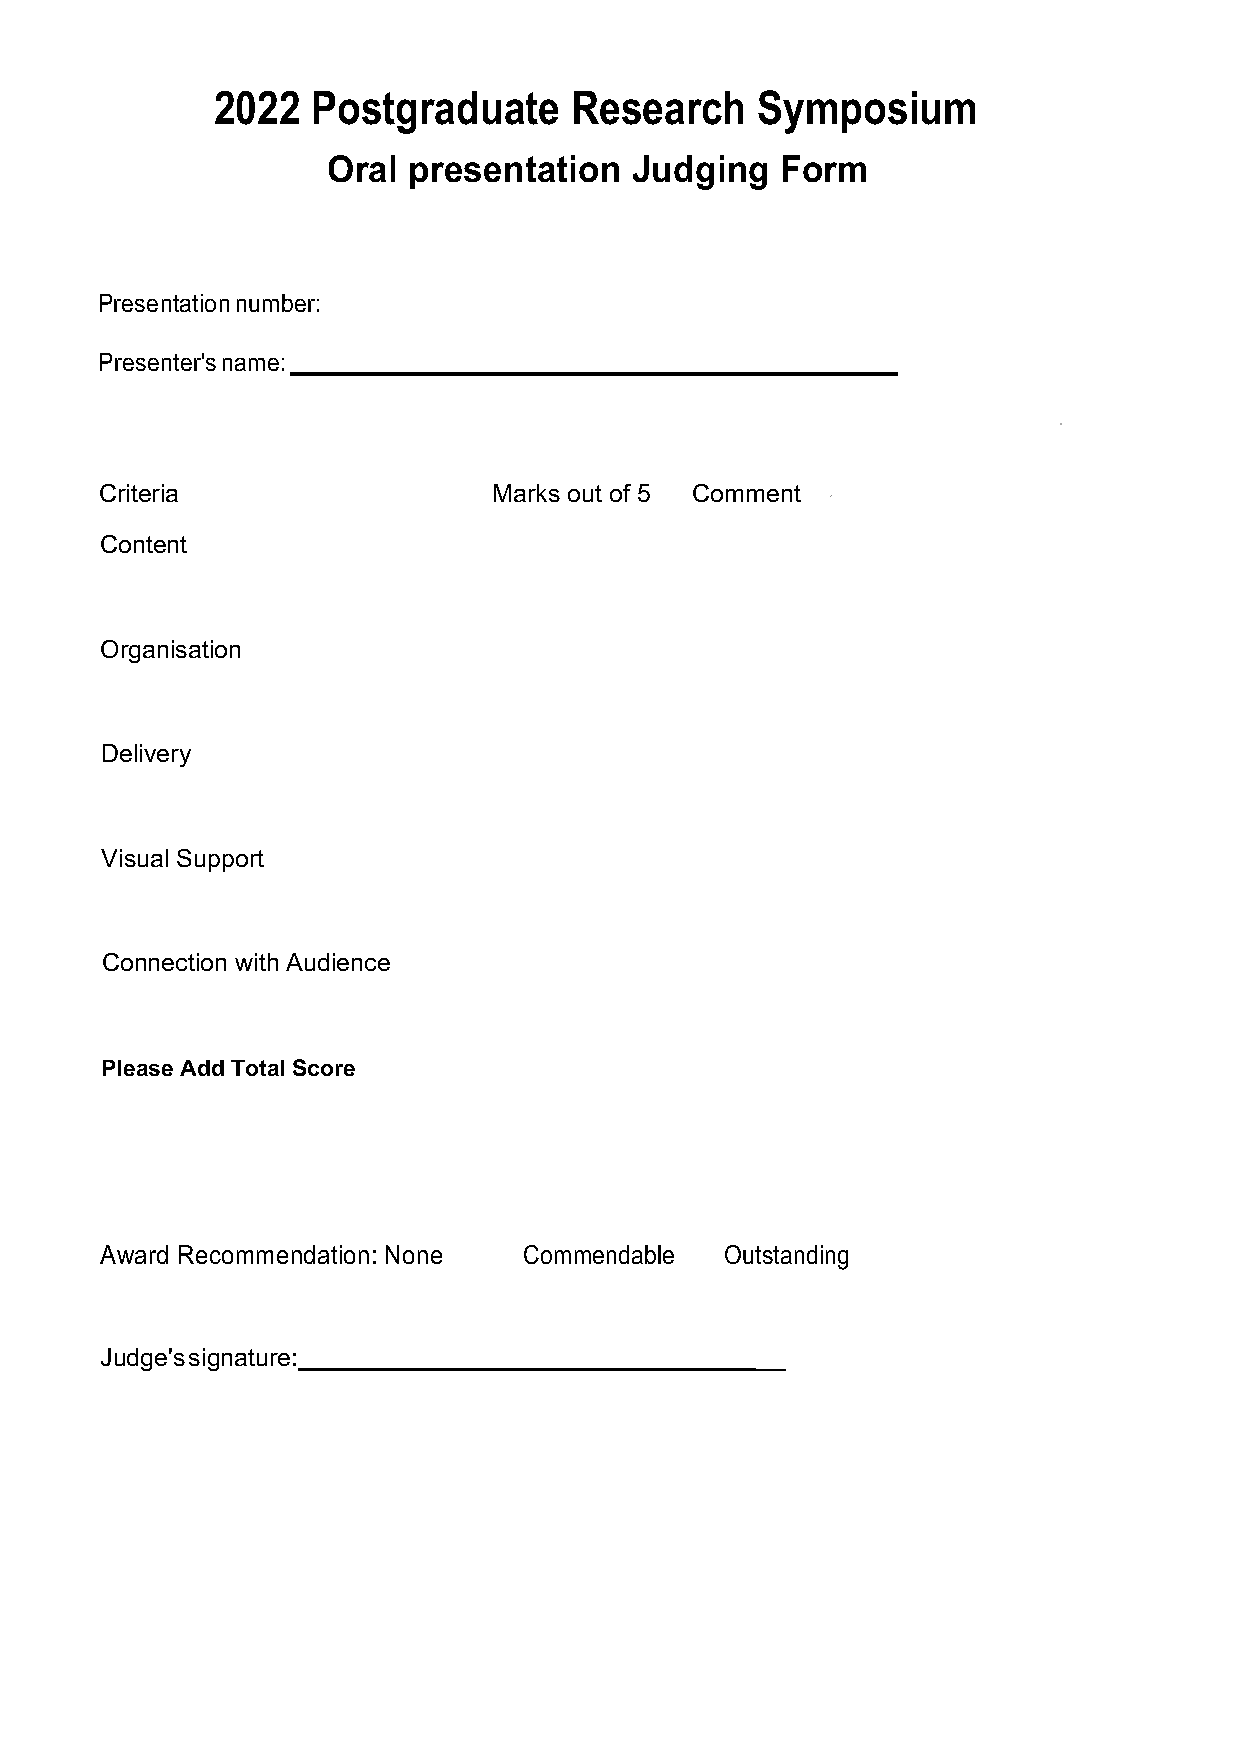
\includegraphics[width=0.5\columnwidth]{author-folder/Kai.Wu/2022_XPGRS_oral_judging_form.pdf} 
    \end{tabular}
\end{figure}

If you want to perform excellently and win awards, you can continue reading below:

There are plenty of tutorials online about giving presentations and making posters. However, the biggest difference between XPGRS and other academic presentations is that the vast majority of students, including the school's judges, may have absolutely no understanding of your research field (as they say, "each profession has its specialty"). If you present as you would to your supervisor, or simply reuse posters or PPTs from academic conferences full of experts, you might not win awards because the judges and other students simply don't understand.

My supervisor told me that XPGRS is different from academic presentations because it's geared toward non-specialists and is more like popular science. Part of the Symposium's goal is to see how you can make non-specialists interested in your research and understand about 70\% of it in a short time. If you're unsure how to do this, imagine one day you meet the Executive President Xi, our  in an elevator—how would you let him know what you're working on, its significance, and ideally pique his interest in a short time? Or, how would you explain your research to relatives or old classmates during the holidays? Academic research isn't done in isolation; being able to present your research and let your academic achievements benefit others is a very important skill.

\begin{flushright}
    October 19, 2022 by \Wu \\
    major update: December 16, 2022 by \Wu \\
    GPT translation proofread by \Shiyao
\end{flushright}


%# -*- coding: utf-8-unix -*-
%%==================================================

\chapter{Must-Read Information to Avoid Losses}
\label{fuli}

\section{会议经费}
\label{sec.fund}

每位同学,无论是自费生还是奖学金学生,都有16500元的会议经费。参加会议的时候,可以用来报销注册费、住宿交通等费用。这笔钱毕业前不用完拿去\sout{在会议周边吃喝玩乐出去浪}丰富自己的学术经历就亏啦。钱虽多,申请和报销流程比较繁琐。主要资料在:
\begin{itemize}
    \item e-bridge: \url{https://ebridge.xjtlu.edu.cn/},登陆过后点击PGR Policies, Procedures and Forms,找到 \textit{Postgraduate Research Students' Conference Fund Policy} 和 \textit{
    Guideline and Procedures on Doctoral Student Travel Arrangement and Reimbursement}
    \item 官方流程图
    \begin{figure}[H]
        \centering
        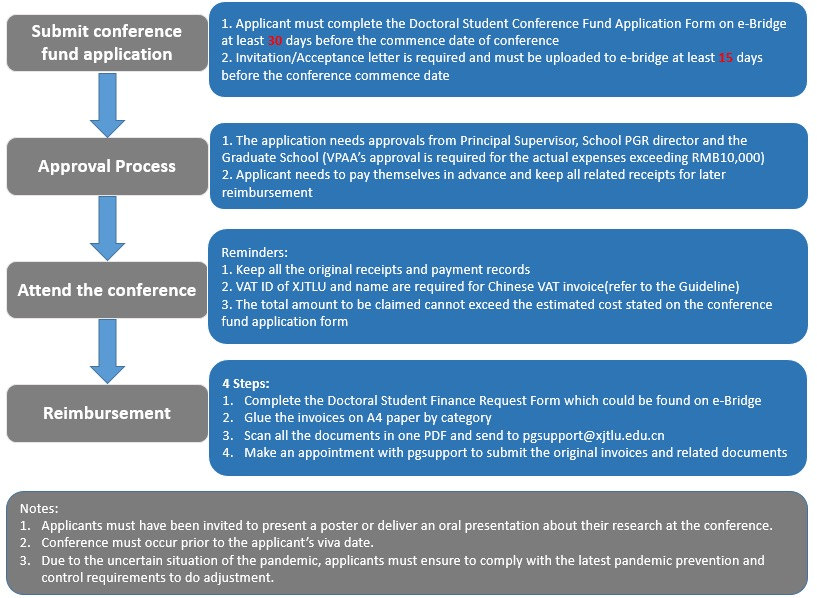
\includegraphics[width=0.9\columnwidth]{author-folder/Kai.Wu/fund-flowchart.jpg}
    \end{figure}
\end{itemize}

要注意
\begin{enumerate}
    \item 必须要至少提前30天申请。因此不能用于“你突然听说有个30天内要开的会议”
    \item 必须要在会议上作报告,poster或者oral都可以,否则不能使用经费
    \item 不能使用学校经费的时候,可能可以使用你导师的某些经费。我就因为上述原因,用导师的经费报销过几场会议。具体怎么做\&你导师到底有没有这种经费,问你自己的导师
\end{enumerate}


\begin{flushright}
(2022年10月12日 by \Wu)
\end{flushright}
\section{Free Stationaries}
\begin{figure}[H]
    \centering
    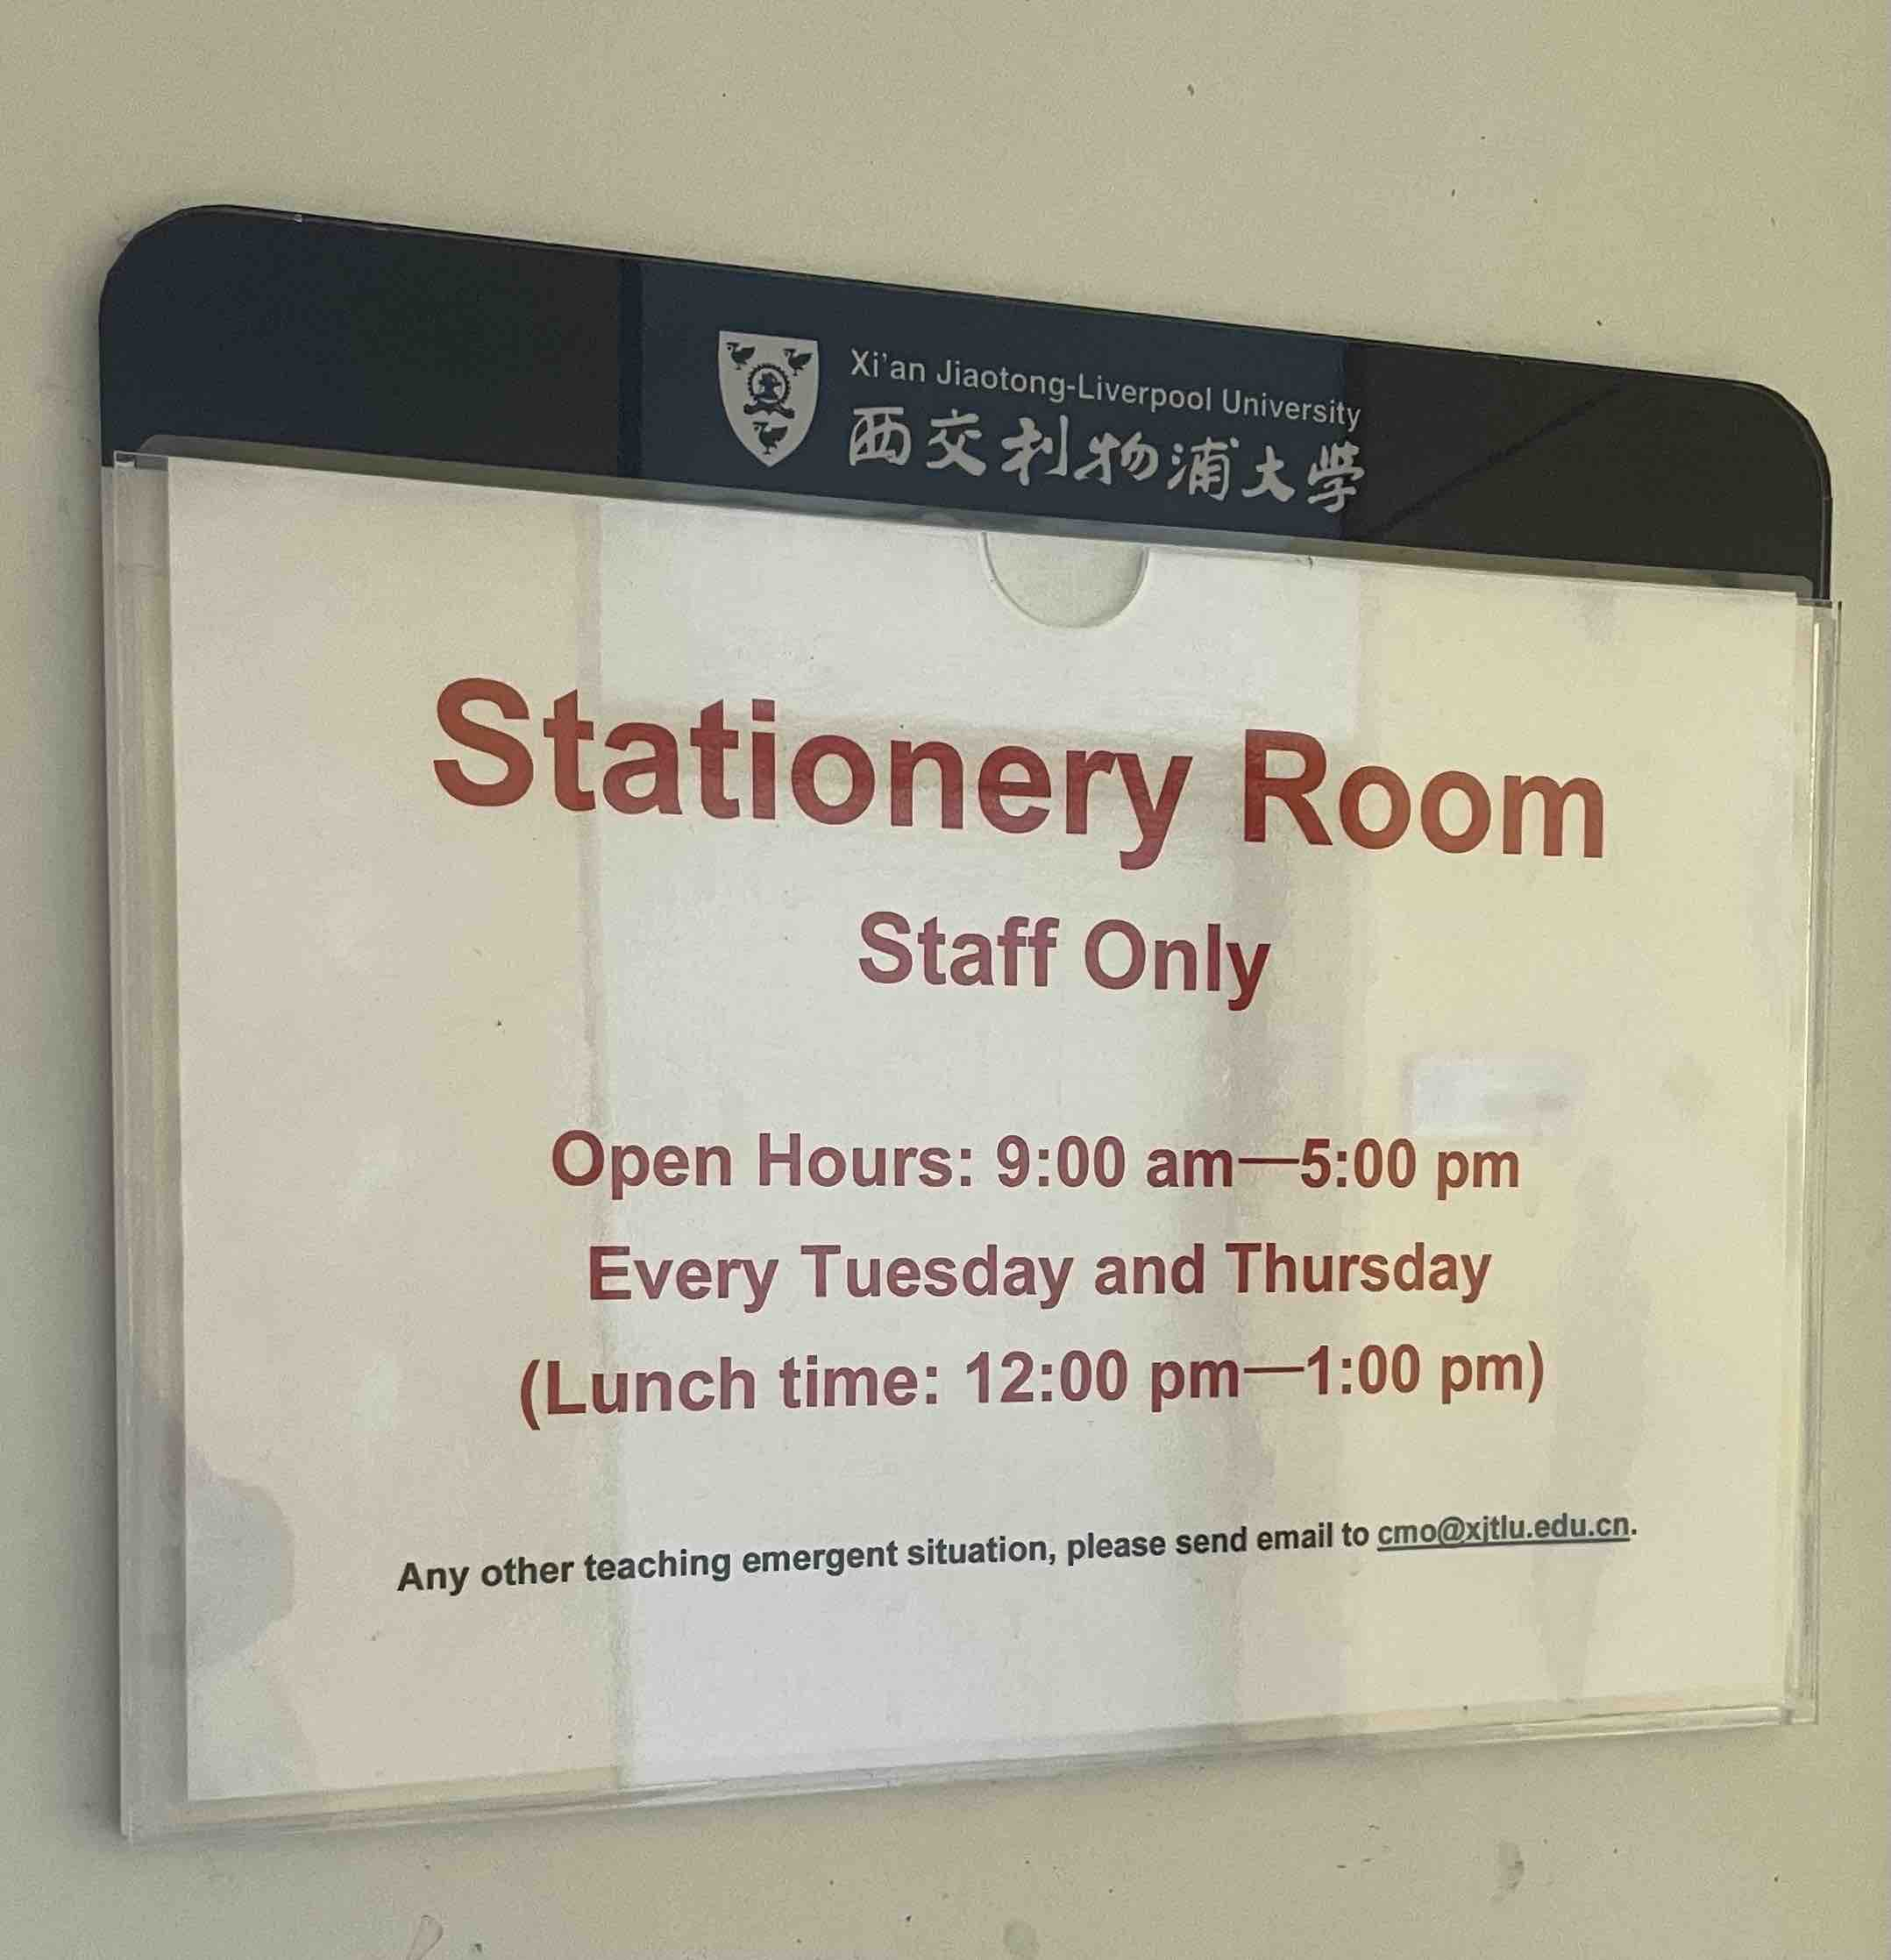
\includegraphics[width=0.6\columnwidth]{author-folder/Kai.Wu/stationery_room.jpg}
\end{figure}

Besides the substantial conference funds, the best way to save money is probably the free office supplies. Many buildings in the university have a Stationery Room (Office Supplies Collection Room), where all items are available for collection. Tissues, pens, markers, highlighters, various storage racks, tapes, glues, staplers—basically everything you can think of.

\vspace{5mm}
Locations of Stationery Rooms:
\begin{itemize}
    \item MB128, Tuesday/Thursday, 9–11 am, 1–5 pm
    \item BSG35, Tuesday/Thursday, 9–11 am, 1–5 pm (Thanks to an anonymous classmate for the addition)
    \item HS Building Property Office, Monday/Wednesday, 9–11 am, 1–5 pm, Friday morning (Thanks to an anonymous classmate for the addition)
    \item Other buildings? Please add
\end{itemize}

\hfill\break
How to collect:
\begin{enumerate}
    \item Before your first collection, go directly to the Stationery Room and ask the staff what items are available. They will give you a booklet. You can take photos of each page for reference, so you’ll know what you can get next time. Alternatively, you can find a historical version uploaded by a helpful classmate here \href{https://github.com/xp-pgrs-unofficial-guide/xp_pgrs_unofficial_guide/tree/main/fileshare}{[GitHub Link]} \href{https://gitee.com/kaiwu-astro/xp_pgrs_unofficial_guide/tree/main/fileshare}{[Alternate Link if you can't access GitHub]}, but the content may have slight differences due to changes.
    \item Download the latest (CMO) Office Supplies Application Form; the current latest version is V3. Old versions generally cannot be used after a new version is released. If this expires, where can we download the updated version? Unfortunately, we can't download it \sout{(complain about the university here)}; the usual method is to ask your supervisor, who can usually find it in the school's Box cloud storage. Here's the one I'm using \href{https://github.com/xp-pgrs-unofficial-guide/xp_pgrs_unofficial_guide/tree/main/fileshare}{Link} \href{https://gitee.com/kaiwu-astro/xp_pgrs_unofficial_guide/tree/main/fileshare}{Backup Link}.
    \item Fill in the form truthfully. The first column [Office Supplies Name] must exactly match the item names in the booklet mentioned above. You can't take too much at once; the staff will check. You can only take one box of tissues each time. Pens are generally taken individually, not by the box (but you can write down 12 pieces, which equals one box). For the reasons on the right, fill in truthfully and simply, such as Tissues—Daily Use; Pens—Calculations; Stapler—Organizing; Glue—Reimbursement. Finally, your supervisor needs to sign. Electronic signatures probably cannot be used, and you can't photocopy after your supervisor signs (these were common tricks in previous versions, haha). After filling it out, take it to the Stationery Room during open hours, and you can happily enjoy free shopping.
    \item Updated June 2023: The following items can be taken directly without filling out a form (others require the normal form)
\end{enumerate}

\begin{figure}[H]
    \centering
    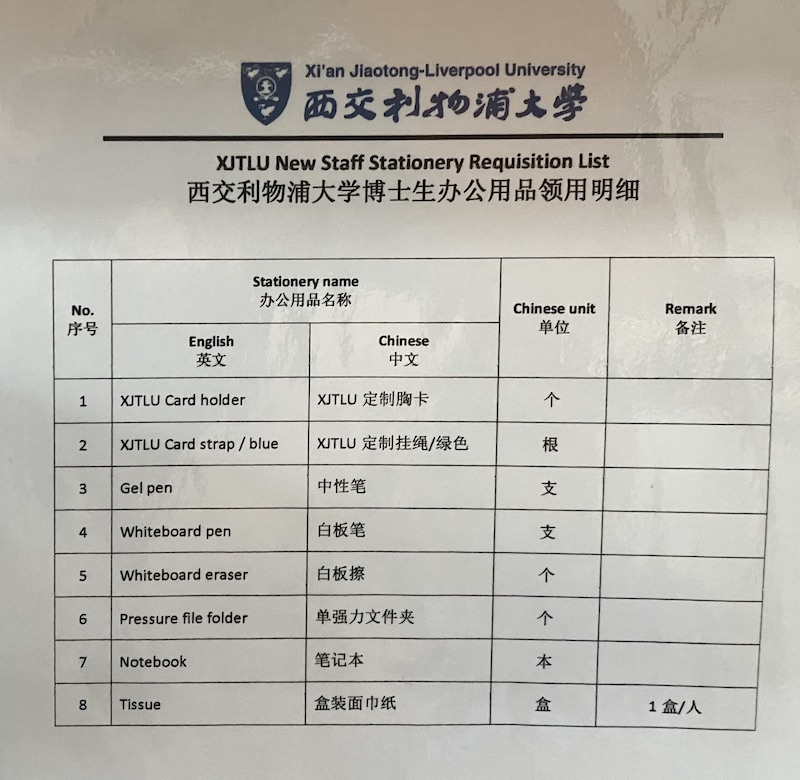
\includegraphics[width=0.6\columnwidth]{author-folder/Kai.Wu/stationery_no_sign.jpg}
\end{figure}

\begin{flushright}
    October 12, 2022 by \Wu \\
    GPT translation proofread by \Shiyao
\end{flushright}

\section{Free Printing}

Every September, the school resets the printing balance for PhD students to 2,000 yuan (you can check it at \url{https://myprint.xjtlu.edu.cn}), which means that each PhD student almost has unlimited printing funds. Personally, I like to print out all the papers to read.
For instructions on how to print, I suggest referring to the official documentation. The files are available in this project’s GitHub repository (link below) or at the following links:
Undergraduate IT Guide (in Chinese and English): \url{https://gitee.com/kaiwu-astro/xp_pgrs_unofficial_guide/tree/main/fileshare}
Printing Guide (in English): \url{https://guide.xjtlu.edu.cn/ss-print/staff}
Please note, do not use this for printing entire books as it violates the printing policy and may be detected. However, printing individual chapters of books is generally allowed. If you must print an entire book, please use Taobao.

\begin{flushright} 
    October 12, 2022 by \Wu \\
    GPT translation proofread by \Shiyao
\end{flushright}
\section{Gym Vouchers}
\begin{minipage}[t]{0.5\textwidth}
    The school gym operates commercially, which means it charges fees. However, the WeChat mini-program “XJTLU Sports Center” distributes vouchers worth 100 yuan every month. These can be used for booking basketball courts, table tennis tables, gym time, etc. For more details, please explore the mini-program. In fact, the school’s gym facilities are very comprehensive and quite new. If you haven’t been there yet, go explore it soon. The vouchers are essentially [expiring balance], which means they will automatically adjust. For example, if you book a gym session for 25 yuan using a 100 yuan voucher, the voucher balance will become 75 yuan, but the vouchers do have an expiration date.

    After booking, you need to swipe your XJTLU campus card to enter the gym’s main entrance, and then scan the QR code of the booked facility to enter the specific venue.

    \begin{flushright}
    (October 12, 2022 by \Wu) \\
    (Translated by GPT)
    \end{flushright}
\end{minipage}
\begin{minipage}[t]{0.45\textwidth}
    \begin{figure}[H]
        
\includegraphics[width=0.95\columnwidth, right]{author-folder/Kai.Wu/sportcenter_miniprogram.jpg}
    \end{figure}
\end{minipage}

\section{Benefits come with UoL Account}
\label{sec.fuli_liverpool}
\begin{itemize}
    \item Zoom Premium account: \url{https://liverpool.service-now.com/sp?id=kb_article&sysparm_article=KB0011854}
    \item Office 365: \url{https://liverpool.service-now.com/sp?id=kb_article&sysparm_article=KB0010032}
    \item 1 TB Onedrive cloud storage:  \url{https://liverpool.service-now.com/sp?id=kb_article&sysparm_article=KB0011362}
    \item 1 TB Onedrive cloud storage local synchronization: \url{https://support.microsoft.com/zh-cn/office/%E4%BD%BF%E7%94%A8-onedrive-%E8%BF%9B%E8%A1%8C%E5%90%8C%E6%AD%A5-bb89981b-e382-4969-b8fd-d413a90b6db3}
    \item Other free softwares: \url{https://www.liverpool.ac.uk/it/software/software-downloads/}
    \item Software license: \url{https://www.liverpool.ac.uk/it/software/licencecodes/}
\end{itemize}

\begin{flushright}
    (October 2, 2022 by \Wu) \\
    (Translated by \Shiyao)
    \end{flushright}
% Rumor has it that PhD students no longer receive student IDs, so the guide below is obsolete
% \section{景区学生票(和火车票学生票)优惠}

% 传闻最新情况博士生不发学生证,本篇攻略废弃

和本科生一样,我们也是能享受学生票优惠的。步骤如下

\begin{enumerate}
    \item 申请学生证。学生证,不是你的ID卡,是红色的小本本。博士生,默认是不发学生证的,要自己申请才发。方法:在一站式网站 \url{https://studentonestop.xjtlu.edu.cn/} 里的申请/补办学生证,按提示操作。学生证可用于各景点买学生票(例如拙政园,买学生票过后进门查学生证。ID卡是不行的)。
    \item 据部分同学反应,一站式老师说给我们的学生证是给本科生发完后剩下的,如果不剩了就只能等新一批。我不知道不发学生证是否合规,具体可骚扰一站式或pgsupport。
    \item 据部分同学反应,2020年之后给博士生发的学生证没有火车票优惠卡了(最后一页上的芯片小贴纸),我不知道不发这个是否合规,具体可骚扰一站式或pgsupport。如果你的学生证没有火车票优惠卡,就不能买火车票的学生票,但景区优惠不受影响。
    \item 注意盖注册章:在景区门口(或火车上)如果遇到工作人员double check你学生身份,发现你学生证注册章不是最新的,按政策是可以要求你补全票的。所以,去景区(或坐火车)之前,要注意注册章要盖够了。我的做法是,买学生票的时候再去check自己注册章有没有盖够,否则立马去一站式补就行(可以一口气盖一堆)。
    \item 
        \begin{minipage}{0.71\textwidth}
            如果你有火车票优惠卡,可以继续看这部分:如何使用?如何购买火车票学生票?有什么限制?因为政策可能变动,请直接关注官方公众号,在公众号菜单里有常见问题FAQ。
        \end{minipage}
        \begin{minipage}{0.2\textwidth}
            \begin{figure}[H]
                
\includegraphics[width=0.95\columnwidth, center]{author-folder/Kai.Wu/qrcode_huitongstudent_1.jpg}
            \end{figure}
        \end{minipage}

\end{enumerate}


\begin{flushright}
(2023年01月04日 by \Wu)
\end{flushright}

% \begin{figure}[H]
%     \centering
%     \includegraphics[width=0.5\columnwidth]{author-folder/Kai.Wu/}
% \end{figure}


% \usepackage[export]{adjustbox}

% \item 

% \begin{newminipage}[0.65]
%     文字
% \end{newminipage}
% \begin{newminipage}[0.34]
%     \begin{figure}[H]
%         % \caption{}
%         \includegraphics[width=0.95\columnwidth, right]{author-folder/Kai.Wu/}
%     \end{figure}
% \end{newminipage}

% \input{author-folder/Kai.Wu/.tex}


\section{Other Benefits}

If you haven't seen the content below, you can spend a few minutes exploring it. Leaving an impression may be very helpful in the future.

\begin{enumerate}
    \item IT services provided by the university: \url{https://guide.xjtlu.edu.cn/it-guide-for-student.html}, including free Office 365
    \item (Readers are welcome to contribute)
\end{enumerate}

\begin{flushright}
    Translated by GPT
\end{flushright}
% %# -*- coding: utf-8-unix -*-

\chapter{最好要知道这些}

\section{How does Research Work}
\label{section.how-research-works}

\subsection{Funding}
Academic funding generally comes from the following three sources:
\begin{itemize}
    \item Government Agencies and Foundations: In China, there are grants available from the central government, provinces, and cities, aimed at both projects and individuals. Similarly, abroad, there are government-supported societies that provide grants. These projects usually have large amounts of funding and high impact. A successful application record in this system can significantly help in applying for similar projects in the future.
    \item Corporate Collaboration Projects: These are typically obtained by project leaders through negotiations with companies, and most of these projects focus on practical implementation. The amount of funding, completion rate, and impact can vary widely.
    \item Internal Research Support Projects (such as RDF): These are applied for by faculty members within the school, screened by the college, and reviewed by a specific committee. The number of projects is limited, the funding amounts are small, and the duration is short, but they are important for early-career researchers.
\end{itemize}

Academic funds do not go directly into the project leader’s personal bank account but into the school’s research fund management account. Expenditures must comply with specified spending categories and are subject to school regulations, commonly including procurement, conference-related expenses, labor costs, etc.

When academic funding exceeds a certain amount, the advisor can obtain corresponding PostGraduate Research student Scholarship (PGRS) slots based on the amount of funding.


\subsection{Journals and Conferences}
Journals and conferences require at least one academic organization to host the event. Important and active researchers often take on roles such as editors and reviewers within these organizations, which helps attract submissions and participation. Correspondingly, taking on roles in academic organizations reflects a researcher’s reputation to some extent.

Publishers need financial support to publish journals and host conferences. Generally, the more important, influential, and valuable a journal or conference is, the easier it is to find sponsors, the less authors need to pay for publication fees, and the higher the scale, richness, and quality of the event.

The impact of journals and conferences is largely influenced by the citation count of published articles. More trendy topics, significant work, well-known authors, and important journals are more likely to be read and cited. To ensure sustainability, organizers also prioritize these factors.

In many research fields, the number of researchers is small, so attending conferences often means meeting people who have at least read your papers, and possibly even reviewers or viva examiners.


\subsection{Social Benefits}
One aspect of academic research is creating new knowledge at the limits of human cognition. From this perspective, academic research will ultimately benefit society.

Additionally, it is said that the humanities and social sciences also like to focus on social impact. We might invite someone to write about this in the future.

However, considering we live in a commercial society, social benefits often equate to the monetary value or potential of the results. This is also the environment we find ourselves in physically.


\subsection{Supervisors}
Different supervisors have different characteristics, but they can roughly be divided into application-oriented and frontier-oriented:
\begin{itemize}
    \item Application-Oriented supervisors: These advisors generally have more practical projects from enterprises or government, or application-oriented grants from the government.
    \item Frontier-Oriented supervisors: These advisors usually have more significant work published.
\end{itemize}

\vspace{\baselineskip}

These are not mutually exclusive; it’s just that time and energy are limited, so there will always be a certain inclination. Relatively speaking, there are more opportunities in application-oriented projects, while frontier-oriented projects require larger funding amounts. Due to the different inclinations of advisors, the resources they develop also differ, and the guidance you receive will vary.

Based on the above reasons, you might agree that we are likely to become like our advisors.

For the humanities and social sciences, it is said that almost full-time mentorship is required. We might invite someone to write about this in the future.

\subsection{Teamwork}
\label{subsection.teamwork}
When conducting academic research, we may inevitably collaborate with other researchers for various reasons, including:
\begin{itemize}
    \item Research Funding: Well, since they provide the funding, it makes sense for them to give some input and be listed as authors. \dots
    \item Academic Influence: Interestingly, experience suggests that articles involving prominent researchers are more likely to be accepted. \dots
    \item Private Data: In many fields, data privacy is an unavoidable norm. \dots
    \item Expertise: Many studies are interdisciplinary, and you might not understand all the details. Finding a researcher familiar with a particular aspect of the work can be very helpful, saving you a lot of effort and improving research efficiency. Of course, choosing the right person requires careful consideration. \dots
    \item Experimental Work: Similar to expertise, suitable collaborators can save you a lot of effort. It is also common to hear about people enlisting undergraduates to help with experiments and co-authoring publications. \dots
\end{itemize}

\vspace{\baselineskip}

Additionally, before you start collaborating with researchers outside your advisor’s team, be sure to read the school’s \href{https://ebridge.xjtlu.edu.cn/urd/sits.urd/run/SIW_FILE_LOAD.start_url?08F2CBCAE3174A7365Px9_5kBfG0_iGiWj8zb7ybwaO0YBYc8NiKlPG93xyQA9X2SClXOLLd7-_EgF50aijROwT-rdSGIUIbRRzhFu-76Ha0g2HymUr0S-Fgjm1DXP9RO1GhGzx5-akgsDSMBlNhR7vpib85F9vlqa67My7RKHFSiluZueFy52YCBtintt0wDTKmx4fCjkWnldNDaxo6ZVD2L572Us3V-FOv485wYZUNUn5NLzgR0pAaU7aiKnTVJY8Aa2su5F4u7o-rNPJPety3jwwJ4O1v1agpDZLZ1it1H5fWn3IgLNaWlUh84YpxNRXyTW1kIwrX0r4-dT1eoxdZUAFrJhaBwz6E0w}{Guidance on Authorship and Affiliation}, which might save you a lot of trouble.

\begin{flushright}
    2024年10月1日 by \Shiyao \\
    Translated by GPT
\end{flushright} \clearpage

\section{Teaching Assistant}

\subsection{Do I have to be a TA?}
\begin{itemize}
    \item If you are a full scholarship PhD student (tuition waiver + stipend), according to the Financial Offer from the school, you have TA obligations every semester (in other words, the scholarship is in exchange for TA work; you must work if you receive the money). After working as a TA, you will not receive additional wages. For full scholarship PhD students enrolled in 2020 and later, they must complete 900 hours of TA work over three years to graduate. For those enrolled in 2023 and later, they must complete 300-500 hours of TA or RA work each academic year to graduate.
    \item If you are a half-scholarship PhD student (tuition waiver only) or a self-funded student enrolled in 2020 and later, you have no obligation to work as a TA. After working as a TA, the school will pay you according to the hours worked, and the TA experience can be added to your resume, which might be beneficial depending on your future career plans.
\end{itemize}

For full scholarship students, the mandatory 300 hours of TA work per academic year equates to approximately 7.5 hours of duty per week over 40 teaching weeks, roughly equivalent to one day per week. You might wonder if this is strictly enforced. In practice, enforcement varies significantly between colleges. Some colleges have established a digital system to track your hours, requiring you to meet the quota, while others are more lenient. For specific enforcement details, please consult senior students in your program.

\begin{flushright}
    (2022年10月21日 by \Wu)

    (major update: December 30, 2022 by Yue Zhou: Updated TA hours according to the latest official handbook)

    (update: January 15, 2024 by \Wu : Updated TA hours according to the latest official handbook)

    (Translated by GPT)
\end{flushright}

\subsection{How to Become a TA}

Around the first week of each semester, the college will recruit TAs, usually through the School Academic Administrator.
\begin{itemize}
    \item Half-scholarship and self-funded PhD students have more freedom and can contact the course instructors directly.
    \item Full scholarship PhD students have two scenarios: a) contacting course instructors directly, or b) being assigned by the college via email.
\end{itemize}

If you are eager to participate or want to secure a spot in a particular course or with a specific instructor, contact the administrator and the relevant course instructor as early as possible.

\begin{flushright}
    (December 30, 2022 by Yue Zhou) \\
    (Translated by GPT)
\end{flushright}

\subsection{Types of TA Work and How to Do Them}

TA duties include but are not limited to:
\begin{enumerate}
    \item Grading assignments and exams
    \item Conducting tutorials (mostly in business courses) and labs
    \item Calculating and recording course grades
    \item Performing auxiliary tasks (e.g., setting up Learning Mall)
    \item Proctoring midterm and final exams
\end{enumerate}

The Graduate School organizes TA training sessions, which are announced via emails titled \textit{Teaching Assistant (TA) Training Programme} and can also be found on your Learning Mall. These sessions are held every semester. If you have never attended any, it is recommended to attend at least once. Below are some core contents that the school’s training might not cover in detail:

\subsubsection{Grading Assignments}
If grading traditional paper-based assignments, generally ask the instructor how to proceed. For electronic assignments submitted through the Learning Mall (referred to as LMO), here is a tutorial:
\begin{enumerate}
    \item Log in to LMO and find the course you are assisting. If you cannot find it, email your school administrator or the course instructor to grant you access.
    \begin{figure}[H]
        \centering
        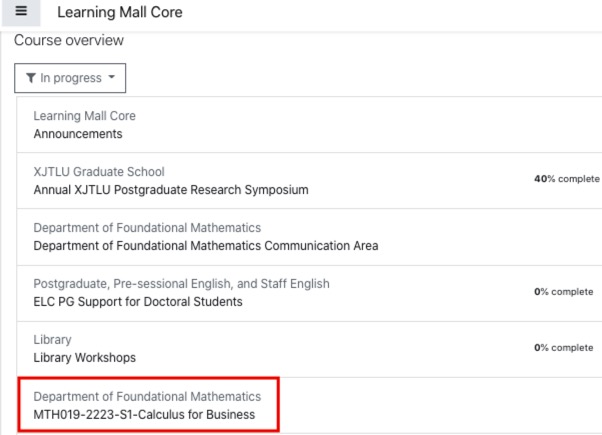
\includegraphics[width=0.4\columnwidth]{author-folder/Kai.Wu/LMO_course.jpg}
    \end{figure}

    \item 
    \begin{minipage}{0.3\textwidth}
        Enter the course, scroll down to find the submission area, or use Ctrl+F (Command+F on Mac) to search for “submission”.
    \end{minipage}
    \begin{minipage}{0.63\textwidth}
        \begin{figure}[H]
            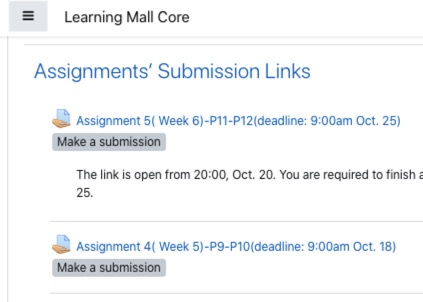
\includegraphics[width=0.95\columnwidth, right]{author-folder/Kai.Wu/LMO_submission_links.jpg}
        \end{figure}
    \end{minipage}

    \item For large required courses with many sections, first select the group you are assigned to grade. Next, if you want to start grading online immediately, click “Grade.” If you want to review or grade offline (e.g., download to an iPad), click “View all submissions.”
        \begin{figure}[H]
            \centering
            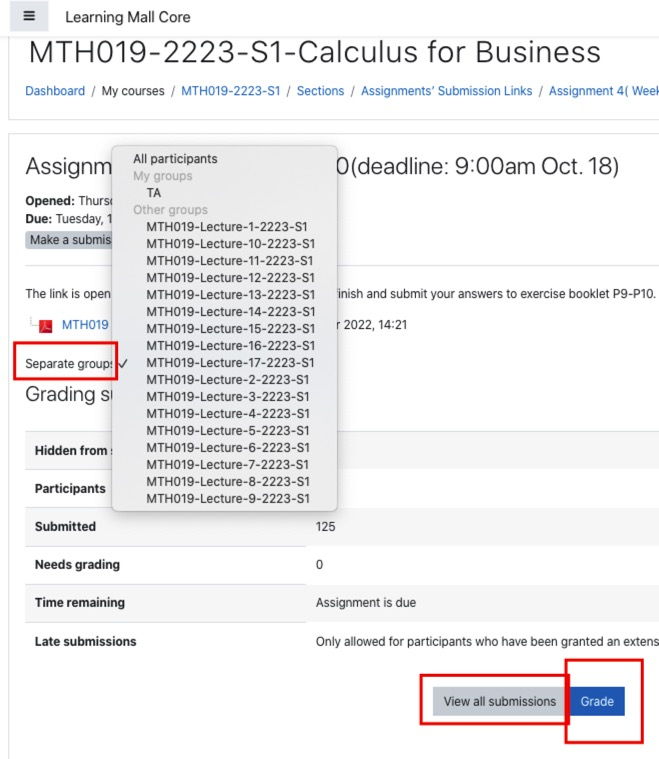
\includegraphics[width=0.5\columnwidth]{author-folder/Kai.Wu/LMO_inside_submission.jpg}
        \end{figure}
    \item The online grading system can be very slow and the PDF annotation tools are cumbersome, making online grading inefficient unless the instructor has provided a grading rubric (my advisor showed me once where you can select scores and reasons for each part of the assignment directly on the right side). Otherwise, online grading is not very useful. Below is a relatively efficient offline grading method I have figured out. After clicking “View all submissions,” select “Download grading worksheet” and “Download all submissions” from the “Grading action” menu.
        \begin{figure}[H]
            \centering
            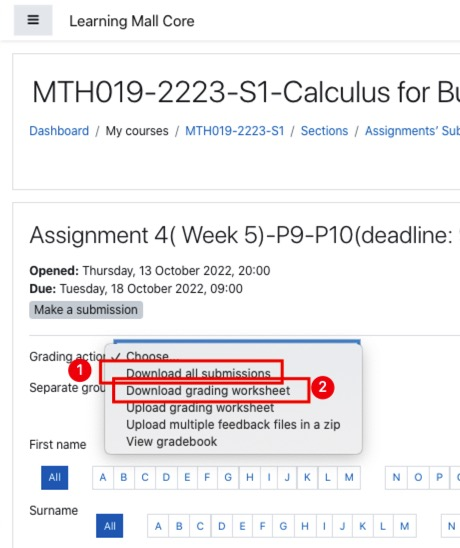
\includegraphics[width=0.5\columnwidth]{author-folder/Kai.Wu/LMO_download.jpg}
        \end{figure}
    \item You will receive a CSV file and a large ZIP file. Extract the ZIP to see all the student submissions named by student name and ID. You can then grade these files locally on your computer or tablet. If your instructor does not require the graded assignments to be returned as feedback files (ask your instructor), you can even print them out to grade. After grading, record the grades in the grading worksheet. The CSV can be opened with Excel, and you can save it as an XLSX file. The last column of the spreadsheet is “Feedback comments,” where you can write comments for students, such as “incorrect file format” or “please submit clearer images next time.”
        \begin{figure}[H]
            \centering
            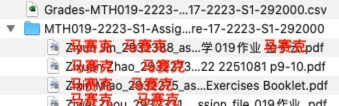
\includegraphics[width=0.5\columnwidth]{author-folder/Kai.Wu/LMO_Downloaded.jpg}
        \end{figure}
    \item After grading according to the instructor’s requirements, you can easily upload the grading worksheet and graded files (if required) back to LMO. From the “View all submissions” page, click “Upload grading worksheet” to upload the grading worksheet.
        \begin{figure}[H]
            \centering
            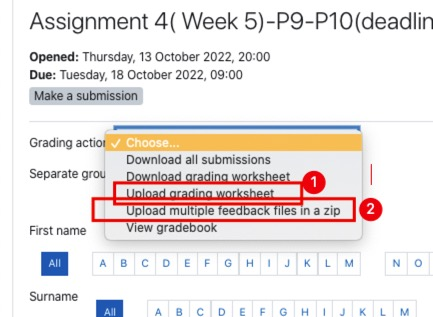
\includegraphics[width=0.5\columnwidth]{author-folder/Kai.Wu/LMO_upload.jpg}
        \end{figure}
    \item If you saved the worksheet as an XLSX file, save it as a UTF-8 CSV file before uploading. Check the “Allow this CSV to override existing grades” box. After clicking “Upload,” you will see a long webpage with each student’s grade and your feedback comments uploaded. 
        \begin{figure}[H]
            \centering
            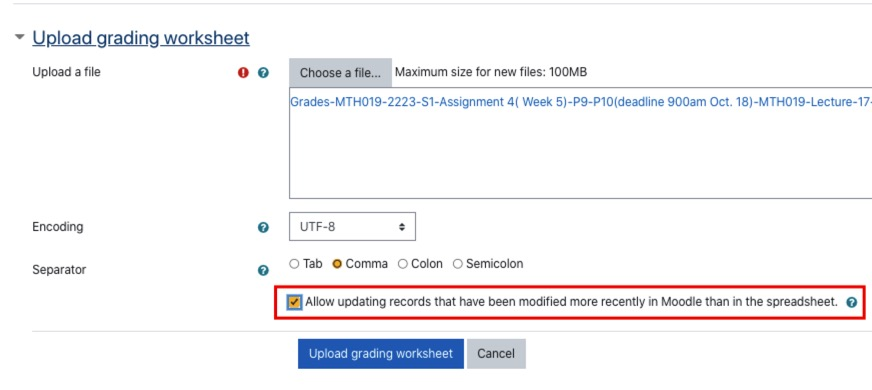
\includegraphics[width=0.8\columnwidth]{author-folder/Kai.Wu/LMO_upload_sheet.jpg}
        \end{figure}
    \item From the same page, click “Upload multiple feedback files in a ZIP” to upload the graded assignments. Zip the graded files, but if the total size exceeds 100MB, you will need to manually split them into multiple ZIP files smaller than 100MB (annoying, but LMO restricts uploads to 100MB). If you know Python, you can use my script \href{https://github.com/kaiwu-astro/xp_pgrs_unofficial_guide/tree/main/fileshare/zip_in_100M.py}{GitHub repo} or \href{https://gitee.com/kaiwu-astro/xp_pgrs_unofficial_guide/tree/main/fileshare}{Gitee repo} to automatically split the files into 100MB ZIPs. After uploading, you are done.
    \item Finally, email the instructor to report (1) common issues, such as frequently missed questions or common misunderstandings, (2) individual issues, such as students submitting the wrong files, suspected plagiarism, or similar assignments, and (3) any other issues you want to discuss with the instructor. The math department has a feedback form for this purpose. If there is no feedback form, you can email the instructor. (Generally, you don’t need to be too detailed unless you are passionate about this work, as it can be time-consuming.) 
        \begin{figure}[H]
            \centering
            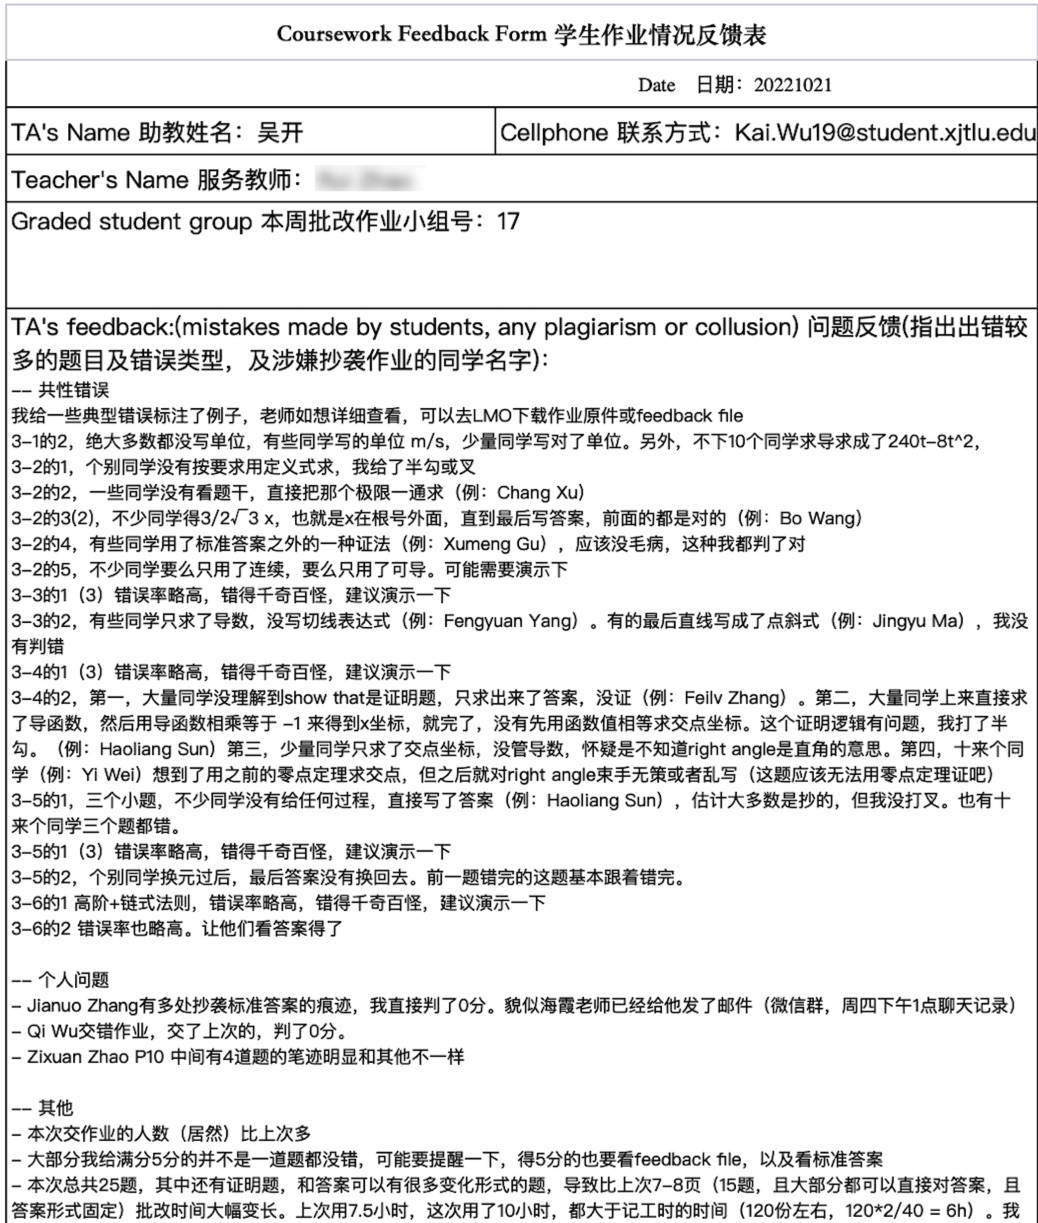
\includegraphics[width=0.5\columnwidth]{author-folder/Kai.Wu/LMO_feedback_to_teacher.jpg}
        \end{figure}
\end{enumerate}


\emptyline
Tips for Grading Assignments
\begin{enumerate}
    \item My tool combination is an iPad + Apple Pencil + PDF Expert app, which is much faster than grading online or offline on a computer. Additionally, purchasing a magnetic paper-like screen protector (about 20 yuan) and replacement pencil tips (about 10 yuan) can significantly improve the writing experience.
        \begin{figure}[H]
            \centering
            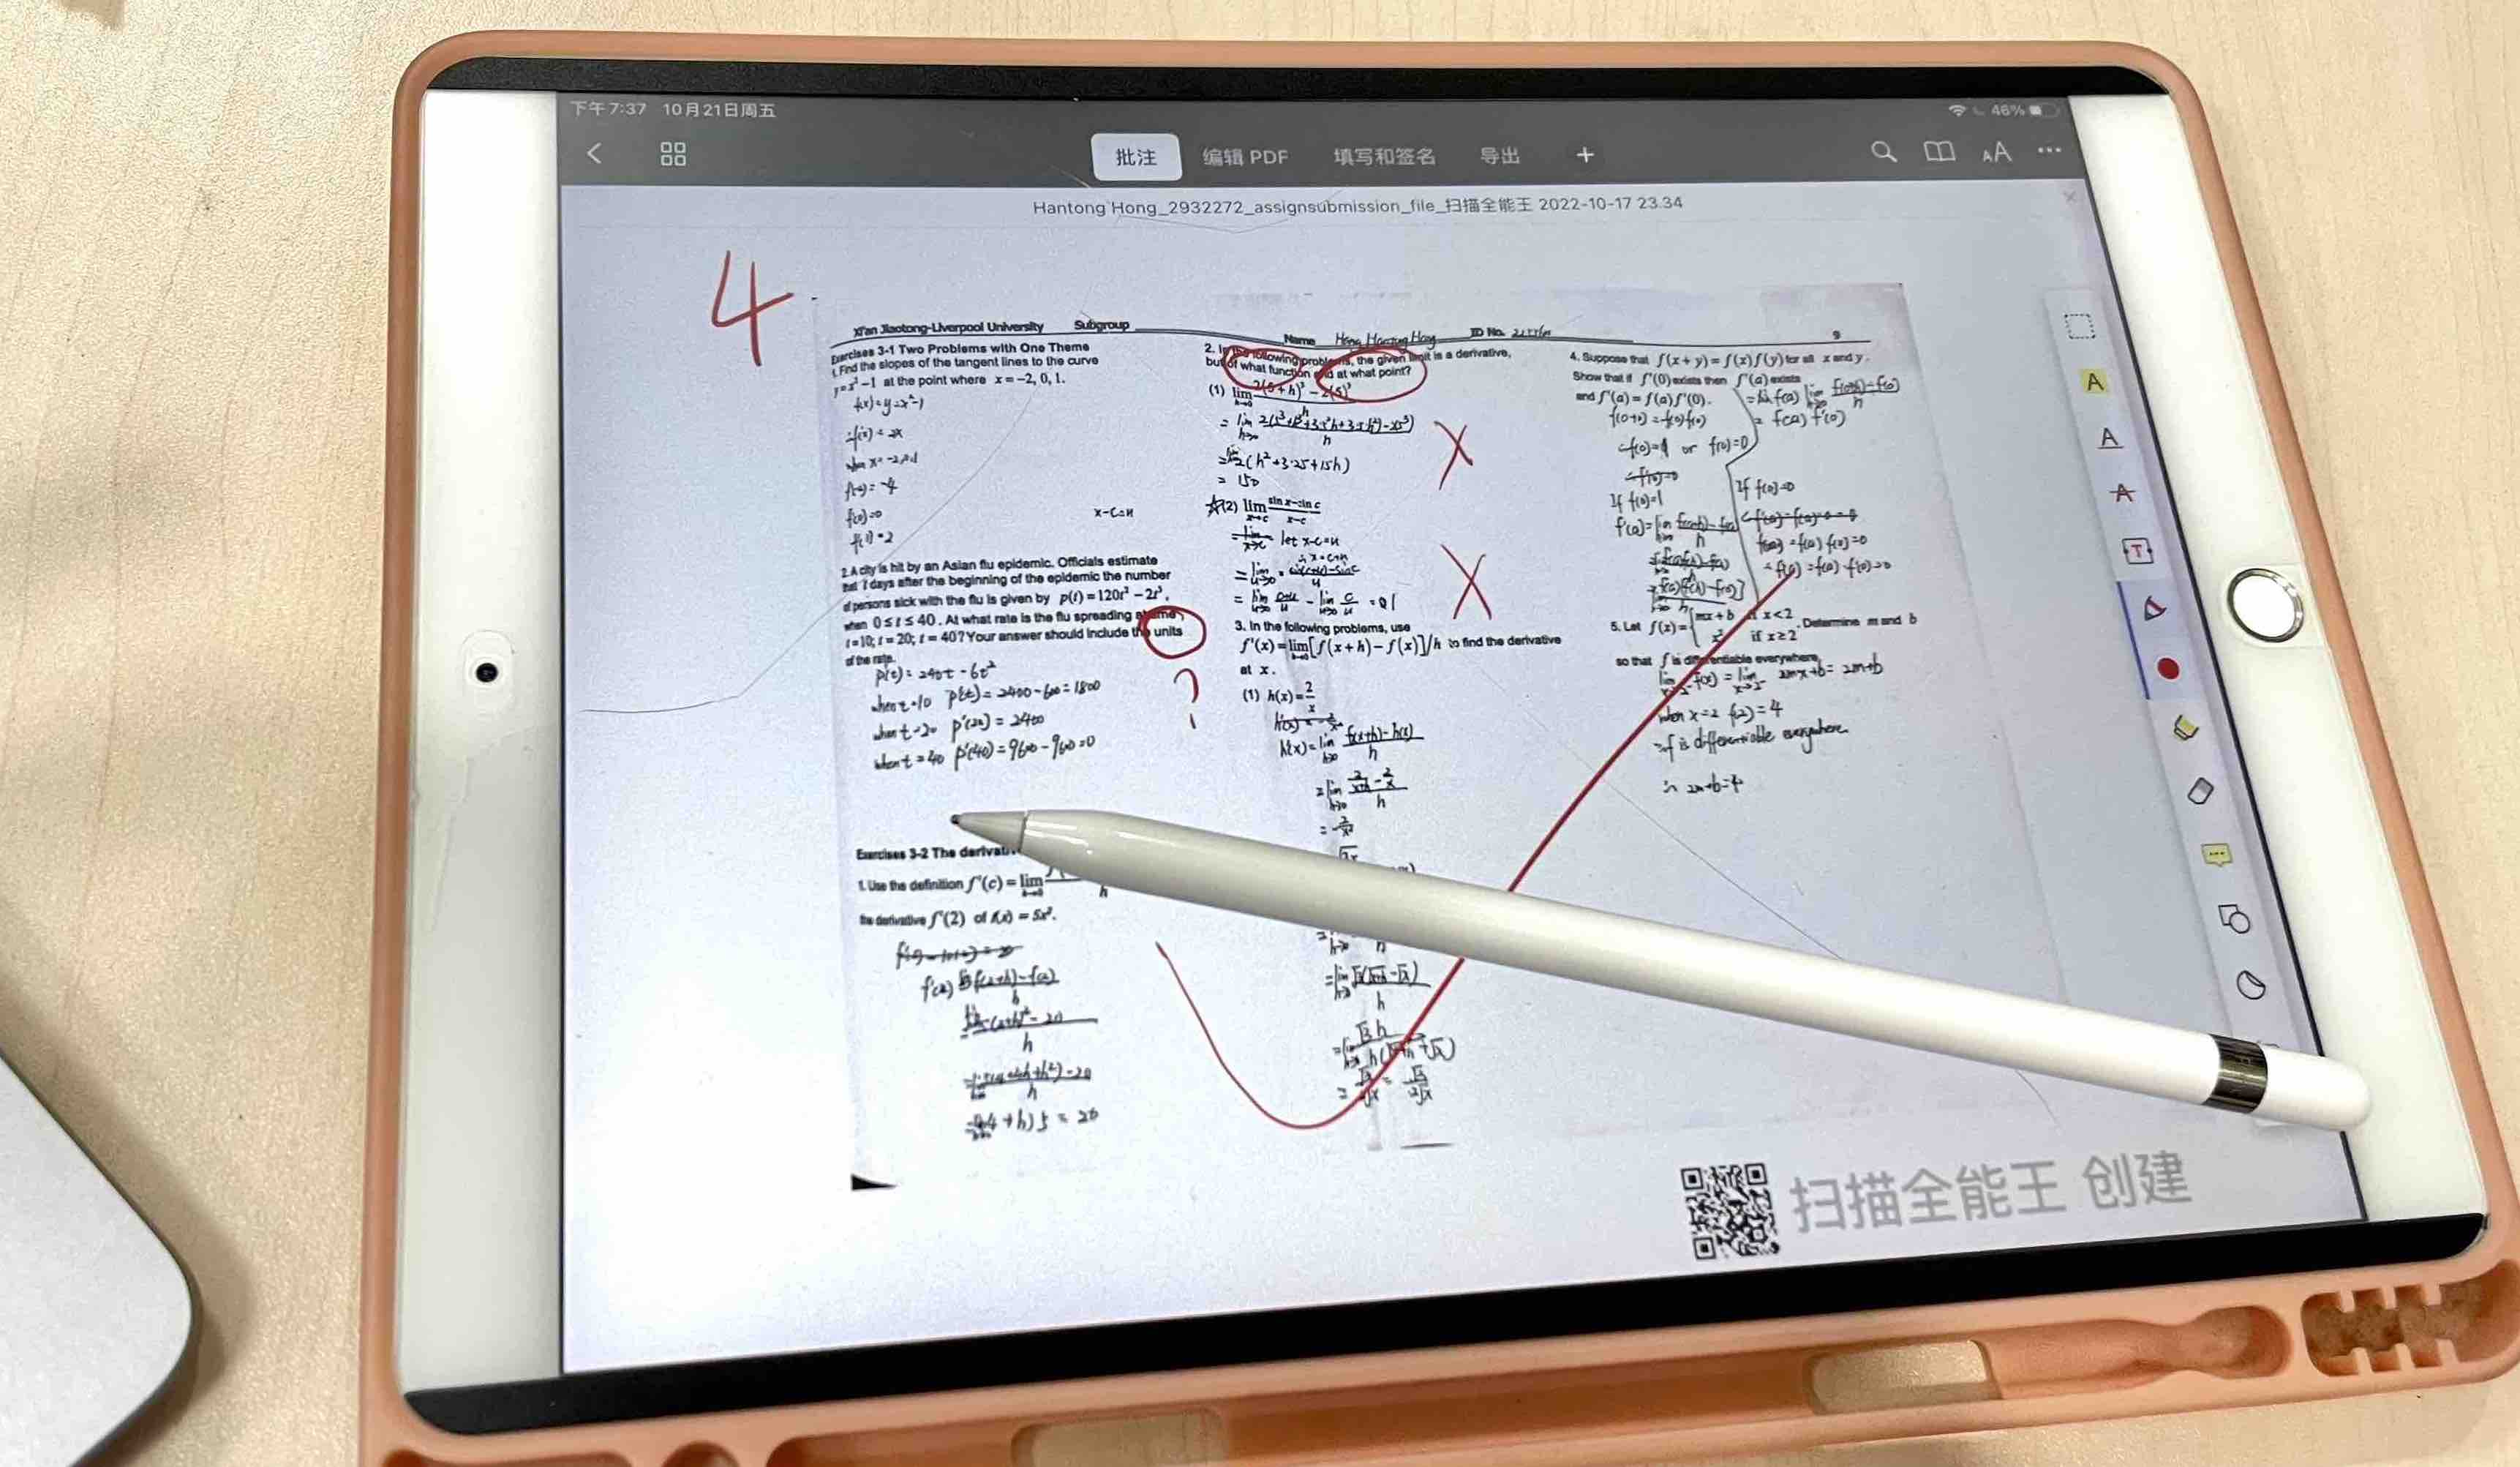
\includegraphics[width=0.5\columnwidth]{author-folder/Kai.Wu/marking_tools.jpg}
        \end{figure}
    \item Improve efficiency with an assembly line approach: When there are many questions, don’t grade all parts of one student’s assignment before moving to the next. Instead, grade all assignments’ part 1 (e.g., the first three questions), then go back and grade all part 2 (e.g., questions 4-6).
    \item Although opening and closing files takes time, this method helps you remember the answers and grading points, speeding up the process. Avoid looking at the answers for each assignment.
Similarly, don’t record grades one by one. My habit is to write the total score in large numbers in the top left corner. After grading all assignments, use the largest thumbnail view (Mac: View as Icons, press Command+Equal repeatedly; Windows: View as Extra Large Icons) to see the scores without opening the files. Sort by name in both Excel and the folder to quickly record the grades.
        \begin{figure}[H]
            \centering
            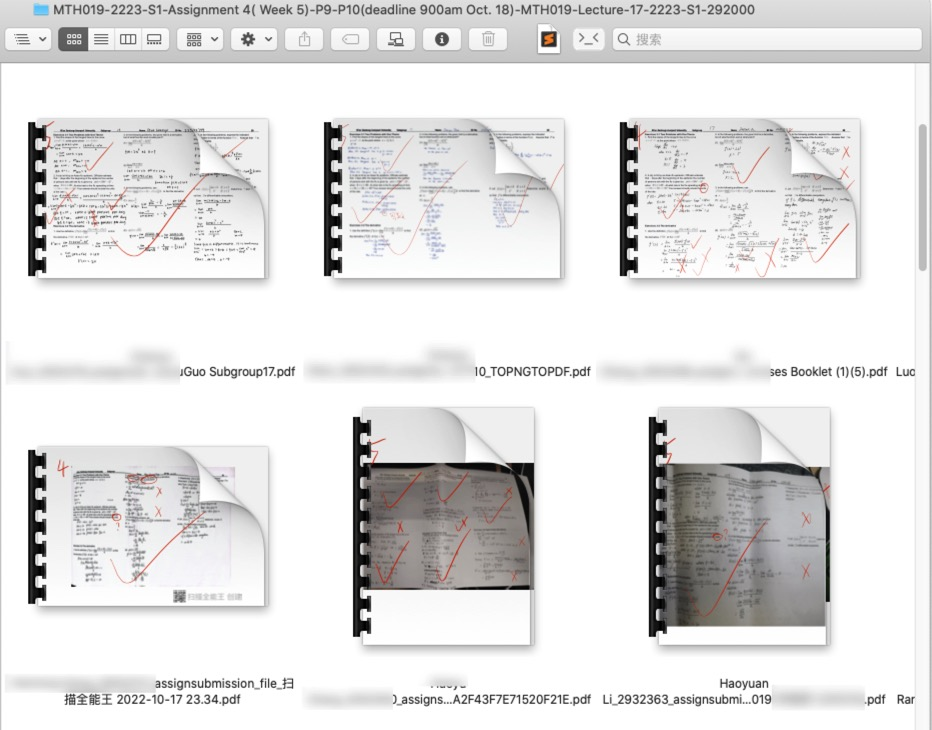
\includegraphics[width=0.7\columnwidth]{author-folder/Kai.Wu/tongchengji.jpg}
        \end{figure}
    \item Students may submit files with various issues, such as submitting Word or PPT instead of PDF, submitting PDFs with images in the wrong order or orientation, or writing on notebooks instead of using standard templates. TAs have the right to require students to follow specific formats and can warn students in the feedback comments. Remind the course instructor to emphasize this in class. If students continue to submit incorrect formats, you can deduct points according to your standards (e.g., first warning, second time deduct 20\%, third time deduct 50\%, fourth time deduct all).
    \item Sometimes, large files or files with many handwritten notes cause PDFs to open slowly or crash. For large files, ask students to compress the PDFs. For handwritten notes, there is no good solution. I wrote a Python script \href{https://github.com/kaiwu-astro/xp_pgrs_unofficial_guide/tree/main/fileshare/pdf_to_png_to_pdf.py}{[GitHub Link]}to convert PDFs to images and back to PDFs, making them open faster and reducing file size to under 5MB. Use it if needed, but it’s a bit complicated. I couldn’t find a better method.
    \item (Quietly) When unsure about the score, give a bit more. If you give too little, students will argue, wasting time. Giving a bit more saves your time.
    \item When recording grades, mistakes are inevitable, especially for new TAs. Consider double-checking everything. Writing the grade on the top left of the PDF helps, as students can see discrepancies between LMO and PDF grades and contact you.
    \item After grading, students may message you through LMO or email. Avoid replying directly to students, as mistakes can cause issues for the instructor. Forward all student messages to the instructor and let them reply unless they allow you to respond directly.
\end{enumerate}

\begin{flushright}
    (October 21, 2022 by \Wu) \\
    (Translated by GPT)
\end{flushright}

\subsubsection{Grading Exams}
For quizzes, midterms, and final exams, TAs may need to participate in grading. Before leaving for vacation at the end of the semester, confirm with the instructor to avoid missing grading responsibilities. If you need to leave early, discuss it with the instructor.

\subsubsection{Conducting Labs}
\begin{minipage}[t]{0.55\textwidth}
    For courses like university physics labs, TAs may need to conduct lab sessions. The typical process involves explaining the experiment principles, data recording and processing, and precautions on the lab whiteboard, followed by a hands-on demonstration. After the class, TAs need to grade lab reports.

    I find lab sessions very challenging because they involve real teaching in a university setting. You need to prepare lessons, organize your thoughts, and anticipate students' questions. The course instructor will train TAs in the lab, and you must understand the experiments thoroughly. Handling emergencies, such as students damaging equipment, requires immediate consultation with the instructor. Although lab sessions are few and the total work hours, including grading lab reports, are less than grading assignments for most other courses, they are very rewarding. If you want to challenge yourself, give it a try. If not, request a transfer to another course with the instructor and the school administrator early on.
    \begin{flushright}
        (October 22, 2022 by \Wu) \\
        (Translated by GPT)
    \end{flushright}
\end{minipage}
%
\begin{minipage}[t]{0.45\textwidth}
    \begin{figure}[H]
        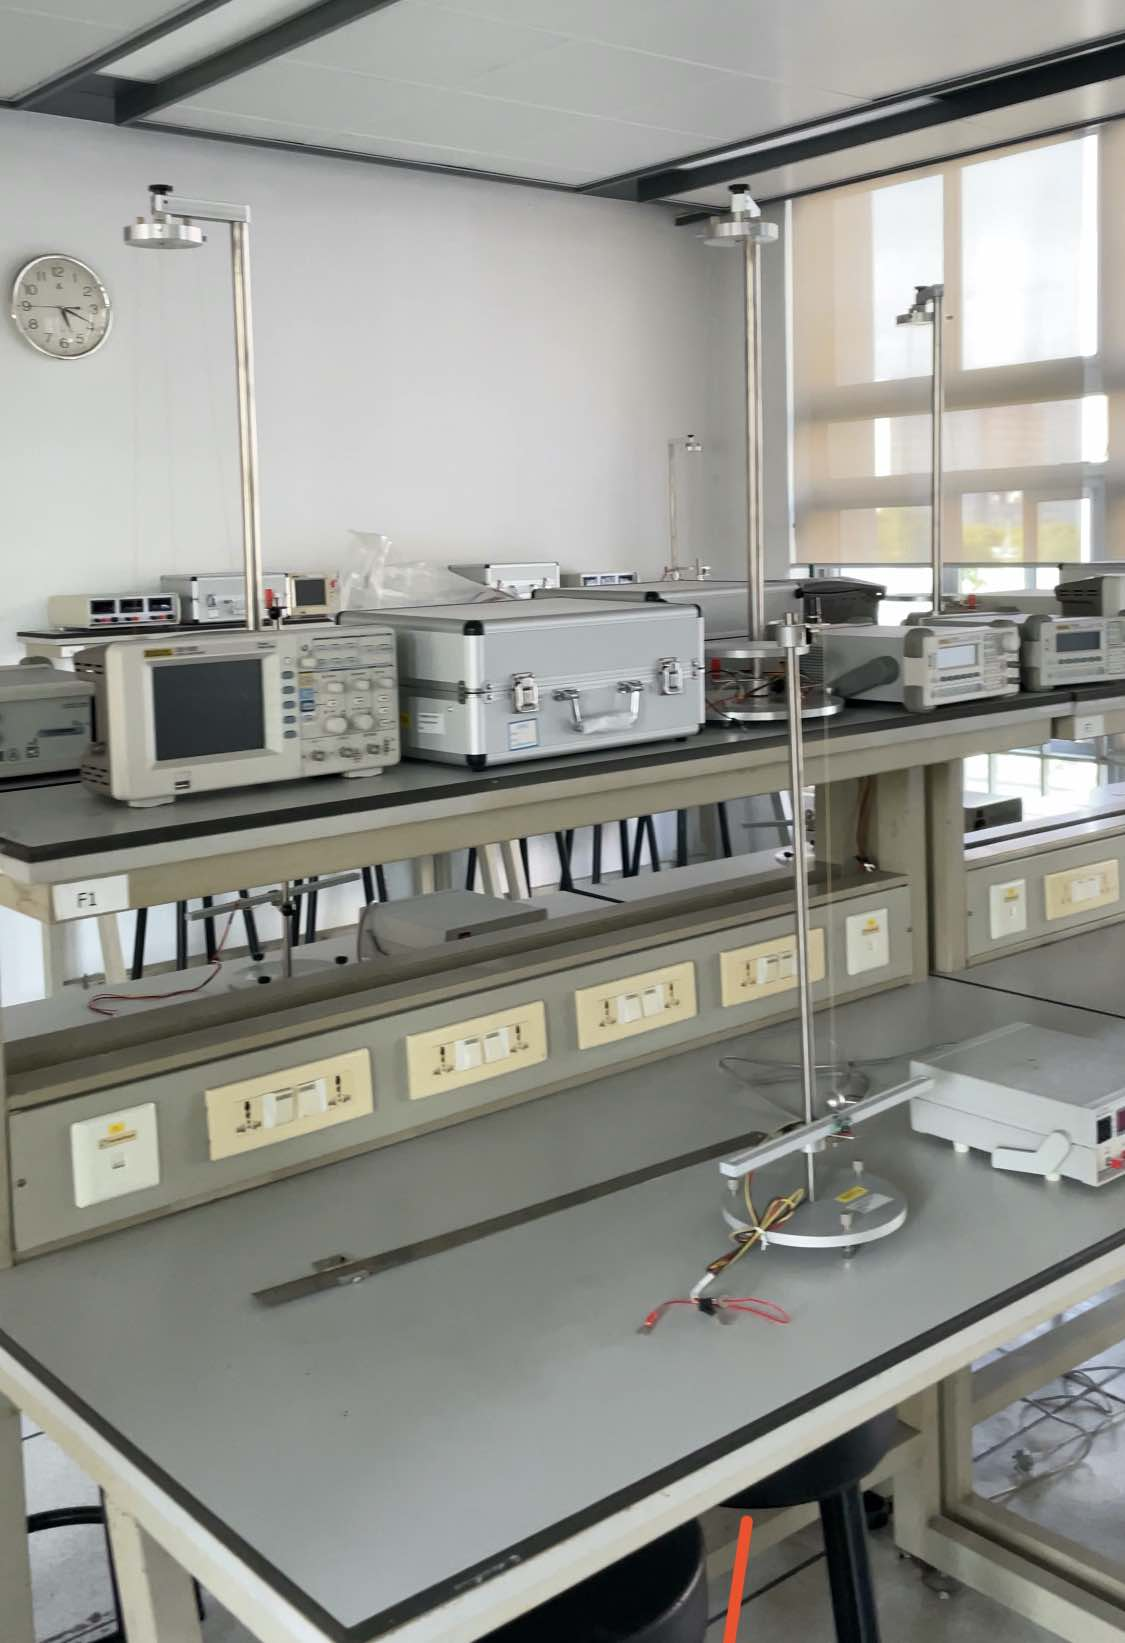
\includegraphics[width=0.95\columnwidth, right]{author-folder/Kai.Wu/lab.jpg}
    \end{figure}
\end{minipage}



\subsubsection{How to Conduct Tutorials}

\begin{enumerate}
    \item Prepare thoroughly before the class. When you stand on the podium, you are a teacher and must be responsible for everything you say and for the students. Copy the necessary materials to a USB drive before class, and log in to the classroom computer with your account to use it. You will also need to log in to systems like LMO and AMS. As the school computers are slow, arrive ten minutes early. Also, end the class ten minutes early to avoid complaints about going over time.
    \item Respond patiently to students’ emails and questions after class. Do not add students on WeChat lightly; ask them to contact you via email for any issues. Email is the official communication method in the school and protects the personal space and rights of teachers and TAs. There have been complaints about TAs not responding to students’ WeChat messages.
    \item Communicate with the module leader if you encounter difficult issues. Do not make decisions on your own; consult with the module leader. Share student feedback with co-teachers to improve the learning experience. Better student experiences lead to higher Module Questionnaire (MQ) scores. Good MQ scores can be included in your resume when job hunting.
\end{enumerate}

\begin{flushright}
    (October 30, 2022 by Yue Zhou) \\
    (Translated by GPT)
\end{flushright}

\subsection{TA Salary and Payment}
In 2022, the TA salary is 60 yuan per hour, paid monthly, with the salary for January work paid at the end of February.

\emptyline{}
Additionally, proctoring midterm and final exams is also considered TA work and will count towards scholarship students’ TA hours. Self-funded students are usually paid a higher hourly rate for proctoring. See the next section for more details on proctoring.

\begin{flushright}
    Translated by GPT
\end{flushright} \clearpage

\section{How to Invigilate Exams}

\subsection{How to Participate}
If a fully funded PhD student has not completed the required TA hours, the college will assign you to invigilate exams. There are only two invigilation sessions per semester: midterm and final exams. Due to the pandemic in recent years, there haven't been in-person exams for a while.

When there are many exams and not enough staff or fully funded PhD students, non-fully-funded PhD students can also sign up to be invigilators. The specific method is to wait for the school's email invitation, which will include a link for you to choose your preferred time. After selection, you can check your specific invigilation schedule on e-bridge in a few days.

The invigilation wage rate in 2022 is 60 RMB per hour. The preparatory work is minimal, and during invigilation, you basically just walk around. It's relatively easy and a good way for non-fully-funded students to earn money.

\subsection{Specific Steps}
First, the school provides invigilation training, which can be found under "Assessment and invigilation" in the email titled \textit{Teaching Assistant (TA) Training Programme}, or you can check your LMO. If you've never attended before, you might consider attending to get a general idea of the process.

An exam hall's invigilation is divided into senior invigilator (staff) and invigilation assistant (PhD students).

I've summarized the invigilation process as follows:
\begin{enumerate}
    \item The invigilation training mentioned above, although you don't have to attend every time, it's customary to receive the [invigilator ID badge] during each semester's training. You must wear it during invigilation and return it afterward. So even if you don't want to attend, you at least need to go once to get your badge. If you're lazy (like me), you can usually have other colleagues who are also invigilating pick it up for you (usually one person from the office collects all badges).
    \item Check your invigilation schedule on e-bridge, as shown below:
        \begin{figure}[H]
            \centering
            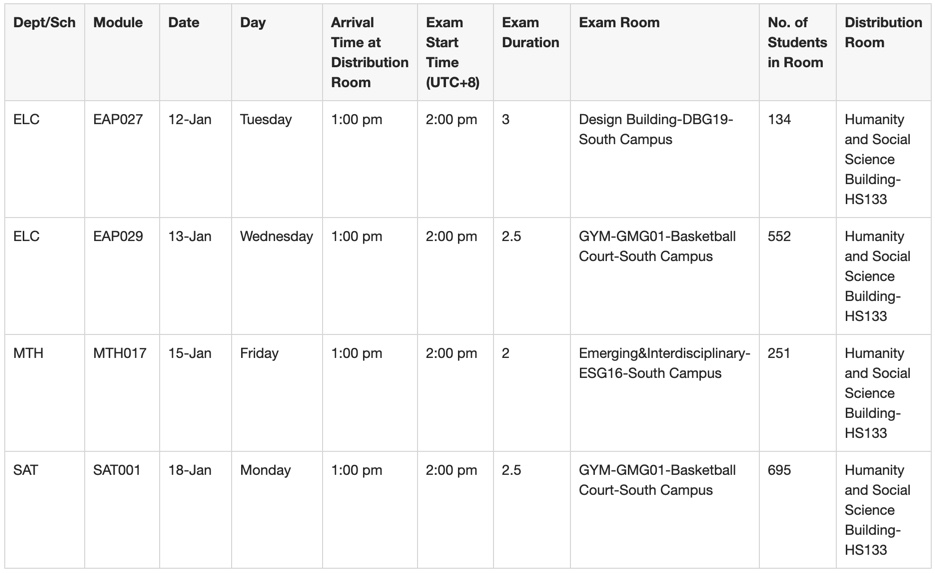
\includegraphics[width=0.5\columnwidth]{author-folder/Kai.Wu/invigi-table.jpg}
        \end{figure}
    \item First part of invigilation: pre-exam preparation. Before the exam starts, pay attention to the two columns in the table above: "Arrive Time at Distribution Room" and "Distribution Room". At the specified time, go to sign in and collect exam papers in advance. You will then get MCQ cards, answer booklets, exam attendance lists, small white cards, clay, and other materials to take to the exam hall.
    \item Upon arriving at the exam hall, the first task is to post materials. In the list of examinees, there is a version sorted by student number to be posted on the door for students to find their seats (other versions sorted by seat number are for invigilators). Separate each page of this list and use clay to stick them on the exam hall door or wall.
    \item Then start distributing answer booklets and answer sheets according to the seating plan.
    \item Generally, there will be multiple invigilators in an exam hall. When other invigilators arrive, assign some of the tasks of distributing answer booklets and sheets to them. Then, discuss with them to assign each person a specific area to be responsible for, including invigilation patrols and collecting materials.
    \item The chief invigilator (the teacher) will bring the exam papers, and you can help the teacher distribute them. If the chief invigilator hasn't arrived 20 minutes before the exam starts, you need to contact the teachers in the invigilator WeChat group to remind them.
    \item All materials (exam papers, answer sheets, MCQs, etc.) must be distributed 15 minutes before the start. Allow students to enter the exam hall 15 minutes before the exam.
    \item When multiple invigilators are present, generally leave at least one invigilator at each entrance to check student IDs. Students without student IDs or ID cards are not allowed to enter. Other invigilators can walk around inside the exam hall, paying special attention to ensuring students do not open the exam papers before the exam starts. If discovered, you need to stop it immediately. If there are many students doing this, ask the chief invigilator to warn them. To prevent loss, students' backpacks should not be placed outside the exam hall; they should be placed at the front or back of the hall.
    \item After the chief invigilator announces the start of the exam, for your responsible area, record any late-arriving students. You can note this on your invigilator attendance list.
    \item After the exam starts, walk around freely and exercise your authority as an invigilator. Focus on checking students' belongings to see if they have cheat sheets on their hands or paper slips. During invigilation, you are not allowed to use your phone or chat; you need to observe whether students are cheating. If cheating is encountered, you need to point it out on the spot, stop the student's exam, and make a note on their exam paper.
    \item 30 minutes after the exam starts, collect the small white cards (a card specifically for writing names, student numbers, etc.). After collecting, record the absent students in your area.
    \item If students need to borrow pens, pencils, or erasers, ask the chief invigilator how to handle it. If a student needs to go to the restroom, an invigilator needs to accompany them (just to the restroom entrance is sufficient), and accompany them back. In principle, only one student can go to the restroom at the same time. If a second student needs to go, they must wait until the first student returns.
    \item Finally, when the exam ends, collect all materials, including scratch paper (if any). Students must wait until you have finished collecting and counted everything accurately before they can leave.
    \item After the exam, tally the number of attendees, late arrivals, and absentees, and have the chief invigilator record it on the record sheet. Finally, there are two sheets that require the signatures of all invigilators. Only with these two signatures plus the initial sign-in will your work be successfully recorded.
    \item Then it's time to say goodbye. The invigilating teacher will take away the answer booklets and MCQs. You need to return the two signed sheets and all materials the chief invigilator didn't take (including exam papers, scratch paper, etc.) to the place where you initially signed in. If this is your last invigilation of the semester, you need to return your invigilator ID badge.
\end{enumerate}

\emptyline{}
Finally, I'd like to share a checklist I use after invigilating more than a dozen times:

\begin{enumerate}
    \item When picking up materials, check the number of invigilators to facilitate dividing areas.
    \item Post the seating charts at the exam hall.
    \item Confirm with the teacher:
    \begin{enumerate}
        \item Should the answer booklets be collected in order? If yes, at the end of the exam, do not let students pass the papers; absent students and those who submit early should also leave their papers on the desk.
        \item Stickers? If needed, have students attach them at the end of the exam.
        \item Whether to record restroom visits and start/end times.
        \item How to handle absentees (fill in information on the small white card and answer booklet, write "Absent" on the answer booklet).
    \end{enumerate}
    \item After receiving seat numbers, divide areas according to the number of invigilators. The roles in each area include everything except collecting papers:
    \begin{enumerate}
        \item Before the exam: Distribute papers, check if students are seated correctly, ensure students do not open the white question booklets.
        \item Letting students in: Check student IDs at the entrance.
        \item First 30 minutes: Check seating, record late arrivals.
        \item At 30 minutes: Record absentees, collect small white cards, then fill in the student attendance sheet.
        \item Restroom visits: Record seat number, start and end times.
        \item 15 minutes before end: Record seat numbers and count of students who submit early.
    \end{enumerate}
    \item Before finishing: Remind the teacher to have students attach the answer booklet.
    \item After finishing: Collect answer sheets in order, count your own portion, then combine and randomly count a portion.
    \item Summary list: Number of students, absentees, early submissions, remaining, special cases.
\end{enumerate}

\begin{figure}[H]
    \centering
    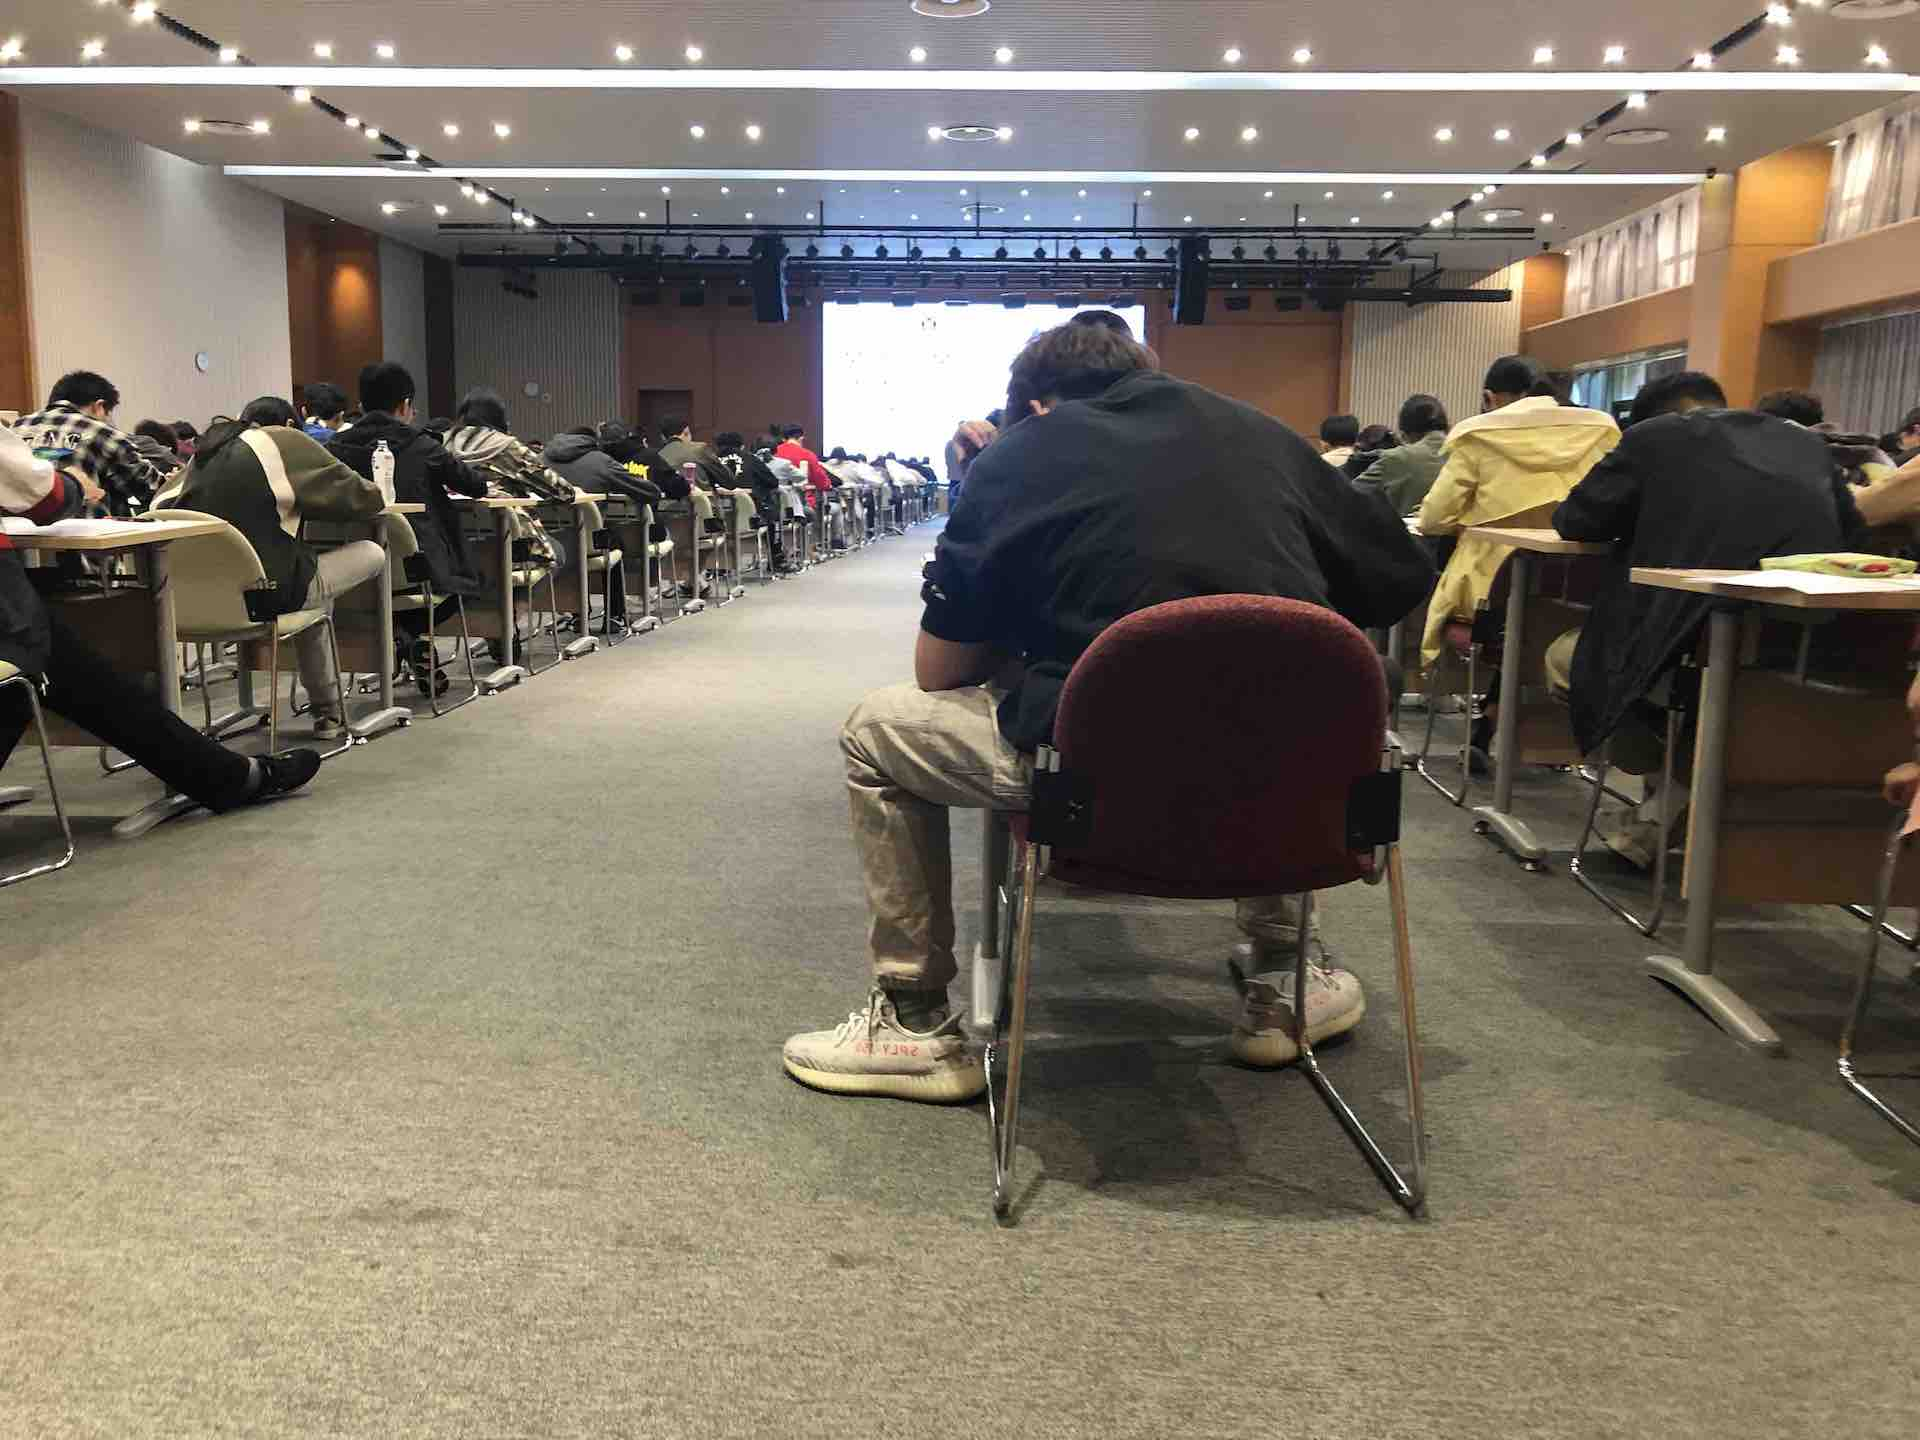
\includegraphics[width=0.9\columnwidth]{author-folder/Kai.Wu/invigilation.jpg}
    \caption{November 15, 2020, an exam hall on the G floor of the CB building, during invigilation}
\end{figure}

\begin{flushright}
    (October 22, 2022 by \Wu)

    (Major update: December 30, 2022 by Yue Zhou) \\
    (Translated by GPT)
\end{flushright}

% \begin{figure}[H]
%     \centering
%     \includegraphics[width=0.5\columnwidth]{author-folder/Kai.Wu/}
% \end{figure}

% \usepackage[export]{adjustbox}

% \item 
% \begin{minipage}{0.3\textwidth}
%     Text
% \end{minipage}
% \begin{minipage}{0.63\textwidth}
%     \begin{figure}[H]
%         \includegraphics[width=0.4\columnwidth, right]{author-folder/Kai.Wu/}
%     \end{figure}
% \end{minipage}

% \input{author-folder/Kai.Wu/.tex}
 \clearpage

\section{学位论文,论文答辩,和毕业}
\label{sec.thesis_viva_graduation}

你想毕业吗?你想成为Doctor吗?那就赶快看这里吧!只要一篇一百多页的论文,毕业不是梦!\sout{(发癫结束)}

\subsection{官方流程和时间线}
\label{sec.official.flowchart}

正如本攻略的宗旨是官方资料的补充,首先请尽量熟读下图的官方毕业流程,里面的时间线、条件和顺序都是万分准确的。

\begin{figure}[H]
    \centering
    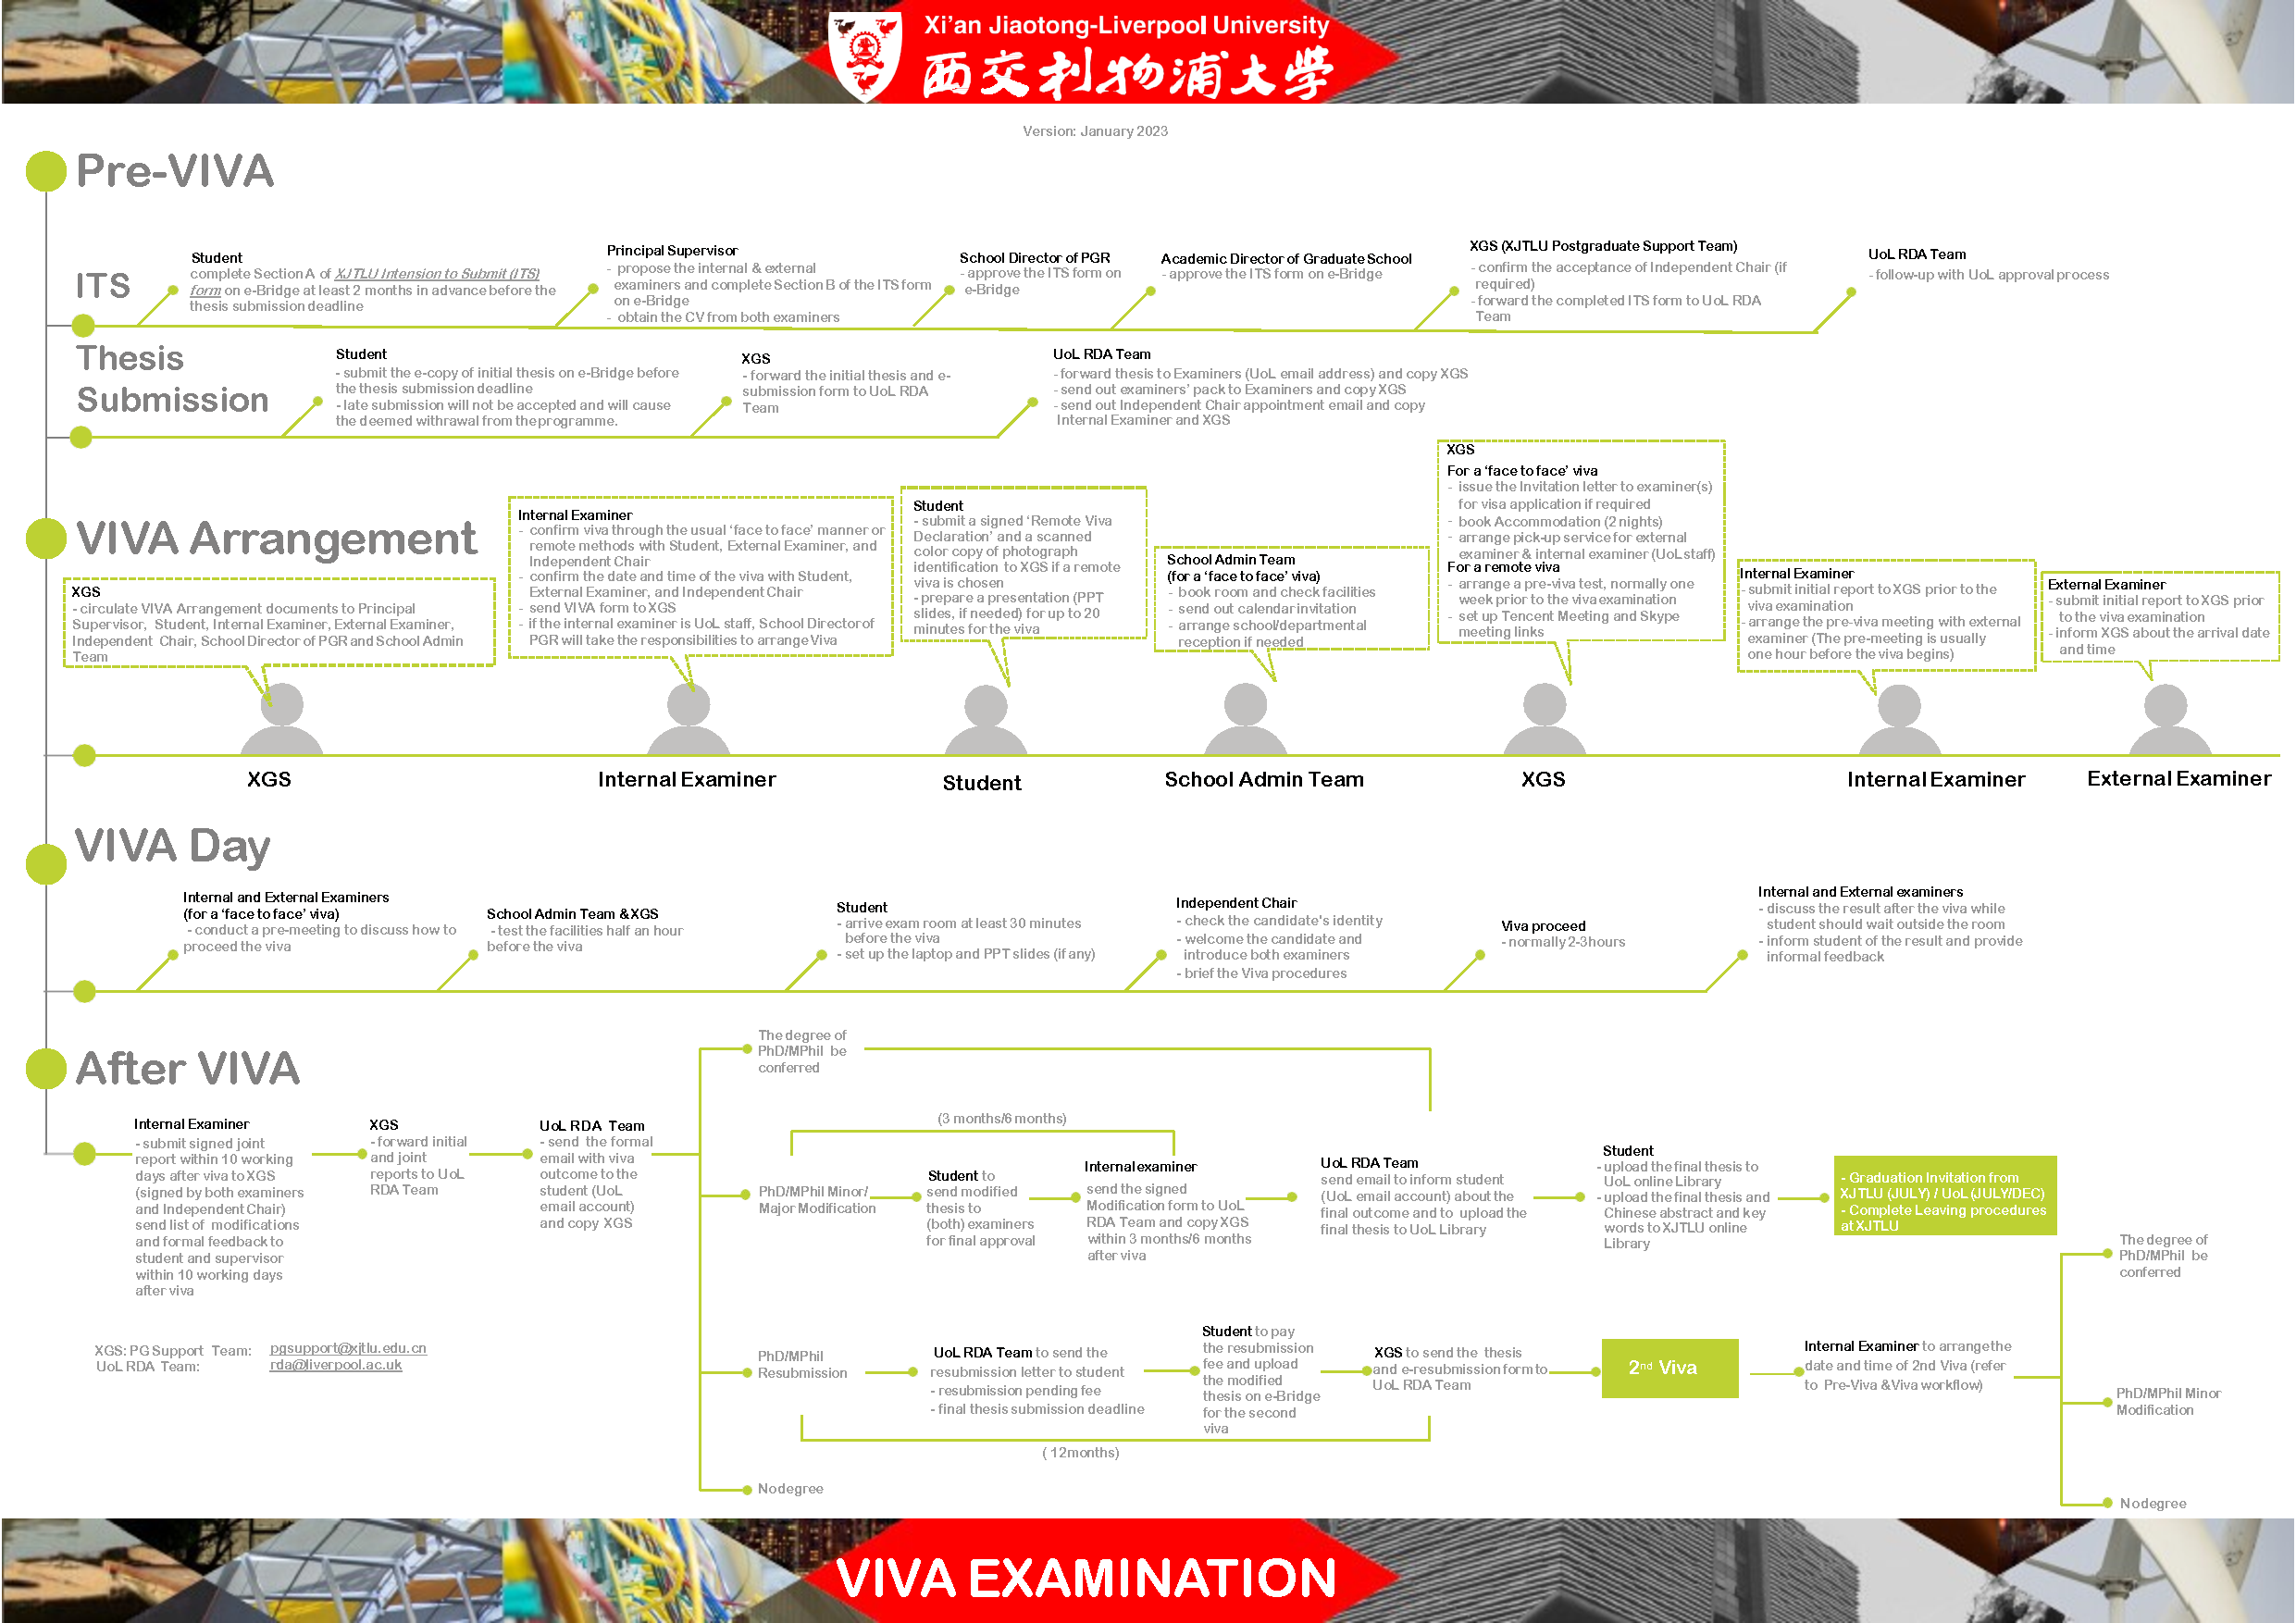
\includegraphics[width=\columnwidth]{fileshare/XJTLU VIVA Examination Arrangement Flowchart_2023.pdf}
    \caption{官方的毕业流程图。单独的文件可在fileshare里找到\url{https://gitee.com/kaiwu-astro/xp_pgrs_unofficial_guide/tree/main/fileshare}。注:我还真不知道这个文件在哪里下载的,这是我导发我的,想要最新版的可以在ebridge里找一下}
\end{figure}

如果想直到每个步骤大概要花多少时间,跳转章节 \ref{sec.graduation.time}。

\subsection{ITS: Intention to submit}

Q:ITS重要吗,我着急写论文呢,暂时不管它行不行

A:如果你对毕业时间有要求,请务必谨记尽早提交ITS表!ITS是你的论文和答辩一切程序的开始。现有规定,你的论文只能在\textbf{提交ITS之日起+2个月之后}才允许提交,可以延后,但不允许提前。(ITS提交后,一年内必须交论文;和你本身的论文deadline共同作用,以早的那个为准)

Q:ITS里面会填什么

A:毕业论文的题目、毕业论文的摘要、基本个人信息。题目和摘要不需要是最终决定的版本,也就是后面可以改。

Q:那我随便起个题目和摘要,走个过场行不行啊

A:这个表的作用是:导师和研究生院会拿着这个标题和摘要去决定你的内审、外审。这个题目和摘要也会发给他们。因此,和最终版可以有修改,但是也要尽量准确的反映你这几年的研究。

Q:我还要问

A:先看看官方文件:\url{https://www.liverpool.ac.uk/aqsd/academic-codes-of-practice/pgr-code-of-practice/}

\subsection{Thesis: 学位论文/毕业论文}

\subsubsection{格式和排版}

官方文件:\url{https://www.liverpool.ac.uk/media/livacuk/tqsd/code-of-practice-on-assessment/annex-7.1-PGR-CoP.pdf}
<-- 一切对格式不确定的请以这个为准。下面是微信群里的一些日经问题。

Q:可以用什么软件写毕业论文?

A:根据上面的规定,利物浦对软件没有要求,也就是你想用什么都可以。常用的有:Microsoft Word, \LaTeX

Q:推荐用什么软件呢

A:\LaTeX 优点:(1)非常方便输入公式,(2)参考文献和引用处理起来非常方便,不需要Endnote等外部软件辅助,(3)格式美观,风格统一,排版很难难看,(4)文件小,文件可分散,方便备份。\LaTeX 缺点:学习成本较高。如果你们专业发期刊论文/会议论文都不用\LaTeX 而用Word,那你切换过来就要花些时间学习。

Q:上面这个排版要求文件要求好多好细,呜呜呜给我一份毕业论文模板吧呜呜呜呜

A:
\begin{enumerate}
    \item Word还真的有一个官方模板,可以在本项目fileshare下载\url{https://gitee.com/kaiwu-astro/xp_pgrs_unofficial_guide/tree/main/fileshare}。来源:ELC Thesis Writing Camp的老师
    \item \LaTeX 没有官方模板,但数理学院(SMP)的大部分毕业生都是用\LaTeX 写的毕业论文。可以直接在Overleaf模板库直接搜索Liverpool Thesis,应该只有一个搜索结果,采用即可。
    \item 请使用模板的同学特别注意,never fully trust the template! Word模板是西浦ELC的老师给的,不是利物浦给的;Overleaf更是民间模板。理论上,他们对你的论文和毕业都\textbf{不负责}。因此拿到模板过后,第一件事永远还是打开上面的Code of Practice,一条一条的比对看是否达到了要求。
\end{enumerate}

\subsubsection{字数}

Q:上面的CoD只说了一个字数上限,那最低字数要求呢?

A:另一个日经问题。我曾经在研究生院Thesis Writing Camp课程上问了老师,他的意见是,西浦Master thesis的字数上限是3w,因此PhD thesis最好超过这个数。但我后来发现不是这回事。我见过有的论文不到100页,有的接近200页,都毕业了。从全校来看,这个是真的没有要求。你如果不放心,还是想对最低字数有点数,很简单,去利物浦图书馆和西浦图书馆下载毕业论文,重点参考你们学院、你们系、你们专业、最好直接是你同门已毕业同学的毕业论文,有多少字有多少页。\textbf{请谨记,字数多并不能保证你能轻松毕业}。我的一个师兄thesis就是接近200页,吃了个大改,外审说他写得太多了像教科书。

\begin{flushright}
    (2024年08月12日 by \Wu)
\end{flushright}

\subsection{Thesis Defense}

\subsubsection{Pre- and Post-Defense Process}

\begin{enumerate}
    \item At least two months before officially submitting your thesis on e-bridge, have your supervisor select a list of potential examiners for your upcoming defense. Submit this list to XJTLU's pgsupport and the University of Liverpool for review and approval.
    \item After officially submitting your thesis on e-bridge, the university will contact the respective examiners and then reach out to you to confirm the defense date and format (the defense typically occurs within 1-3 months after submission. The format can be either online or offline — confirm specifics with pgsupport).
    \item Generally, there will be a rehearsal before the defense to test the network and PPT presentation. You can also request time to practice your presentation in the designated conference room.
    \item Before the defense, the examiners will hold an internal meeting, usually on the same day (though sometimes earlier). They will then invite you into the meeting room to officially start the defense. Besides the two (or three under special regulations) examiners, there will be an observer (responsible for overseeing the overall process, arranging breaks, and addressing any procedural questions you might have). During the formal defense, the observer typically does not speak. If you have any questions, feel free to ask them.
    \item After your PPT presentation, there will be a Q\&A session. Depending on the circumstances, this can last from 1.5 to 3.5 hours (historically, there have been instances lasting up to 7 hours). Once the Q\&A concludes, you will be asked to leave the room temporarily while the examiners deliberate. After about 10-15 minutes, you'll be invited back in and informed of the results.
    \item The examiners' revision report will be sent to you within 10 working days. Based on their feedback, you'll need to make the necessary revisions within the specified timeframe and submit them to the primary examiner for confirmation.
    \item Once everything is confirmed, upload the final version of your thesis to complete the process.
\end{enumerate}

\begin{flushright}
    July 5, 2024 by Ziwen Xie \\
    GPT translation proofread by \Shiyao
\end{flushright}

\subsubsection{How to Prepare for a Viva}

Experience from the School of Science:

\textit{Try not to cram everything into a couple of days. Spreading out your preparation helps maintain a good state of mind daily, which is crucial for performing well during the actual defense.}

\textbf{1. Thoroughly read your thesis word by word as if you are a new reader, considering the following questions as you go:}
\begin{enumerate}
    \item Are any paragraphs unclear?
    \item Can you fully grasp and independently explain specific concepts?
    \item Do you understand the relationships and differences between chapters and the internal logic of the overall structure?
    \item Are you aware of the internal logic between sections within chapters and the sequence of experimental designs?
    \item What issues can each experiment address individually or collectively? What conclusions can be drawn from each major chapter?
    \item Do you fully understand the algorithms, models, and basic concepts cited from the literature? How are they connected to your core research objectives?
    \item Are there any previously unnoticed expression errors or chart inaccuracies that need correction?
    \item What is the purpose of your research? What motivated the choice of your methodology? How does it have advantages over other methods?
\end{enumerate}

\textbf{2. After organizing these points, analyze each chapter (including the abstract) in detail:}
\begin{enumerate}
    \item Can you summarize the background information in your own words?
    \item What does each subsection convey? Ensure consistency among subsections within a chapter.
    \item Highlight the key points or core logic of specific experiments or experimental designs.
    \item Understand the progression, parallelism, or other relationships and differences among experimental results (e.g., Experiment A demonstrates 'a', which serves as the foundation for Experiment B—this is progressive. If 'a' and 'b' are similar, then A and B are parallel).
    \item Justify the selection of experimental subjects and models (including why other related subjects or models weren't used).
    \item Based on your results, what future experiments could be pursued? (This may include why certain experiments weren't conducted, reasons for future experiments, potential outcomes of future experiments, foundational assumptions, and practical challenges—which explain why they weren't done in the current phase but were considered).
    \item Ensure the abstract includes key results and innovations.
\end{enumerate}

\textbf{3. Key Points for Preparing Your PPT and Viva:}
\begin{enumerate}
    \item Allocate 20 minutes into four sections: background introduction, experimental setup, experimental results, and conclusions—in approximately 5 minutes each. You can shorten the first three sections since the examiners have already read your thesis.
    \item Print your thesis and bring it with you to the defense. Take notes during the Q\&A session (this also gives you brief moments to compose yourself).
    \item Include essential figures and results in your PPT with concise descriptions.
    \item You don't need to discuss the challenges you faced or focus on future experiments or designs (examiners may ask about these, or you might mention them when answering questions). Depending on the situation, you can omit this from your PPT to save time.
    \item Ensure your PPT runs smoothly, and all text and images are clear. During practice sessions, simulate the actual presentation scenario as closely as possible.
    \item Remember to drink water during the defense—sip slowly and frequently. Eat some high-energy, easily digestible food beforehand. If you're not hungry, consider a chocolate bar or an energizing drink. Arrive early to familiarize yourself with the environment, which can help calm your nerves (and don't forget to visit the restroom beforehand).
    \item When answering questions, feel free to reference any part of your thesis. Some points in earlier chapters may connect with later ones or relate to future plans and final conclusions. If an examiner asks something you're unsure about or haven't considered, it's okay to admit it. Express your willingness to explore it further and ask for guidance or references in their feedback to assist with your revisions.
    \item Typically, each question and answer lasts about 3-5 minutes. With two examiners, handling around 20 questions each is substantial. Usually, the defense lasts between two to two and a half hours, with breaks in between (but once you're engaged, you might lose track of time).
\end{enumerate}

\textbf{4. Non-Thesis Related Questions:}
\begin{enumerate}
    \item How can artificial intelligence and ChatGPT inspire your research?
    \item Can your research be applied to other types of data, diseases, or fields? Why?
    \item What do you think are the shortcomings in your field?
    \item What is your biggest takeaway from your doctoral studies?
    \item If you had to do it all over again, would you still choose to pursue a Ph.D. and undertake this project?
\end{enumerate}
Tips: It seems the examiners are just curious and want a chat. Relax and answer accordingly. \textbf{Finally, according to data from a pgsupport staff member, there has never been a failed defense since our university was established. So, don't worry too much—just perform as you normally would. Good luck.}

\textbf{5. Ask your supervisors if they can help you anticipate potential questions. If time permits, see if they can arrange a mock viva for you (optional). It's also beneficial to consult recent graduates about their defense experiences, as certain aspects may change yearly.}

\begin{flushright}
    July 5, 2024 by Ziwen Xie \\
    GPT translation proofread by \Shiyao
\end{flushright}


\subsection{我想尽快拿学位证!如何速通毕业流程}

急急急,你就是急急国王。下面是一个合格的急急国王必须知道的事。

\subsubsection{毕业的证明文件}

\begin{enumerate}
    \item 完读证明(Completion of Studies Certificate),由西浦研究生院开具。证明内容:已提交毕业论文,已通过答辩,即将在XXXX年X月的毕业典礼上授予博士学位。我的Example:
    \begin{figure}[H]
        \centering
        
\includegraphics[width=0.8\columnwidth]{author-folder/Kai.Wu/Completion_of_Studies_Certificate_EXAMPLE.jpg}
        \caption{仅供参考,因此加上了巨大的example防止非法盗用}
    \end{figure}
    \item 学位证(aka PhD degree, degree certificate)。注意!利物浦规定,学位只会在\textbf{利物浦}毕业典礼上颁发,而利物浦毕业典礼一年只有两次,一般是7月某天和12月某天。如果你不去利物浦毕业典礼,会在毕业典礼前后先给学位证的电子版(有法律效力,可办中外合办认证),然后原件慢悠悠的邮寄到西浦。
    \item 中外合办学位认证。拿到电子学位证即可办理 \url{https://zwfw.cscse.edu.cn/}。持有该认证,你的利物浦学位就在中国境内被教育部承认。
\end{enumerate}

因此,首先确定你要去的公司/单位能接受哪种证明文件。最松的情况,你答辩完收到利物浦确认的Pass (with minor/major modification)邮件就行。也有能接受完读证明的。如果对方比较死板,不见学位证就不行,甚至没有中外合办认证也不行,那就要特别规划好毕业进度,因为每年只发2次证!

\subsubsection{学位证:最关键时间节点}

如果你确定不需要赶时间拿学位证,那本节接下来的都可以忽略,因为完读证明任何时候都可以开。

Q:我能否在7月/12月毕业?硬性要求是什么?

A:最好的方式是直接上利物浦网站查询,或者直接google liverpool phd graduation。过去几年的要求都是:在某个时间点之前,利物浦图书馆确认收到你的\sout{终极完全不改版的}最终论文。例如,如果要参加2024年7月15日的利物浦毕业典礼(在这一天颁发学位证,或邮寄),需要在2024年6月25日之前,利物浦图书馆确定收到了最终论文。这份论文是你的内外审都满意、同意的最终版。如何走到这一步?看下一节。

\subsubsection{每个步骤要等多久?如何预估时间?}
\label{sec.graduation.time}

以下完全基于已毕业同学的经验整理。新毕业的同学,请不吝赐教,补充你的真实案例。

以 \ref{sec.official.flowchart} 中提到的流程图来梳理:
\begin{enumerate}
    \item ITS:你提交过后其实就不用管了,专心写论文吧,剩下的都是导师和研究生院的活。背后的流程:i. 导师propose内审老师、外审老师; ii.研究生院审核,可能因为觉得这个老师和你利益相关等原因驳回其中的某人,然后你导师重新propose,直到研究生院满意为止,定下来内审外审人选各一个。在这个阶段,严格来说你直到论文提交都不能直到内外审老师是谁,导师需要保密,所以也不要\textbf{太}为难你导师去问是谁。
    \item 首次论文提交 到 论文答辩:(30天±30天)提交后,西浦研究生院(XGS)和利物浦学位办(RDA)会花两三个工作日简单处理下论文,发给内外审。\textbf{内审}一旦收到论文,就负责安排答辩时间。也就是说,你的答辩日期完全取决于你+内审+外审+独立主席(independent chair)都有空的某个时候(正常2-3小时)。因此,最早答辩日 = 论文交了过后三四个工作日;最晚答辩日则没有规定,找到四个人有空的时间为止。如果你赶时间,你能做的:(1)论文提交过后,尽早找你的内审,催ta安排日期;(2)把你论文提交过后一两个月的日程尽量腾空,不要因为自己的日程耽误答辩;(3)内外审一旦决定就不好更换,但独立主席容易换(有时会出现答辩一周前主席没空,找人另一老师顶上的事情),如果你们四个人里面是主席时间不合适导致拖很晚,尽早找你导师看能不能换主席。正常来说:交论文+60天=答辩 算非常慢的(但也有例子,据说是交论文前后不巧遇到了利物浦搞罢工)。一般会在+30天左右。
    \item 答辩完成 到 最终论文通过:(0 - 180天,典型为3-4周)。根据答辩结果不同这一步会有很大区别。(1) Pass (无条件) = 0天,论文初版即为最终版。(2) Pass with minor modification (小改),绝大部分同学都是这个结果。(3)Pass with major mofication(大改)(其他比较惨的情况很少,\sout{建议让导师和他举荐的examiner打一架})。如果是2或3,内外审会在10工作日(=2周)内出具书面的修改报告。这个过程个人建议不要催,他们要交的表和报告不少。之后就取决于你能多快改完论文。改完过后,按利物浦邮件指示,把改好的论文用指定的方式发给老师。这一步完全取决于你的内外审老师多久能respond,以及他们对你的修改是否满意。因为按照流程,如果不满意,他们有权让你改到他们满意为止。为了避免反复迭代,建议和导师反复斟酌新文本,争取一次搞定。这个版本的论文不会自动作为最终版,你可以在里面用颜色或者加粗标注修改过的地方,方便两位老师查阅。
    \item 最终论文通过 到 利物浦图书馆确认收到:(7天)这一步只是行政手续。在通过后,RDA会发邮件通知你上传最终论文(我的情况:内审老师告诉我[他们已告诉XGS和RDA修改版通过],过了4天收到上传通知),然后你将最终论文发送给利物浦,过几天(我的情况:2天)就收到利物浦图书馆正式通知邮件,论文成功上传。
    \item 实际还有一些手续,比如西浦会也让你上传一份到西浦图书馆,不知道是否会影响毕业,收到通知过后也最好尽早完成。
    \item 电子degree:具有法律效力的电子版degree会在你毕业典礼日期的前后几天内颁发。按照利物浦给你的邮件,在verify.liverpool.ac.uk里查询。
    \item 纸质degree:如果你人去利物浦参加毕业典礼,那就是现场领取。如果你不去,会在你毕业典礼日期后官方邮寄到西浦,等就完事了。我的情况:7月15日利物浦毕业典礼(人没去),纸质版7月30日寄到了研究生院。如果到时候人已经不在学校,可以委托研究生院邮寄(不推荐,丢件没法补,风险自担)。
\end{enumerate}

\begin{flushright}
    (2024年08月12日 by \Wu)
\end{flushright}

\section{Important Information Related to Employment}

Regarding student status, academic qualifications, employment materials, etc., it is recommended to first read the FAQ at the school's career center: \url{https://careers.xjtlu.edu.cn/Dispatch/Home/Master}

\subsection{Student Status and Xuexin Network?}

During our study period, student status cannot be found on the Xuexin Network, but it can be checked on the Ministry of Education's Sino-foreign Joint Program Supervision website: \url{http://rzzccx.crs.jsj.edu.cn/}. Therefore, don't think about student discounts like Haidilao's university student discount that requires Xuexin Network verification—you won't be able to enjoy them. There is a chance to enjoy benefits at the Apple Store; policies vary each year, so it is recommended to call the Apple Store directly to inquire.

After graduation, your Liverpool degree must be authenticated by the Ministry of Education to be recognized by the Ministry of Education. See Section \ref{sec.thesis_viva_graduation}

\subsection{Transcripts?}

Unlike domestic doctoral programs, we do not have transcripts upon graduation. Transcripts correspond to the "HEAR report" at Liverpool, but some students have asked Liverpool officials and were clearly told that PhD students do not have HEAR reports. If your employer rigidly requires a transcript, you can email Liverpool to inquire.

\begin{flushright}
    (August 12, 2024 by \Wu) \\
    (Translated by GPT)
\end{flushright}

% \begin{flushright}
% ( by Kai Wu)
% \end{flushright}

% \begin{figure}[H]
%     \centering
%     \includegraphics[width=0.5\columnwidth]{author-folder/Kai.Wu/}
% \end{figure}

% \usepackage[export]{adjustbox}

% \item 
% \begin{minipage}{0.3\textwidth}
%     Text
% \end{minipage}
% \begin{minipage}{0.63\textwidth}
%     \begin{figure}[H]
%         \includegraphics[width=0.95\columnwidth, right]{author-folder/Kai.Wu/}
%     \end{figure}
% \end{minipage}

% \input{author-folder/Kai.Wu/.tex}






% %# -*- coding: utf-8-unix -*-
%%==================================================

\chapter{Other Guides}

\begin{flushright}
    ——Take a glance, no loss; take a second look, huge gain
\end{flushright}

\section{大坑:假如明天你突然丢失电脑所有数据怎么办?——如何备份资料}

\begin{figure}[H]
    \begin{tabular}{rl}
        
\includegraphics[width=0.5\columnwidth]{author-folder/Kai.Wu/backup1.jpg} &
        
\includegraphics[width=0.4\columnwidth]{author-folder/Kai.Wu/backup2.jpg}
    \end{tabular}
    \caption{\href{https://baijiahao.baidu.com/s?id=1719578217211021768}{链接:贵阳一女大学生8000字毕业论文保存失败崩溃大哭}}
\end{figure}

绝大部分同学本科就买了自己的电脑。虽然自己的各种作业资料,到现在博士阶段的研究数据、论文,全部就只存放在这一台电脑里,但并没有足够意识到自己电脑的重要,和保存在电脑里信息的脆弱。每年,都会有如上图的事情发生,给当事人带来上新闻被全国人民笑话的沉重打击。

丢失一篇正在写的论文,其实是小事,毕竟研究资料全部都在。上面新闻的当事人,其实也就用了几天时间就重新写好了论文。但那些万年不动、又极其重要的资料,又是绝对安全的吗?

想象一下,假如
\begin{itemize}
    \item 你某天手一滑,电脑摔倒地上,再也开不了机,硬盘也没法恢复
    \item 头昏脑涨的一天,你接了一杯咖啡,一不注意,咖啡撒在了电脑上,瞬间短路,电脑滋滋冒油
    \item 你不慎点击了一个链接,中了勒索病毒;或者,西浦内网被网络攻击攻陷,所有电脑中勒索病毒。你的所有文件被加密封锁。
    \item 你把电脑带出去办公或者采集数据,整个电脑直接被偷走
    \item 你过年回家,在路上,背包或者行李箱被人偷走了或者拿错了
    \item 无恶意,但万一,西浦着火了,西浦进水了(MB的5楼一下大雨就漏水),西浦楼塌了,撤离的时候你根本来不及拿电脑
\end{itemize}


\begin{figure}[H]
    \centering
    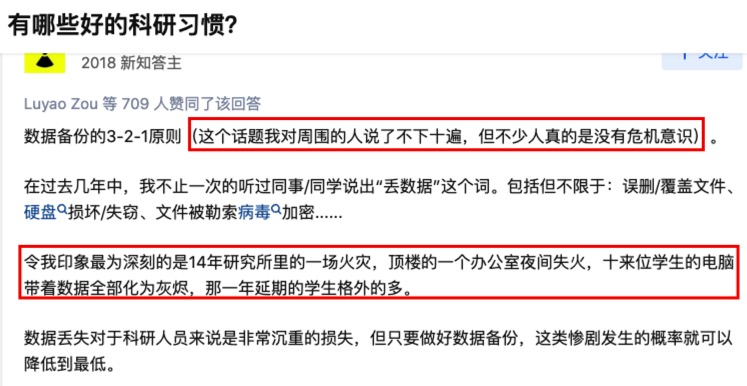
\includegraphics[width=0.8\columnwidth]{author-folder/Kai.Wu/backup_zhihu.jpg}
    \caption{\url{https://www.zhihu.com/question/394796969/answer/1501840215}}
\end{figure}

这些情况,单个可能很罕见,但所有可能性加起来,再乘以3到4年时间,至少发生一次的概率并不小。如果发生,你的博士进度会被耽误多久,你的青春又会被耽误多久呢。

只有一份的数据是非常脆弱的。现在思考一下,你赖以生存的电脑、数据、论文,是否只存了一份?如果是,请立即把屁股从椅子上挪起来,去厕所洗把脸,问问自己都是成年人了,怎么心这么大,然后开始看下面的攻略。

\subsection{理论:321原则}

「3-2-1 原则」是商业公司通用的数据备份金方法,具体内容是:
\begin{itemize}
    \item 3:存储 3 份完整文件,一份原件加上两份拷贝。
    \item 2:将文件起码保持在两种不同的介质上。
    \item 1:将一份拷贝保存在异地。
\end{itemize}

所谓的「介质」,是指内置硬盘、移动硬盘、U盘、网盘等不同的存储介质。说起来好像很麻烦,但对我们来说最简单的实践是:原件保存在内置硬盘,将两份拷贝分别存到移动硬盘和网盘,就同时达成了三条要求。这时,你回过头去看一下我上面列举的所有可能的灾难性问题(甚至即使是网盘公司突然倒闭),都能做到游刃有余,不影响你的科研!

\subsection{实践}

到动手准备的环节了。首先根据你手里的资源,决定你要备份的范围。最土豪的情况,你可以把整个电脑做一个本地备份 + 云端网盘备份,但很多时候,要么网盘容量很小,要么移动硬盘容量不够,要么网速太慢把太多资料传网上很慢,所以先划定你的备份范围。

\begin{itemize}
    \item 最经济的方案:只备份最重要的文件。例如:论文、科研资料、CV、电脑桌面,等等。网盘实时备份+移动硬盘定期备份。对移动硬盘和网盘容量要求都很小。
    \item 最高效的方案:整个电脑(包括最重要的数据)本地备份;最重要的科研、论文等加一分网盘实时备份。这需要一块比你电脑硬盘更大的移动硬盘(不贵),加正常容量(10个G左右)的网盘。
    \item \sout{最土豪的方案:买个NAS,插几十T的盘,组RAID1,再实时传一份到异地。}
\end{itemize}

正常电脑硬盘容量一般在2T内,另外我假设大家去买一块2T以上的移动硬盘(500块以内)应该压力不大(导师经费较多的,可以直接问导师要,直接说想要一块移动硬盘做备份问导师能不能帮忙买就行,2000块以内报销都很简单)。所以下面只介绍中间的高效的方法

\subsubsection{电脑整机备份}
\label{sec.pc_backup}

把电脑整机备份的一大好处就是,假设电脑直接灭失,新买一台电脑过后,能在一天之内完全恢复之前的工作状态,无缝衔接,科研毫不受影响。

Windows和macOS都自带系统级的整机备份方案。网上攻略特别多,我就不废话了。
\begin{itemize}
    \item Win请在b站直接搜索windows备份看教程,一般使用系统的“备份与还原(windows7)”(虽然名字里有win7但win10和win11也是完全能用的,这也就是为什么一直没被扔掉),比如看这个视频 \url{https://www.bilibili.com/video/BV1Dy4y1x7RP}
    \item macOS请在b站直接搜索mac time machine,一般使用系统设置里的“Time Machine”,比如看这个视频 \url{https://www.bilibili.com/video/BV1oy4y177qS}
\end{itemize}
一个视频看了不太明白没关系,多搜几个看,也同时善用谷歌、知乎等。初学者可能感觉学习成本有点高,但不要等到电脑炸了再开始准备呀。

\subsubsection{网盘备份}
\label{sec.net_drive_backup}

Box(\url{https://box.xjtlu.edu.cn/})是学校的自建网盘,2022年升级到了每人100G的免费空间,内网上传下载速度可达千兆,同时自带3个月的文件历史版本,秒杀一众网盘。把重要的文件夹拖入seafile客户端(不用移动文件夹),他就会自动实时备份到学校网盘。使用方法见 \url{https://guide.xjtlu.edu.cn/box/student/drive_client/drive_clent_for_windows.html} 。Box唯一的问题是不支持链接分享文件(老师有分享权限,我们没有),但作为备份网盘非常合适。

另外,如果对学校IT不放心,可以同时安装一个另外的商业网盘进行第二重网盘备份。个人严重不推荐百度云,因为偶尔会随机吃文件。国内的,我个人推荐坚果云(免费版无限空间,但限制每月流量),国外网盘推荐Onedrive(个人版免费5G,可在淘宝搜索onedrive扩容花几块钱扩容到永久15G)。另外,大家的利物浦账号下都有免费1T的Onedrive,羊毛薅起来(但注意毕业前得把数据迁出去,因为毕业了要收回账号),参见这一章节 \ref{sec.fuli_liverpool}。


\subsection{论文备份·文件历史版本}
\begin{newminipage}[0.65]
    上述备份防灾的方法可以应对绝大多数数据丢失的场景。但,各位的论文,包括毕业论文和期刊发表的论文,作为最重要也是最脆弱的资料,除了怕丢失还特别怕这两件灭顶之灾:
    \begin{enumerate}
        \item 版本混乱。论文从一开始写到写完,中间修改个几十版是常事。特别是在临近提交的时候,一定会由于导师意见、二导意见、合作者意见等再battle个十几版出来。其中各版本的区别可能非常小,肉眼也很难分辨。一定会有一天,你也搞不清楚哪个是哪个版本、忘了在哪个版本作了什么修改,会在分辨版本上反复花费时间,进而导致 ↓
        \item 文件覆盖,例如(1)新版本直接覆盖了老版本,但过一段时间又因为某种原因要拿回老版本 (2)老版本覆盖了新版本,几个月的论文白改
    \end{enumerate}
\end{newminipage}
\begin{newminipage}[0.34]
    \begin{figure}[H]
        % \caption{导师:把最终版发给我}
        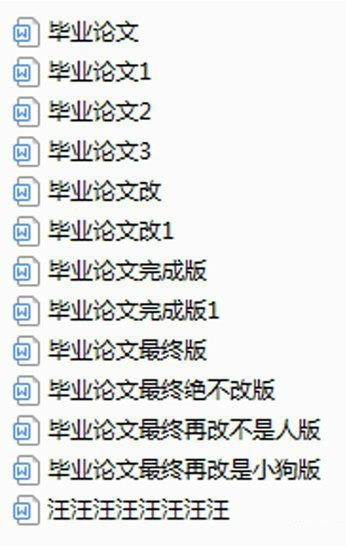
\includegraphics[width=0.95\columnwidth, right]{author-folder/Kai.Wu/thesis_versions.jpg}
    \end{figure}
\end{newminipage}

读到这里,你如果感兴趣可以做个实验,创建一个文件,里面写上一些内容。然后在其他文件夹新建一个同名文件,写上另一些内容。最后,把它拖过来,覆盖掉前面的文件,这时,试一试自己有没有任何办法找回前面文件的内容。

你可能要问,上面不是说了这么多备份方法吗?是的,这些备份方法主要的作用是防丢失,比如电脑丢失、硬盘损坏,但少有备份能做到防覆盖。比如,实时备份的网盘,你本地把文件错误覆盖了,云端也马上被覆盖了。本地备份硬盘,如果备份频率不高,则还有一线生机,但如果过一段时间再去找,也可能找不到了。

因此,为了你的论文(命根子)安全,完全值得再加一层保险:

\begin{enumerate}
    \item Windows开启系统级的文件历史保护:\url{https://www.asus.com.cn/support/FAQ/1013067/},别忘了一定要把你的论文文件夹添加进去才能生效
    \item mac的TimeMachine(时间机器)备份自带了文件历史功能。参照前面的 \ref{sec.pc_backup} 配置好TM,整个电脑的文件历史就都包括在备份里了。
    \item Linux用户,我相信你们有的是办法。最笨的办法,直接写一个shell脚本,把论文文件夹直接复制到其他目录、用日期命名,最后把这个脚本加到crontab里定期运行即可。
    \item 以上是开启本地文件历史的方法。一些网盘自带文件版本功能,但一般限制版本数量或者日期,或者必须要买会员才能开启文件版本。开启过后,相当于云端也存了一份版本历史,万一本地的你没设置好或者其他什么原因不能用,还能在错误覆盖的时候救你一命。学校的seadrive自带大概两个月的文件版本,免费,非常良心,再次建议大家使用。直接把文件夹拖进去备份,就会自动产生文件版本。参见章节 \ref{sec.net_drive_backup} 。
    \item 会一点Git、GitHub的同学,请直接把整个论文文件夹创建成Git项目,并上传到GitHub做成private repo,每天工作结束后交一个commit来备份版本,同时记录你修改了什么内容。对于论文,Git是最完美的备份方案,可以轻松回滚到老版本同时从不担心覆盖、甚至能轻松知道哪个地方的修改是在什么时候引入的,比以上所有方法都靠谱。Overleaf也有GitHub集成,可以方便的与导师协作。但Git学习成本略高,不过网上有无数详尽的教程,感兴趣、学有余力的同学可自行学习。
\end{enumerate}


\begin{flushright}
(2022年12月02日 by \Wu)

(major update: 2022年12月30日 by \Wu)
\end{flushright}

% \begin{figure}[H]
%     \centering
%     \includegraphics[width=0.5\columnwidth]{author-folder/Kai.Wu/}
% \end{figure}


% \usepackage[export]{adjustbox}

% \item 
% \begin{minipage}{0.3\textwidth}
%     文字
% \end{minipage}
% \begin{minipage}{0.63\textwidth}
%     \begin{figure}[H]
%         \includegraphics[width=0.95\columnwidth, right]{author-folder/Kai.Wu/}
%     \end{figure}
% \end{minipage}

% \input{author-folder/Kai.Wu/.tex}
 \clearpage

\section{Remote Control: How to Access Campus Computers from Off-Campus}

When you are off-campus, you might often miss your campus computer. Whether it's the desktop provided by the school or other computers bought with your advisor's funds, they can all be remotely controlled.

\subsection{Preparation for School-Provided Computers}
(If you are not trying to access a school-provided computer, please skip to the next section)

School-provided computers are quite special, and by default, we cannot install software on them. There are two ways to handle this:
\begin{enumerate}
    \item Email or call IT and directly ask for administrator privileges. Just say you are a PhD student and need to install software on the school-provided computer. After that, you can install the control software.
    \item After the above method, the computer is still managed by the school and there are still some restrictions, but it is generally sufficient for regular use. For those who want complete control over the school computer, you can format the disk and reinstall the system, or partition the disk (keeping the original system) and install a dual system. There are many tutorials on reinstalling Windows, partitioning, and setting up dual systems on Bilibili and Zhihu.
\end{enumerate}

\subsection{Recommended Desktop Control Software}
The following software can be used on any system: Windows, Linux, or Mac.
\begin{itemize}
    \item VNC: Install VNC Server on the controlled end (school computer) \url{https://www.realvnc.com/en/connect/download/vnc/}, and VNC Viewer on the controlling end (your computer) \url{https://www.realvnc.com/en/connect/download/viewer/}. Register an account and log in to use, no need to remember connection codes. Recommended because VNC is a well-tested remote desktop solution that generally works as long as the network is stable.
    \item ToDesk: \url{https://www.todesk.com/} Install the same software on both computers. Recommended because it is a new software and generally smoother than VNC.
    \item Others: AnyDesk, TeamViewer, Sunflower, all can be tried. However, TeamViewer is not highly recommended because it might detect the network environment of the school and force you to purchase a commercial version, which is not an issue with other software.
\end{itemize}

\subsection{Remote SSH}
(If you don't use Linux, you can skip to the next section on pitfalls)

If the controlled end is a Linux system and you mainly use command-line operations, connecting via SSH directly will be much faster than desktop control.

The computer on campus has an internal IP starting with 10. How to SSH from outside? This trick is called "NAT traversal."

First, I recommend this video:

\href{https://www.bilibili.com/video/BV1Qq4y1w7F5}{[Hardcore] Public Network Access? NAT Traversal! Zero Experience Start!}\url{https://www.bilibili.com/video/BV1Qq4y1w7F5}

The solutions available for campus machines in the video are:
\begin{itemize}
    \item At 04:52 in the video, using IPV6 connection. However, note that in my experience, the school's IPV6 is unstable and might stop working after a few days. Even if you can set up DDNS, I personally do not recommend it.
    \item A more reliable solution is introduced at 08:09 in the video: NAT traversal. Free and easy-to-use solutions include: Zerotier (slightly slow as it is overseas), Peanut Shell (an old domestic brand, but registration requires an ID card), NOFRP (new, reliability might be low), or directly search "free NAT traversal" on Bilibili for many new solutions. If you are not familiar with these, there are many tutorials on Bilibili and Zhihu.
    \item (Advanced high-traffic version, but with a higher learning curve) Free solutions have limitations on traffic and bandwidth, which are sufficient for SSH commands. But if you want to use SCP to transfer files or forward VNC via SSH, consider renting a cloud server with your advisor's funds and manually setting up an FRP service (a bit complicated, but very smooth once set up, faster than the previous remote desktop solutions). Alternatively, set up a junk machine as a jump server in your dorm with a public IP and DDNS for unlimited traffic access. These solutions have a higher learning curve, but you can refer to online tutorials and experiment slowly.
\end{itemize}

\subsection{Pitfalls}
Here are some experiences I gained after encountering many pitfalls:
\begin{enumerate}
    \item Redundancy to improve reliability: Do not rely on a single remote control solution. If one fails, you can use another. Please install at least two, and if you are away for a long time, install more. I personally use: a second-hand thin client at home with FRP and DDNS + Peanut Shell as a backup plan + VNC as another backup plan + ToDesk, a four-layer backup solution for stable access to my campus Linux computer.
    \item After installation, restart once to see if the control software can start automatically.
    \item If the controlled end is a Windows computer, be sure to disable system updates. Although restarting is fine, a major Windows update might get stuck on a screen asking you to agree to a new user agreement, and unless you are there to click it, no software will start, and you will lose control. Please search "disable Windows updates" on Baidu. I personally recommend using a combination of group policy and host file modification.
    \item For those running programs, be sure not to exceed memory limits or crash the system memory. If the memory is fully used, the system will crash immediately, killing all control software, and it will not restart automatically. You must be there to force a restart. Please find ways to monitor and control memory usage in your programs.
    \item If possible, purchase remote KVM hardware like "Sunflower Control" to force a remote restart even if the system crashes.
    \item No matter how good the solution is, it cannot prevent network maintenance or power outages on campus. These can be defended against. For network outages, make sure to check the macauth option when logging in to the network, so it will work again after maintenance. For power outages, the motherboard needs to support the "boot on power" or "boot with power" function. Check the motherboard manual or search for "power" to see if it is available. Alternatively, purchase Sunflower Control. However, power and network outages are rare, and unless you are away for months, you generally do not need to worry about them.
    \item Maintain a good relationship with at least one on-campus classmate. Newcomers will encounter various unexpected situations and lose control, requiring office classmates to help check the machine. Behind 100 remote control solutions, you also need good classmates for physical control. In case the network cable is accidentally kicked out, you still need a classmate to help you fix it.
\end{enumerate}

\begin{flushright}
(09 November 2022 by \Wu) \\
Translated by GPT
\end{flushright}
 \clearpage

\section{我的老腰受不了了——如何保持颈椎、腰椎健康}

\subsection{缓解腰的问题:升降桌}

\begin{newminipage}[0.39]
    \begin{figure}[H]
        \includegraphics[width=0.95\columnwidth, right]{author-folder/Yue.Zhou/gongzuotai.jpg}
    \end{figure}
\end{newminipage}
\begin{newminipage}[0.6]
    在没有读博之前,我就患上了严重的腰肌劳损。这个玩意怎么说呢,说是大病吧,他不是,但无时无刻不在折磨着你。最严重的时候,疼的我晚上都睡不着。去医院看过也开过药,但医生说这个病需要自己保养,无法根治。后来我试着跑了半年步,哎!腰肌劳损神奇的好了,现在一点都不疼了(如遇久坐,仍旧是不行的,会疼)。读博之后也没有心情运动了,于是买了一个升降工作台(推荐人手一个!太好用了!)。可以站着办公,站累了就坐下办公。极大程度上杜绝了久坐对腰椎的伤害。
\end{newminipage}

\begin{flushright}
(2022年12月30日 by Yue Zhou)
\end{flushright}

\subsection{来自重度腰椎间盘突出、颈椎病患者的深度建议}

\subsubsection{升降桌:可极大缓解腰椎问题,但不能完全解决}

我十年腰椎间盘突出加五年颈椎病,19年的时候腰就疼到没法坐一整天,就在实验室放了台升降桌,站着用了三年电脑。今年还在卧室里放了同款升降桌。但长期站着和坐着一样对腰不好,最后会变成站着和坐着一样会腰疼。升降桌不是长久之计,站着只是换了角度继续损耗腰椎。

不能完全依赖升降桌:这几年太依赖升降桌,导致现在长时间站着和坐着一样腰疼,去拍核磁医生都问我是不是腰骨折了。如果真的想缓解腰疼,就要避免久坐久站。中学教师容易得腰疼一方面就是因为站着讲课时间长了。

总之升降桌可以用,但不能长期用它代替坐着用电脑。可以交替用,平时再多锻炼就行。

注意事项:升降桌记得没事调一调高度。我放实验室里的升降桌几年没调好像液压杆生锈了,都调不动了,直接变成了一般桌子。

\subsubsection{外接屏:避免和缓解颈椎病}

颈椎病难受的一点就是,低头时间长就脖子疼,出门在地铁高铁上我都不得不把手机竖起来抬高和眼平行,不然用不了太长时间。

我再贡献一个避免和缓解颈椎病的方法,就是不要长时间用笔记本电脑,长时间低头看屏幕会演变成颈椎病。低头看手机也是。

如果常用笔记本电脑就要在卧室和办公室都放一个台式机屏幕当外接屏。

我颈椎病就是高强度用了一年笔记本电脑得上的,后来只用外接屏就不再继续加重了。

如果经常高强度用笔记本电脑,不用外接屏的话和整天低头用手机一样都是颈椎杀手。我在实验室看见有人长时间用笔记本都会劝他们用外接屏。

笔记本支架也可以,比显示器便宜。但如果视力不好,还是尽量外接屏,因为笔记本屏幕太小了,费眼。我以前也买了很多笔记本支架,现在都用来放显示器了,笔记本刚好能放在下面很方便。

\begin{figure}[H]
    \caption{我自己在卧室里就是升降桌,配笔记本支架。这个组合很适合我这种主要用笔记本的}
    \includegraphics[width=0.95\columnwidth, center]{author-folder/Jialin.Wang/shengjiangzhuo.jpeg}
\end{figure}


% \subsubsection{进一步缓解:趴着用电脑}

% 我今年起站也不能站太长时间,已经开始探索平躺和俯卧用电脑了。平躺我试过几天就放弃了,容易睡着。我觉得平躺就适合看看电影玩游戏。

% 俯卧我最近试了一个月,感觉还行,起码支起上半身不会犯困。

% 我是放了一个便携屏幕在床边,然后配一个趴枕,这样能趴一整天。趴枕好处是吃完饭趴着不会压迫腹部导致不适。

% \begin{figure}[H]
%     % \centering
%     \includegraphics[width=0.3\columnwidth, center]{author-folder/Jialin.Wang/pazhen.jpeg}
% \end{figure}

% 然后配一个可以调角度的笔记本支架放屏幕键盘和鼠标——其实直接放笔记本也行,但发热量大,搬来搬去不方便。用便携屏能快速在升降桌和俯卧之间切换——我也想过买一般的显示器支架,但没有卖那种适合在床上用的,而且一般显示器在床上用太大了。便携屏就是笔记本二手屏幕改装的,大小和笔记本电脑一样在床上用正好。

% 如果长时间趴着用电脑,我发现最好是用双臂稍微用力撑起上半身。但上半身主要还是靠着躯干受力,双臂是辅助作用,避免下巴受力太大。

% 我现在已经练成了能俯卧一天的神功,笔记本支架只要调好角度,让手和手臂平行,这样手腕就不会因为长时间弯曲而酸痛。

% 不过最近因为趴习惯了加上天冷就完全不锻炼,如果不趴着,还是腰疼。还是得坚持锻炼才行。

% 这一套方案我觉得真的完美适合我这种腰疼到无法长时间坐着和站着的人,但这些都不能治好腰疼。锻炼才是最重要的。时间长不锻炼,不常用的肌肉会萎缩,更不好。(我好想以后住在热带沿海地区,每天傍晚去海边游泳,傍晚的时候海水是温的)


\subsubsection{最好的解决方案:改变生活习惯、加强锻炼}

建议有腰椎间盘突出和颈椎病的人还是多锻炼。但不要盲目去健身房锻炼,最好的锻炼方法还是游泳,因为其他锻炼方式大多会需要腰部用力,加重腰疼。

我目前只是偶尔腰疼到不能弯腰。我还认识腰疼到走路一瘸一拐的,他也是慢慢锻炼才逐渐好转。

如果自制力不强,加学校游泳社团也行,起码有人经常一起去锻炼能有动力。

办卡的话,我记得每年九月份独墅湖游泳馆能办半价年卡,但学校社团很便宜,更划算。以前我办游泳卡前每周都跟着学校游泳社团去游一两次,办了年卡后,一年去了不到五次,后来就去得更少了。
如果自制力可以,每天锻炼是最好的方法。
如果坚持不下去,还无法改变生活习惯,就会越来越严重。

最后,如果腰疼比较严重,有空可以去医院骨科看看,做一下核磁,看一下腰椎到底发展到哪个地步,来决定怎么具体该恢复。现在腰疼在年轻人里很普及。

\begin{flushright}
(2022年12月30日 by Jialin Wang)
\end{flushright} \clearpage

\section{Liverpool Visit}
\label{section.UoL_visit}

\subsection{Potential Opportunities}
\subsubsection{Collaboration with Liverpool Supervisors}
Although most students will have a supervisor from Liverpool on their team, each project may be different, and you may not have frequent interactions with them before going to Liverpool. This infrequency could be due to various reasons, not necessarily because your work is in a different field. So if you think it would be interesting to collaborate with them in Liverpool, please prepare in advance.

If you haven't had much interaction with them before, make sure to establish some familiarity through some means, which will make future collaboration smoother. This can be through video meetings or emails sharing your research progress and plans, co-authoring papers, or brainstorming potential collaborative research content in advance.

We know that teamwork can happen for different reasons (see \ref{subsection.teamwork}), but in any case, be sure to confirm at least the general direction of your activities during your visit with your Liverpool supervisor in advance, including but not limited to: things that require their involvement, schedule, things you need to prepare, and things you plan to do.

\subsection{Accommodation and Living}
\href{https://hallslife.liverpool.ac.uk}{Halls Life} is the community hub for student accommodation at the University of Liverpool, providing various suggestions on accommodation and living. It is strongly recommended to browse it before departing for the UK, as it can help decide whether to bring certain luggage.

\subsubsection{Visiting Other University Libraries}
When you are traveling and visiting various universities in the UK, if you happen to pass by a university library when you are tired, you can actually go in and sit down, as long as you have applied for \href{https://access.sconul.ac.uk/sconul-access}{SCONUL Access} in advance.

Although different libraries have different policies, in most cases, you can at least enter the library after successfully applying, and some libraries may also provide computer access or book borrowing privileges.

\begin{quote}
    Q. Do I need to complete an online application for each institution I would like to visit?
    
    A. No, although you do need to indicate a library you are interested in visiting as part of your application, your approval email allows you to visit any of those libraries on the list. You do not need to reapply. \hfill 21 Oct, 2024 from \href{https://access.sconul.ac.uk/page/access-faq#Multiple%20applications}{Access FAQ | SCONUL}
\end{quote}

After submitting the application, it will be processed by the University of Liverpool Library, and once approved, you can go to the front desk of each university library with the email to get a visitor card.

\subsection{Food and Entertainment}
\href{https://hallslife.liverpool.ac.uk}{Halls Life} is the community hub for student accommodation at the University of Liverpool, providing various suggestions on food and entertainment.

\begin{flushright}
    October 21, 2022 by \Shiyao

    Translated by GPT
\end{flushright}
 \clearpage

\section{XJTLU Virtual Machine}
\url{https://vdi.xjtlu.edu.cn/portal/webclient/index.html}
If you are outside the university and want to quickly access on-campus resources and software temporarily, you can use the university's online virtual machine. The virtual machine is equivalent to a computer located on campus.

\section{Library Literature Databases}
After connecting to the campus network, most of the journals subscribed by the university can be directly downloaded from the journal pages. However, (1) some journal websites cannot recognize your IP, such as the famous Annual Review series; (2) if you want to download papers off-campus, you can use the library's literature databases.

\begin{figure}[H]
    \includegraphics[width=0.7\columnwidth, center]{author-folder/Kai.Wu/library-ejournal.jpg}
\end{figure}

What I use most is clicking e-journal on the homepage \url{https://lib.xjtlu.edu.cn}, searching for the journal by name, and then accessing it through a dedicated link. The library also provides many full-text databases, including CNKI and other Chinese journal databases. For detailed usage, see the library's past training sessions \url{https://core.xjtlu.edu.cn/course/view.php?id=905}, or directly find the PPT in this project's GitHub (\href{https://github.com/xp-pgrs-unofficial-guide/xp_pgrs_unofficial_guide/tree/main/fileshare}{link}).

\section{Borrowing Books from Suzhou Library and Free Book Delivery}
If you want to read books from Dushu Lake Library or borrow books from Suzhou Library but don't want to go there because it's too far, what should you do? Just use the mini program to borrow books! Books from Suzhou Library can be \textbf{[free of charge]} delivered to Dushu Lake Library for pickup, and books from Dushu Lake Library can be directly delivered to the entrance of the university library.

Search for the mini program "Suzhou Library Borrow Books" on WeChat. Since the medical insurance card is the citizen card, you can use it to borrow books directly. If you have already obtained the medical insurance card, you can bind it directly to waive the card opening fee. Then follow the prompts in the mini program.

% \section{Student Medical Insurance}
\section{Pay Attention to Your Negative Emotions and Depression Tendencies}
\label{sec.mental_health}

\begin{figure}[H]
    \includegraphics[width=0.6\columnwidth, center]{author-folder/Kai.Wu/mental_1.pdf}
    \includegraphics[width=0.6\columnwidth, center]{author-folder/Kai.Wu/mental_2.pdf}
    \includegraphics[width=0.6\columnwidth, center]{author-folder/Kai.Wu/mental_3.pdf}
\end{figure}

The \href{http://ga.berkeley.edu/wellbeingreport}{Graduate Student Happiness and Well-Being Report [link]} published by the Berkeley Graduate Assembly in 2014 shows that 46\% of Ph.D. students have mental health problems. Studies published in authoritative journals such as Nature suggest:
\begin{enumerate}
    \item Graduate students are six times more likely to suffer from severe anxiety and depression than the general population \href{https://www.nature.com/articles/nbt.4089}{[reference link]}
    \item Smarter people are more likely to suffer from mood disorders such as anxiety or depression but are less likely to seek help \href{https://www.nature.com/articles/nj7677-549a}{[reference link]}
    \item Mood disorders account for 80-90\% of suicides \href{https://www.sciencedirect.com/science/article/pii/S0160289616303324}{[reference link]}
    \item During the COVID-19 pandemic, four out of five researchers showed signs of mental health distress \href{https://www.tandfonline.com/doi/full/10.1080/21568235.2021.1992293}{[reference link]}
\end{enumerate}

\begin{figure}[H]
    \begin{tabular}{rcl}
        \includegraphics[width=0.31\columnwidth]{author-folder/Kai.Wu/chat1of3.jpg} &
        \includegraphics[width=0.31\columnwidth]{author-folder/Kai.Wu/chat2of3.jpg} &
        \includegraphics[width=0.31\columnwidth]{author-folder/Kai.Wu/chat3of3.jpg}
    \end{tabular}
    \caption{Chat records with a graduated classmate. The incidence of depression among our university's Ph.D. students is higher than imagined}
\end{figure}

As a high-risk group, we have received extensive professional knowledge and skills training, yet almost no one has taught us "how to maintain mental health." If you often feel nervous, anxious, or disappointed now, and even have symptoms like insomnia, please immediately face your situation, put your health first, and feel free to seek help from the university's psychological counseling center.

Meanwhile, prevention is always more effective than post-treatment. I hope that everyone reading this, whether you feel good now or not, will click the links below, read Zoe Ayres' lecture in Liverpool (the source of the above PPTs), and her book "\textit{Managing Your Mental Health During Your PhD - A Survival Guide}," to get through your graduate studies healthily. ~~\href{https://github.com/xp-pgrs-unofficial-guide/xp_pgrs_unofficial_guide/tree/main/fileshare}{[GitHub link]}~~~~~\href{https://gitee.com/kaiwu-astro/xp_pgrs_unofficial_guide/tree/main/fileshare}{[Use this link if you can't access GitHub]}

\section{What Software Have You Installed on Your Computer? (Looking Forward to Your Additions)}

\KW: Let me start by sharing some software that I would definitely recommend to my fellow junior students:
\begin{figure}[H]
    \includegraphics[width=\columnwidth]{author-folder/Kai.Wu/kai_mac_dock.jpg}
\end{figure}
\begin{itemize}
    \item Research and Productivity Tools
    \begin{enumerate}
        \item Notion (All platforms). An incredibly powerful new-generation note-taking app. I was originally a heavy OneNote user, but after being introduced to Notion by chance, I decided to abandon OneNote and completely switch to Notion after a short trial. Recommended because: supports Win/Mac/Linux/Web/iOS/Android; powerful database functions to perfectly build your own GTD system and greatly improve efficiency; fast global search; modern collaboration features, even usable for team and project management; powerful sharing features to easily share notes as public webpages; lots of tutorials on Bilibili.

        \includegraphics[width=0.8\columnwidth]{author-folder/Kai.Wu/notion.jpg}
        \item TickTick (All platforms). I've used Wunderlist (later acquired by Microsoft and became Microsoft To-Do), iOS's built-in Reminders, and several other list apps for a long time. Only TickTick feels the most intuitive and user-friendly. Used together with Notion, it can conveniently manage all aspects of study and life. Supports all platforms.

        \includegraphics[width=0.8\columnwidth]{author-folder/Kai.Wu/dida.jpg}
        \item Trello (All platforms). Manage your to-do items and tasks with cards. My supervisor heavily relies on Trello to keep his numerous tasks well-organized. While I think Notion is a superset of Trello, if you don't like Notion for some reason, at least try Trello. Available for download on all platforms.

        \includegraphics[width=0.8\columnwidth]{author-folder/Kai.Wu/trello.jpg}
        \item VSCode (Visual Studio Code) (All PC platforms). An open-source text editor that rose to prominence around 2019, with extremely strong community and plugin support. Currently, I use VSCode + LaTeX Workshop plugin for my journal papers, theses, and even this guide you're reading. All my numerical simulation programs and data analysis scripts are also done with VSCode. The drawbacks are a small learning curve and the need to configure settings; it also consumes memory like Chrome.

        \includegraphics[width=0.8\columnwidth]{author-folder/Kai.Wu/vscode.jpg}
        \item Spark. An email app developed by Readdle, an award-winning Apple app developer, that manages all your email accounts in one place and syncs email settings to the cloud, solving the problem of re-adding multiple email accounts when you get a new device. It seems to be exclusive to Mac and iOS; not sure if it's available on other platforms.

        \includegraphics[width=0.8\columnwidth]{author-folder/Kai.Wu/spark.jpg}
        \item As for reference management software, I won't make recommendations—everyone has their own preferences. If you don't have one yet, ask your seniors or check out recommendations on Bilibili.
    \end{enumerate}
    \item Efficiency Tools
    \begin{enumerate}
        \item Bob (MacOS) or Pot (Win/Mac/Linux). Tools for word translation, screenshot translation, and OCR. Supports integration with ChatGPT, DeepL, Google Translate, Youdao Translate, and other translation services, and can even display results from multiple platforms simultaneously for comparison. Bob can be downloaded from the Mac App Store; Pot is available at pot-app.com.

        \includegraphics[width=0.8\columnwidth]{author-folder/Kai.Wu/Bob.jpg}
    \end{enumerate}
\end{itemize}

Have you discovered any great software? Please feel free to share them with your fellow junior students.

Your recommendations:

\begin{flushright}
    Translated by GPT
\end{flushright}
% \chapter{避坑指南(待补)}


\section{一个坑}
如果你踩过什么坑,可以花两分钟告诉我,标记在这里,免得大家一起踩坑,\sout{形成喜闻乐见的场面}
% % \chapter{非西浦本科生必看的额外攻略(挖坑待补)}
\label{chapter.non-xjtluer}

\section{食堂办卡可打9折}
% % \chapter{PGR Society 社团(社长你来写这部分)}

介绍
% \chapter{写作指南}
\label{chapter.author-ins}

% v0.1 by Kai.Wu

你用十几分钟写下的经验,可能会节约下后来人几小时甚至几天的时间。欢迎为本攻略做出贡献。

最简单粗暴的贡献方式,直接把纯文本、word或者tex文件发给 \Shiyao。管理员会帮你把文件转换成\LaTeX{}格式放进攻略。虽然管理员可能没有那么开心,因为要费些时间建文件整理上传,但也是可以的。如果你心疼可怜的管理员,可以看看下面的方法(嫌麻烦的同学可以跳过下面的部分,直接看本页最后一段话)。更好的投稿姿势:


\begin{itemize}
    \item 如果你有使用Git和交Pull Request的经验,也会写\LaTeX{},那么可以直接在\href{https://github.com/xp-pgrs-unofficial-guide/xp_pgrs_unofficial_guide}{本手册的GitHub页面}提交PR。\href{https://www.zhihu.com/question/21682976/answer/79489643}{如何交PR可参照这个链接}
    % \item 如果你不会交PR,但会写\LaTeX{},可以在Overleaf上写。请发邮件到 Kai.Wu19 at student.xjtlu.edu.cn 申请编辑权限。写完过后,请发邮件给管理员把稿件推送到GitHub。
\end{itemize} 

\vspace{5mm}
注意:对于上面高级的投稿方法,为避免多人协作弄乱顺序,请每位作者在\texttt{author-folder}文件夹下建立自己的子目录,在里面新建\texttt{tex}文件写作,第一行直接从\texttt{section}命令开始,其后写正文。写完了过后,在正确的章节里,用以下代码把你的稿件插入到\texttt{chapter}文件夹下的章节里
\begin{lstlisting}
    \input{你的tex文件路径}
\end{lstlisting} 
例如,王多鱼同学想要分享自己的常用软件。首先在\texttt{author-folder}下建立一个\texttt{duoyu.wang}文件夹,在里面新建\texttt{health-insurance-use.tex},第一行写\lstinline[breaklines=true]!\section{学生医保使用}!写标题,后面写正文。写好过后,在\texttt{chapters}文件夹里的\texttt{others.tex}中,添加一行\lstinline[breaklines=true]!\input{author-folder/duoyu.wang/health-insurance-use.tex}!,就完成了。

\vspace{5mm}
如果要一些高级的编辑方式,可参照项目 GitHub 的\texttt{author-guide}目录下的模板手册和例子。

\vspace{5mm}
属不署名都可以。可以匿名,也可以把姓名邮箱院系入学年份都写上。你如果愿意的话把生辰八字、出生年月、房产车产详情附上也是完全可以的,这样甚至可以问问PGR Society能不能安排相亲(雾)。最后必须要提醒:您不得发布任何违反中华人民共和国法律、西交利物浦大学博士生守则、\href{https://www.liverpool.ac.uk/aqsd/academic-codes-of-practice/pgr-code-of-practice/}{利物浦大学博士生守则}和其他任何适用规定的内容。您需要对你发布的内容负责,PGR Society无法对内容的准确性做担保或审核。由您发布的内容导致的任何纠纷,PGR Society社团和其他作者不承担任何连带责任。

\vspace{5mm}
再次感谢你为学弟学妹们、祖国的花朵们做出的贡献  (ง •̀\_•́)ง
% \chapter{附录}
\label{sec.appendix}

\section{校园地图}
\begin{figure}[H]
    \includegraphics[width=\columnwidth]{author-folder/Kai.Wu/XJTLU-campus-map.pdf}
\end{figure}

\clearpage
% \section{校历:哪天放假}
% 独立的校历文件可在本项目的GitHub里(\href{https://github.com/kaiwu-astro/xp_pgrs_unofficial_guide/raw/main/author-folder/Kai.Wu/Academic_Calendar-202223.pdf}{链接})找到。
% \begin{figure}[H]
%     \includegraphics[width=0.9\columnwidth]{author-folder/Kai.Wu/Academic_Calendar-202223.pdf}
% \end{figure}

\section{学校电话}

\begin{table}[H]
    \begin{tabular}{p{60mm}cc}
        \hline
        部门 & 电话 & 邮箱 \\ \hline
        Academic Services Office \newline 学术服务 & 8188 4754 & aso@xjtlu.edu.cn \\ \hline
        Alumni Service \newline 校友服务           & 8816 1869 & alumni@xjtlu.edu.cn \\ \hline
        Campus Management Office\newline 校园管理办公室 & 8816 1071 & cmo@xjtlu.edu.cn \\ \hline
        Career Service \newline 就业服务           & 8188 8308 & careers@xjtlu.edu.cn \\ \hline
        IT Service Centre \newline IT服务中心      & 8816 1250 & it@xjtlu.edu.cn \\ \hline
        Library \newline 图书馆                    & 8816 1290 & askalibrarian@xjtlu.edu.cn \\ \hline
        Media Service \newline 新闻线索与媒体服务    & 8816 1351/1032 & news@xjtlu.edu.cn \\ \hline
        Postgraduate Recruitment \newline 研究生招生 & 8816 1889/7111 & pgenquiries@xjtlu.edu.cn \\ \hline
        President's Office \newline 校长办公室     & 8816 1004 & president.office@xjtlu.edu.cn \\ \hline
        Registry \newline 教务办公室               & 8816 1230 & registry@xjtlu.edu.cn \\ \hline
        Research Management Office \newline 科研管理办公室 & 8816 1139 &  \\ \hline
        Student Onestop Centre \newline 学生一站式 & 8816 1854 & onestop@xjtlu.edu.cn \\ \hline
        XJTLU Global (Support) \newline 西浦国际 & 8897 3094/3093 & global@xjtlu.edu.cn \\ \hline
    \end{tabular}
\end{table}


%======================================================================
\backmatter	
% \chapter{Acknowledgements}
\begin{itemize}
    \item This manual uses the ElegantBook template \url{https://github.com/ElegantLaTeX/ElegantBook}
    \item \Wu \space would like to thank MB321's Chengyu Wang, Francesco Flammini Dotti, Xiuming Xu, Yu Wang (in alphabetical order) and other seniors for their great help during the first two years of PhD, especially in the introduction of gym facilities, obtaining office supplies, supervisory meeting records, and APR. Thanks to classmates from 22-AoFE-Tian, 2023-InD-Rolf for corrections, and 22-ARC-Yang for information supplements. Thanks to other authors for their hard work.
    \item \Shiyao \space would like to thank \Wu \space for founding this project in August 2022 and editing a large amount of content in this manual over two years.
    \item (Other authors, please add your acknowledgements here)
\end{itemize}


% In the future, we might even get some sponsors to fund activities, organize outings for PhD students, etc.

\begin{flushright}
    Translated by GPT
\end{flushright}
% \chapter{更新日志}

本页面由项目管理员维护,只记录大版本更新。小版本更新内容,可到 \href{https://github.com/xp-pgrs-unofficial-guide/xp_pgrs_unofficial_guide/commits/main}{GitHub commit 页}查询。

\begin{itemize}
    \item v0.1 on 2022/8/9:完成项目创建,确定模板,构建GitHub Actions自动在线编译并发布
    \item v0.2 on 2022/10/12:完成[必做]、[福利]两大章节的攻略内容,包括必修课程、会议记录、APR、会议经费、办公用品、打印、体育馆
    \item v0.3 on 2022/11/18:完成[最好要知道]章节的绝大部分内容:TA的改作业、监考、lab,Symposium(移动到[必做]章)
    \item v0.4 on 2023/03/01:新增电脑备份攻略、腰椎颈椎攻略、学生证相关攻略、常用信息导航
    \item v1.0 on 2024/08/12:补完毕业章节
    \item v1.1 on 2024/10/21:新增 \ref{section.how-research-works} 节 \space 学术研究是怎么发生的、 \ref{section.UoL_visit} 节 \space 利物浦访学
\end{itemize}





\makeatletter
\makeatother
\end{document}
